%!TEX TS-program = xelatex
%!TEX encoding = UTF-8 Unicode
%!TEX root = .

\documentclass{Dissertate}
\usepackage[a-3b]{pdfx}
\usepackage[english]{babel}
\usepackage{titlesec}
\usepackage{fontspec}
\usepackage{amsbsy}
\usepackage{stmaryrd}
\usepackage{enumitem}
\usepackage{proof}
\usepackage[export]{adjustbox}
\usepackage{amsmath,amssymb,amsfonts,amsthm}

% Coding
\usepackage{listings}
\usepackage{xcolor}
\usepackage{comment}

\newtheorem{theorem}{Theorem}[section]
\providecommand*\theoremautorefname{Theorem}

\newtheorem{lemma}{Lemma}[section]
\providecommand*\lemmaautorefname{Lemma}

\newtheorem{definition}{Definition}[section]
\providecommand*\definitionautorefname{Definition}

\newtheorem{corollary}{Corollary}[section]
\providecommand*\corollaryautorefname{Corollary}

\newtheorem{proposition}{Proposition}[section]
\providecommand*\propositionautorefname{Proposition}

\newtheorem{exercise}{Exercise}[section]
\providecommand*\excerciseautorefname{Exercise}

\newtheorem{example}{Example}[section]
\providecommand*\exampleautorefname{Example}

\providecommand*\algorithmautorefname{Algorithm}

\newenvironment{solution}{\noindent Solution.}{\hfill$\Box$}

\newcommand{\ltl}{LTL}
\newcommand{\pastltl}{LTL+P}
\newcommand{\ebrltl}{\ltl_{EBR}}
\newcommand{\pastebrltl}{\ltl_{EBR}+P}
\newcommand{\fpltl}{\ltl_{FP}}
\newcommand{\fbltl}{\ltl_{FB}}

\newcommand{\ltlTrue}{\top}
\newcommand{\ltlFalse}{\bot}
\newcommand{\ltlNeg}[1]{\neg #1}
\newcommand{\ltlAnd}[2]{#1 \land #2}
\newcommand{\ltlOr}[2]{#1 \lor #2}
\newcommand{\ltlImpl}[2]{#1 \to #2}
\newcommand{\ltlIff}[2]{#1 \iff #2}
\newcommand{\ltlX}[1]{\mathbf{X} #1}
\newcommand{\ltlZ}[1]{\mathbf{Z} #1}
\newcommand{\ltlXexp}[2]{\mathbf{X}^{#2} #1}
\newcommand{\ltlY}[1]{\mathbf{Y} #1}
\newcommand{\ltlG}[1]{\mathbf{G} #1}
\newcommand{\ltlGbounded}[2]{\mathbf{G}^{#2} #1}
\newcommand{\ltlF}[1]{\mathbf{F} #1}
\newcommand{\ltlFbounded}[2]{\mathbf{F}^{#2} #1}
\newcommand{\ltlO}[1]{\mathbf{O} #1}
\newcommand{\ltlH}[1]{\mathbf{H} #1}
\newcommand{\ltlU}[2]{#1 \mathbf{U} #2}
\newcommand{\ltlS}[2]{#1 \mathbf{S} #2}
\newcommand{\ltlT}[2]{#1 \mathbf{T} #2}
\newcommand{\ltlR}[2]{#1 \mathbf{R} #2}
\newcommand{\ltlUbounded}[3]{#1 \mathbf{U}^{#3} #2}

\newcommand{\ltlB}[3]{B_{#2}^{#3}{#1}}

\newcommand{\sequence}[1]{\left\langle #1 \right\rangle}
\newcommand{\lang}[1]{\mathcal{L}{#1}}
\newcommand{\omegalang}[1]{\lang{}_\omega{#1}}
\newcommand{\logic}{\mathbb{L}}
\newcommand{\automaton}{\mathcal{A}}
\newcommand{\semantics}[1]{\llbracket #1 \rrbracket}
\newcommand{\model}{\mathcal{M}}

\newcommand{\arena}{A}
\newcommand{\game}{G}
\newcommand{\C}{C}
\newcommand{\U}{U}

\newcommand{\closedloop}[2]{#1 \times #2}
\newcommand{\controller}{C}
\newcommand{\plant}{P}
\newcommand{\eval}[2]{eval_{#1}{#2}}

\newcommand{\modelsBV}[1]{\models_{#1}}
\newcommand{\modelsBE}[1]{\models_{#1}^{BE}}

\newcommand{\modelsUB}[2]{\models_{#1}^{#2}}
\newcommand{\modelsASAP}[2]{\models_{{#1}^*}^{#2}}

\newcommand{\TD}{TD}
\newcommand{\D}{D}

\definecolor{codegreen}{rgb}{0,0.6,0}
\definecolor{codegray}{rgb}{0.5,0.5,0.5}
\definecolor{codepurple}{rgb}{0.58,0,0.82}
\definecolor{backcolour}{rgb}{0.95,0.95,0.92}

\lstdefinestyle{mystyle}{
    backgroundcolor=\color{backcolour},   
    commentstyle=\color{codegreen},
    keywordstyle=\color{magenta},
    numberstyle=\tiny\color{codegray},
    stringstyle=\color{codepurple},
    basicstyle=\ttfamily\footnotesize,
    breakatwhitespace=false,         
    breaklines=true,                 
    captionpos=b,                    
    keepspaces=true,                 
    numbers=left,                    
    numbersep=5pt,                  
    showspaces=false,                
    showstringspaces=false,
    showtabs=false,                  
    tabsize=2
}

\lstdefinelanguage{smv}{
    morekeywords={
        MODULE, VAR, IVAR, INVARSPEC, DEFINE, ASSIGN, FROZENVAR,
        PARSYNTH,
        integer, boolean,
        TRUE, FALSE,
        init, next, case, esac,
        LTLSPEC,INVARSPEC,CTLSPEC
    },
    sensitive=false, % keywords are not case-sensitive
    morecomment=[l]{--}, % l is for line comment
    morestring=[b]" % defines that strings are enclosed in double quotes
} %

\lstset{style=mystyle}


\newcommand{\enumpar}{(\arabic*)}
\newcommand{\Nat}{\mathbb{N}}
\newcommand{\Int}{\mathbb{Z}}
\newcommand{\Real}{\mathbb{R}}
\newcommand{\Bool}{\mathbb{B}}
\newcommand{\domain}{\mathbb{D}}
\newcommand{\card}[1]{\left\lvert #1 \right\rvert}
\newcommand{\set}[1]{\{ #1 \}}
\newcommand{\tuple}[1]{\left( #1 \right)}
\newcommand{\eqdef}{\ensuremath{\stackrel{\triangle}{=}}}


\begin{document}

% the front matter
%!TEX root = ../main.tex
\title{Model checking and synthesis of best-effort strategies for safety and co-safety LTL}
\author{Filippo Fantinato}

% If you have one advisor
\advisor{Professor Davide Bresolin}

% If you are coadvised
\coadvisorOne{Doctor Stefano Tonetta}
\coadvisorOneUniversity{Fondazione Bruno Kessler}

\university{University of Padova}
\department{Mathematics “Tullio Levi-Civita”}
\mastername{Computer Science}
\academicYear{2022-2023}

\frontmatter
\setstretch{\dnormalspacing}

% include each chapter...
\setcounter{chapter}{0}  % start chapter numbering at 1
%!TEX root = ../main.tex

\chapter{Introduction} \label{chapt:introduction}

In Computer Science there has always been the need to prove the correctness of systems, in order to have mathematical proofs which state that some properties hold on them. 
The field that deals with proving the correctness of systems is called Formal Methods. 
There are many techniques that fall within the Formal Methods field, but the most popular are those techniques which generate automated proof of correctness. 
Some of them are: Automated Theorem Proving, in which a system attempts to produce a formal proof from a description of the system, a set of logical axioms, and a set of inference rules; Abstract Interpretation, in which a system verifies an over-approximation of a behavioural property of the program, using a fixpoint computation over a (possibly complete) lattice representing it; Model Checking, in which a system verifies certain properties by means of an exhaustive search of all possible states that a system could enter during its execution.

An interesting and widely used technique which belongs to the Model Checking field is Automaton-based LTL Model Checking.
Such technique exploits a model of the system described as a reactive system via either a Labeled Transition System (LTS), a Moore Machine or a Mealy machine, to prove linear-time properties on it.
Linear-time properties are properties which describe a behaviour along time, assuming that the time is linear (at any time there exists exactly one previous moment and exactly one subsequent moment in time, excepting at the starting time).
To describe linear-time properties we use a logic named Linear Temporal Logic ($\ltl$).
We can group in classes all linear-time properties, to form a hierarchy class of properties with increasing complexity.
The two classes we are interested in are called safety and co-safety.
The first type of class express the concept that "something bad will never happen", while the latter one express the concept that "something good will eventually happen".

Another field which is related to Automaton-based LTL Model Checking is Reactive Synthesis. 
In this field we do not mind anymore to verify a property on a model, but we want to generate automatically a correct-by-construction system starting from some $\ltl$ specifications.
Therefore, we state the $\ltl$ specifications which must hold and we generate a system on which they will hold.
All approaches to solve Reactive Synthesis problems are based on game theory, in particular we can look at such problem like a two-players infinite-game on finite graphs, also called arenas. 
Such problem can be reduced to find out a winning strategy for a given player according to a winning condition. If such winning strategy does not exist, then we say that such game is unrealizable.
There are several types of games, each of which allows to synthesize a particular class of $\ltl$ formulas.  
Full $\ltl$ synthesis is a very complex problem and also expensive in terms of space and time, but we could limit ourselves to synthesize only some $\ltl$ fragments. 
We choose safety and co-safety fragments and the corresponding game are called safety and reachability games, respectively.

This thesis is about the work carried out at Fondazione Bruno Kessler (FBK) with the Formal Methods for System and Software Design unit.
All topics touched upon during the thesis are part of Model Checking and Reactive Synthesis fields. They go from the basics, such as B\"uchi Automata and $\omega$-regular languages, Linear Temporal Logic (LTL) and Automaton-based Model Checking, to more advanced topics, like Reactive Synthesis of safety and co-safety properties from a LTL dialect called $\pastebrltl$, which has the same expressiveness of the safety fragment of $\ltl$.

The problem we have introduced and we have faced is an optimality test on closed-loop models of a system.
Closed-loop models of a system are a very common way to describe abstraction of systems, since they allow you to split the behavioural logic (controller) from the actual system (plant). The controller is another model which reads in input the current state of the plant and reacts consequently to change the state of the plant.
In particular, given a plant, a controller and a safety or co-safety $\ltl$ formula, we want to figure out whether the formula is satisfied in the closed-loop between plant and controller and whether the controller is the best one for that plant according to an optimality principle.
In other words, we want to find out another controller which does better than the current one.
If we cannot find it, then the current controller is optimal.

We introduce formally the problem, presenting two new semantics called bounded-value and best-effort semantics useful to describe it.
Furthermore, we introduce two further semantics, called bounded-steps and As Soon As Possible (ASAP) semantics, which capture the property of a system to act in as little as number of steps.
Later we prove that the ASAP semantics can be expressed in the best-effort semantics.

We present an algorithm to cope with the optimal controller synthesis problem based on synthesis under assumptions, that is we try to synthesize a new controller from the formula which is forced to be better than the current one by imposing a further constraint to the game arena.  
If such game is realizable, then it means that the current controller is not the optimal and the synthesized controller is a proof of the fact that there exists a better controller.
Otherwise (i.e. when the game is not realizable), we obtain a proof that the current controller is the optimal one for that plant on that formula.
Under assumptions means that the arena is not built simply from the formula, but from both the formula and the plant, in order to synthesize a controller that enforce the desired property under the assumption that the behaviour of the plant respects some constraints.

Such optimality test algorithm has been implemented in the software nuXmv.
Since we also need a safety and co-safety synthesizer, we write our personal one which is personalized and customized for our needs.
The implemented algorithms exploit symbolic representation to deal with the big amount of states that there could be in many games.
In order to reduce the complexity of the software, we play both safety and reachability games on safety arenas exploiting the duality between them.
All safety arenas accepted in input must be in AIGER format, while outputted synthesized controllers could be in either AIGER format or described as a SMV.

Another original contribution of the thesis is the formalization of non-deterministic strategy by reachability games. Indeed, there exists a general algorithm to determinize a non-determinstic strategy, but there is no a general formulation of such non-deterministic strategy as in the case of safety games.

The concept of optimal controller is nothing new.
Optimal controllers are widely exploited and studied in the field of Optimal Control Theory, which develops optimal ways to control a dynamical systems \cite{BB05}. 
It has numerous applications in science, engineering and operations research.
Some examples where the Optimal Control Theory fits perfectly are: send a rocket to the moon with minimal fuel consumption,
produce a given amount of chemical in minimal time and/or with minimal amount of catalyst used (or maximize the amount produced in given time), bring sales of a new product to a desired level while minimizing the amount of money spent on the advertising campaign and maximize communication throughput or accuracy for a given channel bandwidth/capacity.
Our approach to optimality test of a given controller is different. We do not take into account dynamical systems, but just finite-state machines.

In \cite{CS19} are reviewed some recent results on the connection between optimal control and formal synthesis. The problem they focus on is formulated as we state it and, moreover, they provide a short-overview of automata-based approach, in which the dynamics of the system are mapped to a finite abstraction that is then controlled by an automaton corresponding to the specification.
Another work which approaches to the optimal strategy synthesis in same context as our is \cite{HWWZ14}, in which authors show the existence and effective computability of optimal winning strategies for request-response games. The used optimality principle is the mean accumulated waiting times between requests and their responses.
In \cite{W08} are considered infinite two-player games played on finite graphs where the winning condition is given by a regular omega-language. Two optimization criteria are discussed: memory size of finite automata that execute winning strategies and, for games with liveness requests as winning conditions, waiting times for the satisfaction of requests.
This work is very close to our approach, even though we do not focus on metrics on the automaton describing the strategy, but at a higher level closer to the user, since we want to provide an algorithm where the optimality principle is controlled by the user as much as possible.


% That makes everything easier for sure, but we do not have any other related work about optimal controller in this context.

Regarding the semantics introduced by us, in \cite{MLJ2004} is presented the Almost ASAP semantics for timed controllers. Any correct Almost ASAP controller can be implemented by a program on a hardware if this hardware is fast enough and it is forced to react in a given time bound.
This formulation is very close to the one given by us, except for the fact that in our semantics we say that the controller can not do better than that bound.
There exists a ASAP semantics for timed controllers, but it is a mathematical idealization that cannot be implemented by any physical device no matter how fast it is.

\cite{BGS2021} introduces the notion of best-effort strategies but with a different meaning than the one used by us.
In fact, they call best-effort strategies those strategies that "do not give up immediately", where "do not give up" immediately means extracting a strategy even though the controller cannot always achieve its task.
Usually, when a strategy notices that it cannot achieve its task in all cases, it is rejected.
This kind of strategies leads to controllers for which the synthesized formula could be false given some combinations of inputs.
Moreover, they showed that "doing your best is not harder than giving up", because the complexity does not raise.

\cite{GAMS2020} shows a way to synthesize LTLf formulas with assumptions, the fragments of $\ltl$ where all formulas can be evaluated on finite-traces and as expressive as co-safety fragment of $\ltl$. 
There are no constraints on those assumptions and they could be even formulas belonging to full $\ltl$. 
The approach taken is to solve the synthesis problem in two phases: the first one trying to solve the reachability game on $\phi^f$ and, only if the previous game turns out to be unrealizable, solve a parity game on the whole formula where the arena size is reduced thanks to some information achieved by the previous game.
It has been shown that this algorithm is better than just solving the parity game from the initial formula.
In our case is different because all formulas are either safety or co-safety properties. 
In this way we do not need to cope with full $\ltl$ formulas, limiting our games between safety and reachability ones.

% Strategy extraction 
Speaking about the reachability strategy extraction, in \cite{ELNR2015} is presented a SAT-based approach for another type of games. This type of games relies on counterexample guided search to compute winning sequences of actions represented as an abstract game tree.
Also in \cite{GAMS2020} is described a strategy extraction algorithm, but it exploits parity games and it is not our case, as we have already said previously.
Unfortunately, we cannot adapt those algorithms to extract reachability games strategy in our synthesizer, because all algorithms we have used are symbolic.

\include{chapters/related-work}
%!TEX root = ../main.tex

\chapter{Preliminary definitions} \label{chapt:preliminary-definitions}

In this chapter we introduce all concepts needed to understand the work of my thesis.

We start from the basics with \textit{B{\"u}chi Automata} and \textit{$\omega$-regular languages}. We mention them and explain two important classes of $\omega$-regular languages: SAFETY and coSAFETY.

We go on with \textit{Linear Temporal Logic} ($\ltl$) focusing on Extended Bounded Response LTL with past ($\ebrltl$), an enrichment of LTL with past temporal operators and bounded operators, that has the feature of being as expressive as the safety fragment of LTL.

Linear Temporal Logic and B{\"u}chi Automata are combined to verify LTL properties on models of systems. This technique is called \textit{Automaton-based LTL Model Checking} and is paired with \textit{Reduced Ordered Binary Decision Diagrams} (ROBDDs) to develop symbolic model checking that can cope with real-wold systems.
ROBDDs are a very popular data structure to manipulate efficiently boolean formulas. Representing B{\"u}chi Automata and Transitions Systems as boolean formulas, we can exploit ROBDDs to represent and manipulate set of states (regions) instead of explicit representations. 

% AIGER and SMV
During the thesis we have used a format to describe circuits and a language for the description of finite state systems. We are speaking of the \textit{AIGER format} and the \textit{SMV language}.

Finally, we introduce the \textit{Reactive Synthesis} problem, its game-theoretical formulation and the basic algorithms to solve it. Such basic algorithms can be enriched thanks to ROBDDs, so we present their symbolic formulations. We explain a technique to perform reactive synthesis from Extended Bounded Response LTL specifications.

%!TEX root = ../../main.tex

\section{B{\"u}chi Automata and \texorpdfstring{$\omega$}{omega}-regular languages}

Our journey starts with one of the formalism that more than others stands at the basis of computer science: Automata theory. 
Automata theory has a wide range of applications in various fields, including compiler design, robotics, artificial intelligence and cryptography. Above all, the field where automata fit perfectly is formal methods, in particular the model checking and reactive synthesis fields. For each type of automata we give the formal definition, the acceptance condition and the language describe by them.

The first type of automata we study are the ones over finite words belonging to an alphabet. 
NFAs and DFAs are automata over finite words and each automaton over finite words recognizes a language of finite words $\lang{} \subseteq \Sigma^*$.

\begin{definition}[\cite{intro-automata} Finite Automata (NFA and DFA)]
A Non-deterministic Finite Automata is a tuple $\automaton = \langle \Sigma, Q,I,\delta,F \rangle$, where: (i) $\Sigma$ is a finite alphabet; (ii) $Q$ is a finite set of states; (iii) $I \subseteq Q$ is the set of initial states; (iv) $\delta \subseteq Q \times \Sigma \times Q$ is the transition relation; (v) $F \subseteq Q$ is the set of final states. \\
If $\delta$ is a function $\delta \colon Q \times \Sigma \to Q$, we say that $\automaton$ is a Deterministic Finite Automata.
\end{definition}

\begin{definition}[\cite{intro-automata} Run and language of a NFA]
Let $\automaton = \langle \Sigma,Q,I,\delta,F \rangle$ be a NFA, and let $\sigma = \sequence{\sigma_0,\dots,\sigma_n} \in \Sigma^*$ be a finite word, for some $n \in \Nat$. 
A run of $\automaton$ over $\sigma$ is a finite sequence of states $\tau = \sequence{q_0,\dots q_{n+1}}$ such that $q_0 \in I$ and $\tuple{q_i,\sigma_i,q_{i+1}} \in \delta$, for each $i \in [0,n]$.
We say that $\tau$ is accepting if and only if its last state is a final state, that is $q_{n+1} \in F$.
A word $\sigma \in \Sigma^*$ is accepted by $\automaton$ if and only if there exist an accepting run of $\automaton$ over $\sigma$. The language accepted by $\automaton$, denoted as $\lang{(\automaton)}$, is the set of all and only the words $\sigma \in \Sigma^*$ accepted by $\automaton$.
\end{definition}

When we enter in the fields of model checking and reactive synthesis, NFAs are not enough anymore. That's because we want to verify a system and so deal with infinite executions, in order to classify them as either good or bad runs. Therefore, a more powerful formalism is required.
One of the first types of automata reading infinite words that were introduced is the class of B{\"u}chi automata, which were introduced to prove the decidability of the logic $S1S$ (the monadic second-order theory of $\Nat$ under successor) over infinite linear order \cite{B66}. 
In the following years thanks to the ability to accept infinite languages of infinite words, B{\"u}chi automata has been used to solve the LTL model checking problem \cite{VW86}.

As for the case of NFAs, B{\"u}chi Automata can be split in Non-determistic B{\"u}chi Automata and Deterministic B{\"u}chi Automata. NBAs differ from NFAs from the acceptance condition. Since B{\"u}chi Automata must cope with infinite words, an infinite word is accepted if and only if the set of final states is visited infinitely many times. 

\begin{definition}[\cite{wolgang-1991} $\omega$-word and $\omega$-language]
Let $\Sigma$ be a finite alphabet. An \textit{infinite word} (or $\omega$-word) over $\sigma$ is simply an infinite sequence $\sigma_0,\sigma_1,\dots$ where each $\sigma_i \in \Sigma$. We denote with $\Sigma^\omega$ the set of all infinite words over the alphabet $\Sigma$.
We say that $\omegalang{}$ is a $\omega$-language if $\omegalang{} \subseteq \Sigma^\omega$
\end{definition}

\begin{definition}[\cite{wolgang-1991} B{\"u}chi Automata (NBA and DBA)]
A Non-deterministic B{\"u}chi Automata (NBA) is a tuple $\automaton = \tuple{\Sigma,Q,I,\delta,F}$, where: (i) $\Sigma$ is a finite alphabet; (ii) $Q$ is a finite set of states; (iii) $I \subseteq Q$ is the set of initial states; (iv) $\delta \subseteq Q \times \Sigma \times Q$ is the transition relation; (v) $F \subseteq Q$ is the set of acceptance states.
If $\delta$ is a function $\delta \colon Q \times \Sigma \to Q$, we say that $\automaton$ is a \textit{Deterministic B{\"u}chi Automata}.
\end{definition}

\begin{definition}[\cite{wolgang-1991} Run and Language of a NBA]
Let $\automaton = \tuple{\Sigma,Q,I,\sigma,F}$ be a NBA and $\sigma = \sequence{\sigma_0,\sigma_1} \in \Sigma^{w}$ be a $\omega$-word over $\Sigma$.
A run of $\automaton$ over $\sigma$ is an infinite sequence of states $\tau = \sequence{q_0,q_1,\dots} \in Q^w$ such that $q_0 \in I$ and $\tuple{q_i,\sigma_i,q_{i+1}} \in \delta$, for each $i \in [0,n]$.
We say that $\tau$ is accepting if and only if $q_i \in F$ for infinitely many $i \in \Nat$.
A $\omega$-word $\sigma$ is accepted by $\automaton$ if and only if there exist an accepting run of $\automaton$ over $\sigma$. 
The language accepted by $\automaton$, denoted as $\omegalang{(\automaton)}$, is the set of all and only the $\omega$-words $\sigma \in \Sigma^\omega$ accepted by $\automaton$.
\end{definition}

In contrast with NFA and DFA, where for every NFA $\automaton$ there exists an DFA automaton $\automaton'$ such that $\lang{(\automaton)} = \lang{(\automaton')}$, some NBA that cannot be converted to an equivalent DBA.

NBAs recognize $\omega$-regular languages, that is languages obtained from $\omega$-regular expressions (sequence obtained from symbols in $\Sigma$ and basic operations, union, concatenation and repetition). Since the aim of my thesis is not investigating $\omega$-languages, I would prefer not introducing $\omega$-regular languages formally, but them as the class of languages recognize by NBAs. $\omega$-regular languages are closed under all Boolean operations. 
An example of NBA can be found in \autoref{fig:nba-example}, where the double-circle state is the accepting one.

\begin{theorem}[\cite{cf-automata} $\omega$-regular language]
Given a $\omega$-language $\omegalang{}'$, we say that $\omegalang{}'$ is $\omega$-regular if and only if there exists a NBA $\automaton$ which accepts all $\omega$-words in the language.
In particular, we have that $\omegalang{}' = \omegalang{(\automaton)}$.
We denote the class of $\omega$-regular languages as $\omega$-REG.
\end{theorem}

\begin{figure}[!htp]
    \centering
    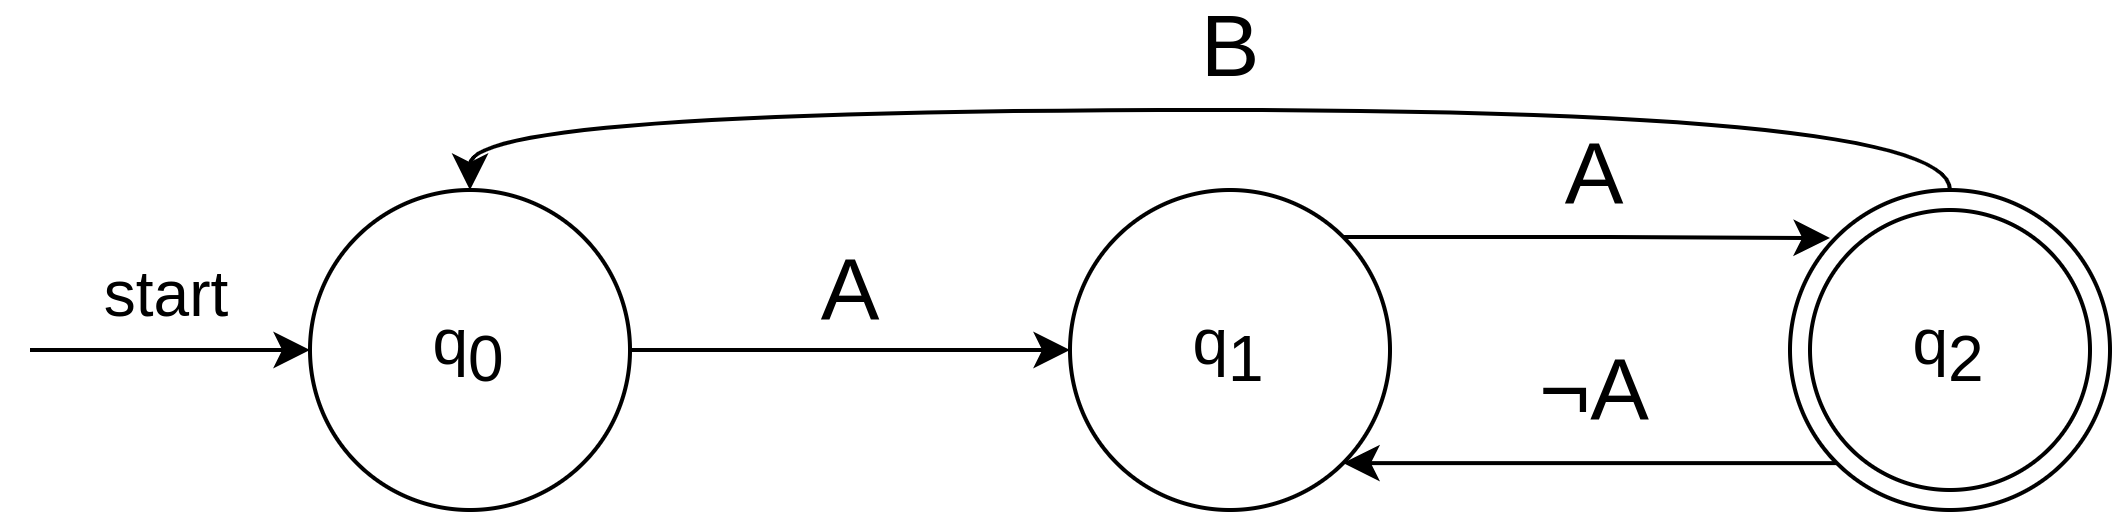
\includegraphics[width=0.8\linewidth]{figures/nba-example.png}
    \caption{Example of NBA accepting any word where every B is preceded by a positive even number of A}
    \label{fig:nba-example}
\end{figure}

There exists a generalization of B{\"u}chi Automata with $n$ acceptance sets of states and the acceptance condition changes as follows: there exists some states that visit each acceptance set of states infinitely many times. It is always possible to compile a Generalized B{\"u}chi Automaton to a Non-deterministic B{\"u}chi Automaton, but GBAs are easier to be used in many cases, like some model checking algorithms.

\begin{definition}[\cite{gastin-oddoux-2001} Generalized B{\"u}chi Automata (GBA)]
A Generalized B{\"u}chi Automata $\automaton$ is a tuple $\automaton = \tuple{\Sigma,Q,I,\delta,\set{F_1,\dots,F_n}}$ where $\Sigma$, $Q$, $I$ and $\delta$ have the same definition of a NBA, but there are $n$ acceptance sets of states $F_1,\dots,F_n$ such that $F_i \subseteq Q$ for all $i \in [1,n]$.
\end{definition}

\begin{definition}[\cite{gastin-oddoux-2001} Run and Language of a GBA]
Let $\automaton = \tuple{\Sigma,Q,I,\sigma,\set{F_1,\dots,F_n}}$ be a GBA and $\sigma = \sequence{\sigma_0,\sigma_1} \in \Sigma^{w}$ be a $\omega$-word over $\Sigma$.
A run of $\automaton$ over $\sigma$ is an infinite sequence of states $\tau = \sequence{q_0,q_1,\dots} \in Q^w$ such that $q_0 \in I$ and $\tuple{q_i,\sigma_i,q_{i+1}} \in \delta$, for each $i \in [0,n]$.
We say that $\tau$ is accepting if and only if for each acceptance set of states $F \in \set{F_1,\dots,F_n}$ there exists a state $q_i \in F$ for infinitely many $i \in \Nat$.
A $\omega$-word $\sigma$ is accepted by $\automaton$ if and only if there exist an accepting run of $\automaton$ over $\sigma$. 
The language accepted by $\automaton$, denoted as $\lang{\automaton}$, is the set of all and only the $\omega$-words $\sigma \in \Sigma^\omega$ accepted by $\automaton$.
\end{definition}

Two important classes of $\omega$-regular languages comprise those languages that express the fact that something bad never happens, called safety languages, and those languages that express that fact that something good eventually happens, called co-safety languages.
The class of the $\omega$-regular co-safety languages coSAFETY is defined as the dual of SAFETY, that is the set of languages $\omegalang{}$ such that $\omegalang{} \in coSAFETY$ iff $\bar{\omegalang{}} \in SAFETY$, where $\bar{\omegalang{}}$ is the complement language of $\omegalang{}$.

\begin{definition}[\cite{geatti-2021-09} Safety languages]
Let $\omegalang{} \subseteq \Sigma^\omega$ be an $\omega$-regular language. We say that $\omegalang{}$ is a safety language if and only if for all words $\sigma \in \Sigma^\omega$ it holds that, if $\sigma \not\in \lang{}$, then $\exists i \in \Nat .\; \forall \sigma' \in \Sigma^\omega .\; \sigma_{[0,i]} \cdot \sigma' \not\in \lang{}$. We call $\sigma_{[0,i]}$ a bad-prefix since it leads to a state where a word can not be in the language no matter how it is going to evolve.
The class of safety $\omega$-regular languages is denoted as SAFETY.
\end{definition}

\begin{definition}[\cite{geatti-2021-09} Co-safety languages]
Let $\omegalang{} \subseteq \Sigma^\omega$ be a $\omega$-regular language. We say that $\omegalang{}$ is a co-safety language if and only if for all words $\sigma \in \Sigma^\omega$ it holds that, if $\sigma \in \lang{}$, then $\exists i \in \Nat .\; \forall \sigma' \in \Sigma^\omega .\; \sigma_{[0,i]} \cdot \sigma' \in \lang{}$. We call $\sigma_{[0,i]}$ a good-prefix since it leads to a state where a word is in the language no matter how it is going to evolve.
The class of co-safety $\omega$-regular languages is denoted as coSAFETY.
\end{definition}

Since each $\omega$-regular language is recognized by a NBA, it is easy to see that we could categorize all automata accepting safety languages. This type of automata is called Safety Automata and are used a lot in my thesis, so let me state them.

\begin{definition}[\cite{gastin-oddoux-2001} Safety Automata (NSA and DSA)]
A Non-deterministic Safety Automata is a tuple $\automaton = \tuple{\Sigma,Q,I,\delta}$, where: (i) $\Sigma$ is a finite alphabet; (ii) $Q$ is a finite set of states; (iii) $I \subseteq Q$ is the set of initial states; (iv) $\delta \subseteq Q \times \Sigma \times Q$ is the transition relation.
If $\delta$ is a partial function $\delta \colon Q \times \Sigma \to Q$, we say that $\automaton$ is a Deterministic Safety Automata (NSA). 
\end{definition}

\begin{definition}[\cite{gastin-oddoux-2001} Run and Language of a NSA]
Let $\automaton = \tuple{\Sigma,Q,I,\sigma}$ be a NSA and $\sigma = \sequence{\sigma_0,\sigma_1} \in \Sigma^{w}$ be a $\omega$-word over $\Sigma$.
A run of $\automaton$ over $\sigma$ is an infinite sequence of states $\tau = \sequence{q_0,q_1,\dots} \in Q^w$ such that $q_0 \in I$ and $\tuple{q_i,\sigma_i,q_{i+1}} \in \delta$, for each $i \in [0,n]$.
A $\omega$-word $\sigma$ is accepted by $\automaton$ if and only if there exist a run of $\automaton$ over $\sigma$. 
The language accepted by $\automaton$, denoted as $\omegalang{(\automaton)}$, is the set of all and only the $\omega$-words $\sigma \in \Sigma^\omega$ accepted by $\automaton$.
\end{definition}

It is simple to see that the language recognized by any safety automaton is a safety language, since the only way for a $\omega$-word to be rejected by a safety automaton is to induce a run that at some point gets stuck, i.e. it can not continue to any state reading the current letter. This implies that a $\omega$-word rejected by a safety automaton is rejected in a finite number of steps, inducing a bad-prefix.  

\begin{theorem}
Given $\omegalang{}$ a language over infinite words, $\omegalang{} \in SAFETY$ if and only if $\omegalang{}$ is recognized by some NSA.
\end{theorem}

%!TEX root = ../../main.tex

\section{Linear Temporal Logic}

After a brief introduction to B{\"u}chi Automata and $\omega$-regular languages, concede us to jump to the logic world with Linear Temporal Logic.

Linear Temporal Logic ($\ltl$) is a modal logic interpreted over infinite, discrete and linear ordered time. $\ltl$ can be seen as an extension of propositional logic with the addition of the \textit{next} operator ($\ltlX{\phi}$, i.e. at the next state $\phi$ holds) and the \textit{until} operator ($\ltlU{\phi_1}{\phi_2}$, i.e. $\phi_2$ will eventually hold and $\phi_1$ will hold until then).

\begin{definition}[\cite{geatti-2021-09} The logic $\ltl$]
Let $\Sigma$ be a set of propositions, $\ltl$ formulas are inductively defined as follows:
\begin{flalign*}
\phi := p \; | \; \ltlNeg{\phi} \; | \;  \ltlOr{\phi_1}{\phi_2} \; | \; \ltlX{\phi} \; | \; \ltlU{\phi_1}{\phi_2}
\end{flalign*}
where $p \in \Sigma$.
\end{definition}

Linear temporal logic with Past ($\pastltl$) extends $\ltl$ with the addition of temporal operators that can talk about the past, and it is obtained from $\ltl$ by adding the following past temporal operators: the $\textit{yesterday}$ operator ($\ltlY{\phi}$, i.e. there exists a previous state in which $\phi$ holds); the \textit{weak yesterday} operator ($\ltlZ{\phi}$, i.e. either a previous state does not exist or in the previous state $\phi$ holds); the \textit{since} operator ($\ltlS{\phi_1}{\phi_2}$, i.e. there was a past state where $\phi_2$ held and $\phi_1$ has held since then). 

\begin{definition}[ \cite{geatti-2021-09} The logic $LTL+P$]
Let $\Sigma$ be a set of propositions, $LTL+P$ formulas are inductively defined as follows:
\begin{flalign*}
\phi := p \; &| \; \ltlNeg{\phi} \; | \;  \ltlOr{\phi_1}{\phi_2} \; | \; \ltlAnd{\phi_1}{\phi_2}
\tag{propositional connectives}\\
&|\; \ltlX{\phi} \; | \; \ltlU{\phi_1}{\phi_2} \;
\tag{future temporal operators} \\
&| \; \ltlY{\phi} \; | \; \ltlZ{\phi} \; | \; \ltlS{\phi_1}{\phi_2}
\tag{past temporal operators} \\
\end{flalign*}
where $p \in \Sigma$.
\end{definition}

To simplify writing of formulas, we define following abbreviations:
\begin{enumerate}[label=\roman*.]
    \item true: $\ltlTrue \equiv \ltlOr{\phi}{\ltlNeg{\phi}}$; false: $\ltlFalse \equiv \ltlAnd{\phi}{\ltlNeg{\phi}}$; implication: $\ltlImpl{\phi_1}{\phi_2} \equiv \ltlOr{\ltlNeg{\phi_1}}{\phi_2}$; iff: $\ltlIff{\phi_1}{\phi_2} \equiv \ltlAnd{\ltlImpl{\phi_1}{\phi_2}}{\ltlImpl{\phi_2}{\phi_1}}$;
    \item $\ltlXexp{\phi}{i}$ is $\ltlX{\ltlXexp{\phi}{i-1}}$ if $i > 0$ and $\phi$ if $i=0$;
    \item release: $\ltlR{\phi_1}{\phi_2} \equiv \ltlNeg{(\ltlU{\ltlNeg{\phi_1}}{\ltlNeg{\phi_2}})}$, i.e. either $\phi_2$ is always true, or it will happen that $\phi_1$ is true and in the meantime $\phi_2$ is always true; 
    \item eventually: $\ltlF{\phi} \equiv \ltlU{T}{\phi}$, i.e. $\phi$ will be true eventually;
    \item globally: $\ltlG{\phi} \equiv \ltlNeg{\ltlF{\ltlNeg{\phi}}}$, or $\ltlG{\phi} \equiv \ltlR{\ltlFalse}{\phi}$, i.e. $\phi$ is always true;
    \item trigger: $\ltlT{\phi_1}{\phi_2} \equiv \ltlNeg{(\ltlS{\ltlNeg{\phi_1}}{\ltlNeg{\phi_2}})}$, i.e. either $\phi_2$ was always true in the past, or it is happened that $\phi_1$ was true and in the meantime $\phi_2$ was always true;
    \item once: $\ltlO{\phi} \equiv \ltlS{\ltlTrue}{\phi}$, i.e. $\phi$ was true at least one time in the past; 
    \item historically: $\ltlH{\phi} \equiv \ltlNeg{\ltlO{\ltlNeg{\phi}}}$, i.e. $\phi$ was always true in the past.
\end{enumerate}

We can even make a further distinction starting from $\pastltl$. We say that a $\pastltl$ formula is \textit{pure past} if and only if all temporal operators inside the formula are past operators.
\textit{Full Past LTL} ($\fpltl$) is the fragment of $LTL+P$ that only admits past operators.

Formulas from $\pastltl$ are interpreted over state sequences. A \textit{state sequence} $\sigma = \sequence{\sigma_0,\sigma_1,\dots}$ is an infinite, linearly ordered sequence of states, where each state $\sigma_i$ is a set of proposition letters, that is $\sigma_i \in 2^\Sigma$ for $i \in \Nat$. Given two indices $i,j \in \Nat$ with $i \leq j$, we denote as $\sigma_{[i,j]}$ the interval of $\sigma$ from index $i$ to $j$, that is $\langle \sigma_i,\dots,\sigma_j \rangle$.

To be more precise, let us formalize the semantics of temporal operators we have seen so far plus some additional abbreviations.

\begin{definition}[\cite{geatti-2021-09} $\pastltl$ semantics]
A state-sequence is an infinite sequence $\sigma = \sequence{\sigma_0,\sigma_1,\dots} \in (2^\Sigma)^\omega$ of sets of propositions $\sigma_i \in 2^\Sigma$.
Given a sequence $\sigma$, a position $i\geq 0$ and a formula $\phi$, the satisfaction of $\phi$ by $\sigma$ at $i$, written $\sigma,i \models \phi$, is inductively defined as follows:
\begin{flalign*}
&\sigma,i \models p             &\iff& & & p \in \sigma_i \\
&\sigma,i \models \ltlNeg{\phi} &\iff& & & \sigma,i \not\models \phi \\
&\sigma,i \models \ltlOr{\phi_1}{\phi_2} &\iff& & & \text{$\sigma,i \models \phi_1$ or $\sigma,i \models \phi_2$} \\
&\sigma,i \models \ltlAnd{\phi_1}{\phi_2} &\iff& & & \text{$\sigma,i \models \phi_1$ and $\sigma,i \models \phi_2$} \\
&\sigma,i \models \ltlX{\phi} &\iff& & & \sigma,i+1 \models \phi \\
&\sigma,i \models \ltlY{\phi} &\iff& & & \text{$i>0$ and $\sigma,i-1 \models \phi$} \\
&\sigma,i \models \ltlZ{\phi} &\iff& & & \text{$i=0$ or $\sigma,i-1 \models \phi$} \\
&\sigma,i \models \ltlU{\phi_1}{\phi_2} &\iff& & & \text{$\exists j \geq i$ such that $\sigma,j \models \phi_2$ and} \\
& & & & & \text{$\sigma,k\models \phi_1$ for all $i \leq k < j$} \\
&\sigma,i \models \ltlR{\phi_1}{\phi_2} &\iff& & & \text{either for all $j \geq i$ such that $\sigma,j \models \phi_2$,} \\
& & & & & \text{or $\exists j \geq i$ such that $\sigma,j \models \phi_1$ and} \\
& & & & & \text{$\sigma,k\models \phi_1$ for all $i \leq k \leq j$} \\
&\sigma,i \models \ltlS{\phi_1}{\phi_2} &\iff&&& \text{$\exists j \leq i$ such that $\sigma,j \models \phi_2$ and} \\
& & & & & \text{$\sigma,k\models \phi_1$ for all $j < k \leq i$}
\end{flalign*}
\end{definition}

We say that $\sigma$ satisfies $\phi$, written $\sigma \models \phi$, if and only if $\sigma,0 \models \phi$. In this case we call $\sigma$ a model of $\phi$.

$\ltl$ can also be enriched with bounded temporal operators, such as the \textit{bounded until} $\ltlUbounded{\phi_1}{\phi_2}{[a,b]}$, \textit{bounded eventually} $\ltlFbounded{\phi}{[a,b]} \equiv \ltlUbounded{\ltlTrue}{\phi_2}{[a,b]}$ and \textit{bounded globally} $\ltlGbounded{\phi}{[a,b]} \equiv \ltlNeg{\ltlFbounded{\ltlNeg{\phi}}{[a,b]}}$. We define the bounded until operator as a shortcut for the $\ltl$ formula $\bigvee_{i=a}^{b}(\ltlXexp{\psi_2}{i}\land \bigwedge_{j=0}^{i-1}\ltlXexp{\psi_1}{j})$.
\textit{Full Bounded LTL} ($\fbltl$) is the fragment of LTL that includes only the next and bounded eventually operators.

\textit{Extended Bounded Response LTL} ($\ebrltl$) extends $LTL_{FB}$ by admitting Boolean combinations of the universal unbounded temporal operators release ($\ltlR{}{}$) and globally ($\ltlG{}$).
If we allow using past operators in $\ebrltl$, then we get the $\pastebrltl$ which is defined as follows.

\begin{definition}[\cite{geatti-2020-08} The logic $\ebrltl$]
Let $a,b \in \Nat$. A $\ebrltl$ formula $\chi$ is inductively defined as follows:
\begin{flalign}
&\psi := p \; | \; 
        \ltlNeg{\psi} \; | \; 
        \ltlOr{\psi_1}{\psi_2} \; | \; 
        \ltlX{\psi} \; | \;
        \ltlUbounded{\psi_1}{\psi_2}{[a,b]}
        \tag{Bounded Future Layer} \\
&\phi := \psi \; | \; 
        \ltlAnd{\phi_1}{\phi_2} \; | \; 
        \ltlX{\phi} \; | \; 
        \ltlG{\phi} \; | \; 
        \ltlR{\psi}{\phi}
        \tag{Future Layer} \\
&\chi := \phi \; | \; 
        \ltlOr{\chi_1}{\chi_2} \; | \; 
        \ltlAnd{\chi_1}{\chi_2}
        \tag{Boolean Layer}
\end{flalign}
\end{definition}


\begin{definition}[\cite{geatti-2021-09} The logic $\pastebrltl$]
Let $a,b \in \Nat$, a $\pastebrltl$ formula $\chi$ is inductively defined as follows:
\begin{flalign}
&\eta := p \; | \; 
        \ltlNeg{\eta} \; | \;
        \ltlOr{\eta_1}{\eta_2} \; | \;
        \ltlY{\eta} \; | \;
        \ltlS{\eta_1}{\eta_2}
        \tag{Pure Past Layer} \\
&\psi := \eta \; | \; 
        \ltlNeg{\psi} \; | \; 
        \ltlOr{\psi_1}{\psi_2} \; | \; 
        \ltlX{\psi} \; | \;
        \ltlUbounded{\psi_1}{\psi_2}{[a,b]}
        \tag{Bounded Future Layer} \\
&\phi := \psi \; | \; 
        \ltlAnd{\phi_1}{\phi_2} \; | \; 
        \ltlX{\phi} \; | \; 
        \ltlG{\phi} \; | \; 
        \ltlR{\psi}{\phi}
        \tag{Future Layer} \\
&\chi := \phi \; | \; 
        \ltlOr{\chi_1}{\chi_2} \; | \; 
        \ltlAnd{\chi_1}{\chi_2}
        \tag{Boolean Layer}
\end{flalign}
\end{definition}

Before arguing the advantage to add past temporal operators to $\ebrltl$, we introduce the expressiveness of a temporal logic.
The notion of expressiveness of a temporal logic is an extension of the notion of equivalence of formulas.
We say that two formulas $\phi$ and $\psi$ are equivalent ($\phi \equiv \psi$) if and only if they are satisfied by the same set of state sequences.
A temporal logic $\logic$ is said to be at least as expressive as another temporal logic $\logic'$, if for each formula $\phi \in \logic$, there exists a formula $\psi \in \logic'$ such that $\phi \equiv \psi$.
A temporal logic $\logic$ is said to be less expressive than another temporal logic $\logic'$ if, there exists a formula $\phi \in \logic'$ that for each formula $\psi \in \logic$, $\phi \not\equiv \psi$.
Two temporal logic are equally expressive when they are at least as expressive as each other.

In \cite{geatti-2021-09} has been proved that, without past temporal operators, $\ebrltl$ is less expressive than the safety fragment of $\ltl$. However, we achieve the same expressiveness of the safety fragment of $\ltl$ by adding past temporal operators, becoming a safety language at the same level of other more famous LTL dialects, like $\ltlG{\alpha}$, i.e. formulas starting with \textit{globally} and ending with $\alpha$ is a \textit{pure past formula}, and \textit{Safety-LTL}, i.e. formulas of $\ltl$ without \textit{until} temporal operator and in Negation Normal Form (NNF).
Just to give the general idea of the proof of $\semantics{\ebrltl} \subsetneq \semantics{\ltl} \cap SAFETY$, we can show that the formula $\phi_G := \ltlG{(\ltlOr{p_1}{\ltlG{p_2}})}$ belongs syntactically to Safety-LTL, but it is not expressible by any $\ebrltl$ formula. On the contrary, note that $\phi_G$ is expressible in $\pastebrltl$ since $\phi_G := \ltlG{(\ltlOr{p_1}{\ltlG{p_2}})} \equiv \ltlG{(\ltlImpl{\ltlNeg{p_2}}{\ltlH{p_1}})}$.

\begin{theorem}[\cite{geatti-2021-09} Expressiveness of $\ebrltl$]
$\semantics{\ebrltl} \subsetneq \semantics{\ltl} \cap SAFETY$
\end{theorem}

\begin{theorem}[\cite{geatti-2021-09} Expressiveness of $\pastebrltl$]
$\semantics{\pastebrltl} = \semantics{\ltlG{\alpha}} = \semantics{\text{\textit{Safety-LTL}}} =  \semantics{\ltl} \cap SAFETY$
\end{theorem}

\subsection{Temporal Hierarchy}
Safety and Co-safety properties covers only a subset of all properties expressible by Linear Temporal Logic.
LTL formulas can be divided in classes that form a hierarchy, highlighting the relation among their normal forms defined as Boolean and temporal combinations of full-past formulas. For this reason, whenever we write $\alpha_1$, $\alpha_2$ in this sub-section, we mean two full-past formulas ($\alpha_1,\alpha_2 \in \fpltl$).
Such hierarchy is called Temporal Hierarchy and it was introduced by Manna and Pnueli \cite{pnueli1990}.

Previously we have seen two important type of classes, which are at base of the hierarchy: safety and co-safety properties. 
Safety properties express the fact that "something bad will never happen". An important type of safety properties are invariant properties, which are boolean propositions that must always hold. 
Safety properties are expressible by full-past formulas preceded by a globally operator ($\ltlG{\alpha}$).
Co-safety properties the fact that "a good thing will happen at least one time" and they are expressible by full-past formulas preceded by an eventually operator ($\ltlF{\alpha}$).

The next class of $\ltl$ properties is called obligation class and consists in Boolean combinations of the two classes defined above. 
Its name derived from the fact that its properties impose a conditional obligation ($\ltlOr{\ltlG{\alpha_1}}{\ltlF{\alpha_2}} \equiv \ltlImpl{\ltlF{\alpha_1'}}{\ltlF{\alpha_2}}$ with $\alpha_1' \equiv \ltlNeg{\alpha_1}$), where if something happens, then something else will happen. The normal form of the obligation class is the set of formulas of type $\bigwedge_{i=1}^n(\ltlOr{\ltlG{\alpha_1}}{\ltlF{\alpha_2}})$ for some $n \in \Nat$.

Another formulation for the previous class is the intersection of two other important classes: liveness and persistence. 
\textit{Liveness} expresses properties of type "a good thing will happen infinitely many times" and they are described by formulas of type $\ltlG{\ltlF{\alpha}}$. 
\textit{Persistence} expresses properties of type "a good thing will constantly happen from a certain point on and they are described by formulas of type $\ltlF{\ltlG{\alpha}}$.

Considering the Boolean combinations of liveness and persistence properties, we end up with the reactivity class. A \textit{reactivity} property, like an obligation property, expresses a conditional obligation of the type "if a good thing happens infinitely many times, so does another thing". The normal form of this class comprises all formulas of type $\bigwedge_{i=1}^{n}(\ltlOr{\ltlG{\ltlF{\alpha_1}}}{\ltlF{\ltlG{\alpha_2}}})$, expressible also as $\ltlImpl{\ltlG{\ltlF{\alpha_2'}}}{\ltlG{\ltlF{\alpha_1}}}$ with $\alpha_2' \equiv \ltlNeg{\alpha_2}$, for some $n \in \Nat$. Reactivity class is exactly the set of all $\ltl$ formulas and so they have the same expressiveness.
Actually, there is an entire hierarchy inside the reactivity class, where we define $R(n)$ for some $n \in \Nat$ as the classes of formulas with a fixed number $n$ of conjunctions.
Moreover, it is been proved that $\semantics{R(n)} \subsetneq \semantics{R(n+1)}$ for each $n \in \Nat$.


\begin{figure}[!htp]
    \centering
    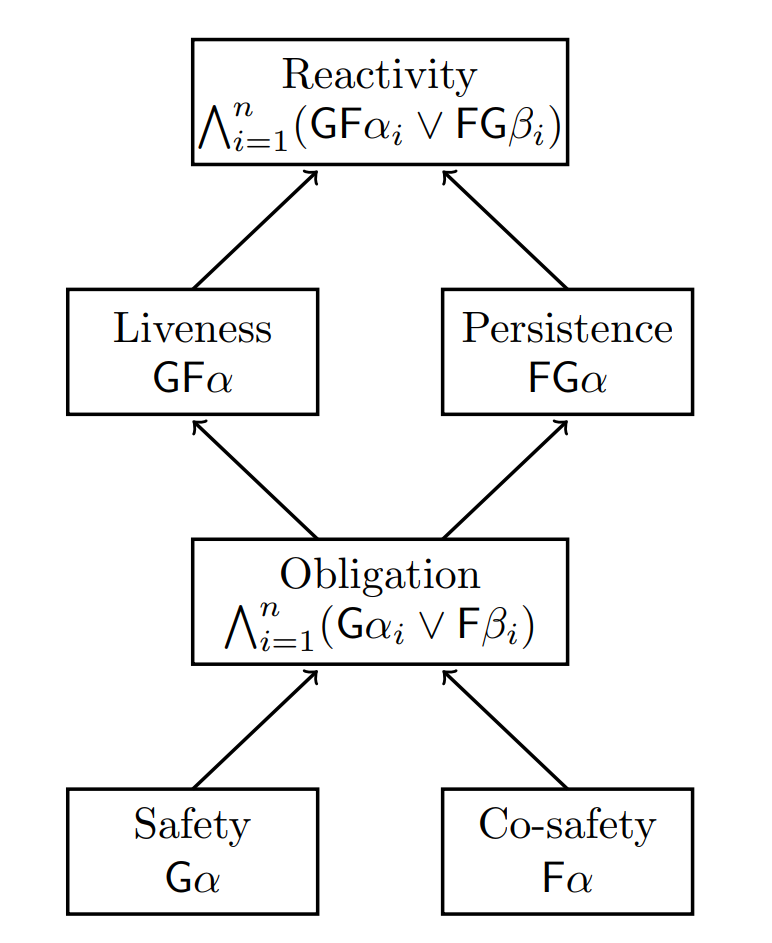
\includegraphics[width=0.4\linewidth]{figures/temporal-hierarchy.png}
    \caption{\cite{pnueli1990} Temporal Hierarchy describing the relation among temporal classes along with their normal forms. The arrows represent the inclusions between the classes.}
    \label{fig:temporal-hierarchy}
\end{figure}

%!TEX root = ../../main.tex

\section{Automaton-based LTL Model Checking}
\label{sec:ltl-model-checking}

In this section we merge B{\"u}chi automata and Linear Temporal Logic, presenting what an abstraction of a system is, the basic idea of Automaton-based LTL Model Checking and some useful definitions for later.
Automaton-based LTL Model Checking is the technique to verify a property $\phi$ expressed in $\ltl$ on a model of a system introduced for the first time by \cite{VW86}. 

Given a system, a model represents an abstraction of it. 
The model of a system is designed as a Transition System (TS), which is a mathematical model to describe the potential behaviour of discrete systems. It consists of states and transitions between states, which may be labeled with labels chosen from a set.
Transition Systems differ from finite-state automata in several ways: the set of states is not necessarily finite, the set of transitions is not necessarily finite and no start and final states are given. 
The most widely used type of Transition Systems is Labeled Transition Systems, which consists of Transition System with an additional labelling function mapping each node with a word over an alphabet $AP$.

Another way to design the model of a system is by Moore Machine or Mealy Machine. Both machines are finite-state machines, but differently from other finite automata that determine the acceptance of a particular string in a given language, they determine the output against given input. The formalization of the two machines is quite the same: a set of states, an initial state, input and output alphabets, a transition function and an output function. They differ only in the output function: in Mealy Machine the output function value depends on the current state and the current input symbol, while in Moore Machine the output function value depends only on the current state.

In this section we use LTS as main model, but we wanted to give the definition of Moore Machine and Mealy Machine since we are going to cite them in later chapters.

\begin{definition}[\cite{principles-cps} Labeled Transition System (LTS)]
A Labeled Transition System is a tuple $\model = \tuple{S, \to, I, AP, L}$ consisting of: (i) a finite set $S$ of states; (ii) a transition relation $\to \subseteq S \times S$; (iii) a set $I \subseteq S$ of initial states; (iv) a set $AP$ of atomic propositions (alphabet); (v) a labeling function $L \colon S \to 2^{AP}$.
\end{definition}

\begin{definition}[\cite{principles-cps} Moore Machine]
A Moore Machine is a tuple $\model = \tuple{S,s_0,I,O,\delta,\lambda}$ consisting of: (i) a finite set $S$ of states; (ii) an initial state $s_0 \in S$; (iii) a finite set called input alphabet; (iv) a finite set called output alphabet; (v) a transition function $\delta \colon S \times I \to S$; (vi) an output function $\lambda \colon S \to O$.
\end{definition}

\begin{definition}[\cite{principles-cps} Mealy Machine]
A Mealy Machine is a tuple $\model = \tuple{S,s_0,I,O,\delta,\lambda}$ consisting of: (i) a finite set $S$ of states; (ii) an initial state $s_0 \in S$; (iii) a finite set called input alphabet; (iv) a finite set called output alphabet; (v) a transition function $\delta \colon S \times I \to S$; (vi) an output function $\lambda \colon S \times I \to O$.
\end{definition}

From a set $s$ in a transition system we can define: the set of direct successors, i.e. the states reachable in one step; the set of direct predecessors, i.e. the states from which $s$ can be reached by one step; the set of states reachable by an undefined number of steps; the set of states from which $s$ can be reached by an undefined number of states; the set of states reachable starting from the initial states.

\begin{definition}[\cite{principles-cps} $Pre$, $Post$ and $reachability$ sets]
Let $\model = \tuple{S, \to, I, AP, L}$ be a Labeled Transition System and a state $s \in S$.
\begin{itemize}
    \item The set $Post(s)$ of direct successors of $s$ is defined by $Post(s) = \set{s' \in S \; | \; s \to s'}$.
    \item The set $Pre(s)$ of direct predecessors of $s$ is defined by $Pre(s) = \set{s' \in S \; | \; s' \to s}$.
    \item The set $Post^*(s)$ consists of the states reachable in the state graph from $s$. Given $C \subseteq S$, the set $Post^*(C)$ is defined by $Post^*(C) = \bigcup_{s \in C} Post^*(s)$.
    \item The set $Pre^*(s)$ consists of the states reachable in the state graph from $s$. Given $C \subseteq S$, the set $Pre^*(C)$ is defined by $Pre^*(C) = \bigcup_{s \in C} Pre^*(s)$.
    \item The set $Reach(TS) = Post^*(I)$ is the reachability set of TS from $I$.
\end{itemize}
\end{definition}

\begin{definition}[\cite{principles-cps} Paths and Traces sets]
Let $\model = \tuple{S, \to, I, AP, L}$ be a Labeled Transition System. 
\begin{itemize}
    \item A finite path fragment is a finite state sequence $\sequence{s_0,s_1,\dots,s_n}$ for some $n\geq 0$ such that $s_i \in Post(s_{i-1})$ for all $i < 0 \leq n$.
    \item An infinite path fragment is an infinite state sequence $\sequence{s_0,s_1,\dots}$ such that $s_i \in Post(s_{i-1})$ for all $i > 0$.
    \item A path fragment is initial if $s_0 \in I$. 
    \item The set $Paths(\model)$ defines all the initial paths of $\model$.
    \item A trace of an infinite path fragment is the sequence of sets of atomic propositions $\sequence{L(s_0), L(s_1), \dots} \in Traces(TS)$.
    \item The set $Traces(\model)$ defines all traces of all paths in $Paths(\model)$.
\end{itemize}
\end{definition}

After having described what a model of a system is, let us go on speaking about properties of a model. 
Given a model $\model$, we want to specify admissible traces. 
This can be done exploiting linear-time (LT) property over the atomic propositions $AP$, that is a subset of $(2^{AP})^\omega$. 
Since linear-time properties are hard to describe, we may need of a logic to describe them in a fancier way. 
Here $\ltl$ comes in play, because it is a logic allowing to describe linear time properties over the atomic proposition $AP$. 
When we speak about linear-time property via $\ltl$, it is useful recognizing the set of words described by $\phi$.

\begin{definition}[\cite{principles-cps} Words of a $\ltl$ formula]
Let $\phi$ be a $\ltl$ formula over $AP$, the set $Words(\phi)$ is defined as all the words where $\phi$ holds, i.e. $Words(\phi) = \set{\sigma \in (2^{AP})^\omega \; | \; \sigma \models \phi}$.
\end{definition}

LTL Model Checking is the task to say whether a formula $\phi$ is satisfied by a model $\model$. If that is case, then yes must be returned, otherwise a counterexample must be returned as the proof of $\model \not\models \phi$.
The underlying idea under Automaton-based LTL Model Checking is to verify whether all traces of $\model$ are subset of word of $\phi$, namely $\model \models \phi \iff Traces(TS) \subseteq Words(\phi)$. 
That is because we can say that $\model \models \phi$ only if $\phi$ holds no matter the trace undertaken by any execution of $\model$. 
Starting from this idea we deduce that we could reason even in a different way, that is there is no path on which the negation of $\phi$ holds. 
If such path exists, then it is a counterexample for $\model \models \phi$.
From here we can also do a next step. Now we are speaking about traces and words, but we can do the same reasoning speaking about automata.
Actually, for each $\ltl$ formula $\phi$ there exists a related automaton such that the language of $\phi$ and the language of such automaton are the same. 
This can be done by converting $\phi$ into a Generalized B{\"u}chi Automaton and then into a Non-deterministic B{\"u}chi Automaton. 
This unlocks the possibility to express the problem using automata. 
To perform Automaton-based LTL Model Checking we need to follow these steps:
\begin{itemize}
    \item construct the B{\"u}chi Automaton $\automaton_{\ltlNeg{\phi}}$ corresponding to the negated specification;
    \item build the product automaton between $\model$ and $\automaton_{\ltlNeg{\phi}}$;
    \item search for accepting cycles in the composition $\model \times \automaton_{\ltlNeg{\phi}}$. If there exists one cycle, then it means that $\ltlNeg{\phi}$ is satisfied, otherwise it means that $\phi$ is satisfied. In other words, we look for a point in the time from which is not possible to visit accepting states infinitely often.
\end{itemize}
Following we can see all previous concepts formally.

\begin{definition}[\cite{principles-cps} Counterexample]
A counterexample $\pi$ of a $\ltl$ formula $\phi$ over a LTS $\model$ is a path (even infinite) such that $\pi \not\models \phi$.
\end{definition}

\begin{theorem}[\cite{VW86}]
For any $\ltl$ formula $\phi$ over $AP$, there exists a NBA $\automaton_{\phi}$ over $2^{AP}$ such that $Words(\phi) = \omegalang{(\automaton_{\phi})}$.
\end{theorem}

\begin{definition}[\cite{principles-cps} Product automaton between LTS and NBA]
Let $\model = \tuple{S, \to, I, AP, L}$ be a LTS and $\automaton = \tuple{Q,\Sigma,\delta,Q_0,F}$ with $\Sigma = 2^{AP}$ and $Q_0 \cap F = \emptyset$. Their product is defined as the transition system $\model \times \automaton = \tuple{S',\to',I',AP',L'}$ where: 
\begin{enumerate}[label=\roman*.]
    \item $S' = S \times Q$;
    \item $\to'$ is defined by 
    \[ \infer{s \to t \land q \xrightarrow{L(t)} p}{\tuple{s,q} \to' \tuple{t,p}} \]
    \item $I' = \set{\tuple{s_0, q} \; | \; s_0 \in I \land \exists q_0 \in Q_0 \; : \; q_0 \xrightarrow{L(s_0)} q}$;
    \item $AP' = Q$; 
    \item $L' \colon S \times Q \to 2^Q$ with $L'(\tuple{s,q}) = {q}$.
\end{enumerate}
\end{definition}

\begin{definition}[Automaton-based $\ltl$ model checking]
We say that $\model$ satisfies $\phi$, denoted as $\model \models \phi$, if for each path $\pi$ of $\model$ it holds that $\pi \models \phi$, i.e. if $Traces(\model) \subseteq Words(\phi)$.
Equivalently, $\model \models \phi$ if and only if there does not exist a path $\pi$ such that $\model \models \ltlNeg{\phi}$. If such path $\phi$ exists, it is a counterexample for $\model$ over $\phi$. More formally:
\begin{flalign*}
\model \models \phi & \iff Traces(\model) \subseteq Words(\phi) \\
                    & \iff Traces(\model) \subseteq ((2^{AP})^\omega \setminus Words(\phi)) = \emptyset \\
                    & \iff Traces(\model) \cap Words(\phi) = \emptyset \\
                    & \iff Traces(\model) \cap Words(\automaton_{\ltlNeg{\phi}}) = \emptyset \\
                    & \iff \model \times \automaton_{\ltlNeg{\phi}} \models \ltlF{\ltlG{(\ltlNeg{F})}}
\end{flalign*}
where $F$ is the set of accepting states of $\automaton_{\ltlNeg{\phi}}$ and $\model \times \automaton_{\ltlNeg{\phi}}$ is the product automata between LTS and NBA.
\end{definition}

As we have already said in the previous section, an invariant property is a Boolean expression which must hold forever.
The invariant model checking problem, also called invariant verification, is the problem to check whether the Boolean expression holds in all reachable states of the model.

\begin{definition}[Invariant model checking]
We say that $\model$ satisfies $\phi$ invariant property, denoted as $\model \models_{inv} \phi$, if and only if at any position $i$ of any reachable state $s$, it holds $s_i \models \phi$.
\end{definition}

If we consider safety properties, we can reduce their model checking problem to invariant verification \cite{KV99}.
When we negate a safety property, we end up having a co-safety property for which it is enough to find a finite-trace satisfying it. Such finite trace is called informative prefix because it falsifies the original safety property.
The idea behind this method is to provide an automaton of the negated formula and an invariant property on $\phi$ such that all paths falsifying the invariant property on the synchronous product between model and such automaton are informative prefixes (bad-prexifes) of the safety formula. 
Invariant verification is more efficient than usual Automaton-Based LTL model checking and so it is convenient to make this reduction.

\begin{theorem}[\cite{KV99} Invariant verification from safety properties]
We say that $\model$ satisfies $\phi$ safety property, denoted as $\model \models \phi$, if and only if
\begin{flalign*}
\model \models \phi \iff \model \times \automaton_{\ltlNeg{\phi}}^{saf} \models_{inv} \neg F
\end{flalign*}
where $F$ is the set of accepting states of $\automaton_{\ltlNeg{\phi}}$
\end{theorem}

Another problem related to model checking is parameter synthesis in parametric systems.
Parametric systems arise in many application domains from real-time systems to software to cyber-physical systems. In these applications, the system is often part of a larger environment and the designer has to define the system relative to some unknown parameters of the environment. The use of parameters is fundamental in the early phases of the development gibing the possibility to explore different design choices.
A key challenge for the design of parametric systems is the estimation of the parameter valuations that guarantee the correct behaviour of the system.
Manual estimation of these values is time consuming therefore a fundamental problem is to automatically synthesize the maximal region of parameter valuations for which the system satisfies some properties. In \cite{CGMT13} is presented an approach to solve parameter synthesis with the algorithm IC3, one of the major recent breakthroughs in SAT-bases model checking and lately extended to the SMT case.
We will not delve into this topic further, but we will use this technique later.

Before going on to the next section, we would like to introduce an important concept about models.
In practical applications, the model of a system is not given as single block, but it is common to have two split models: one for the plant ($P$) and another for the controller ($C$).
The model checking procedure is performed on their closed-loop $P \times C$, that is their synchronous composition where the output value of plant is sent in input to the controller and the controller output is sent in input to the plant.
This type of modelling is widely used and it is useful to split the behavioural logic (controller) from the actual system (plant). 
Basically, plant defined the constraints of the system while controller reads the current state of the system and determine its next state. 

%!TEX root = ../../main.tex

\section{Reduced Ordered Binary Decision Diagram} \label{sec:robdd}

In real-world cases, exploiting basic model checking algorithms is impossible due to the large amount of states to handle. 
In order to make them usable, we need adapt them by using Binary Decision Diagram which allows to represent and manipulate set of states, also called symbolic representation. 
They have been especially effective as algorithmic basis for symbolic model checkers.

Binary Decision Diagram (BDD) provides a data structure to represent and manipulate Boolean functions symbolically.
The Boolean formulas represented by BDDs are in If-then-else Normal Form (INF), that is a normal form where a formula can be either true, false or a if-then-else expression where the condition is a variable and the branches are formulas in INF. 
Another exploited tool is Shannon's expansion, useful to expand any Boolean functions. 
In our context, the expansion is interpreted as a if-then-else expression, where the condition is a variable $x$ and the co-factors being the branches.

\begin{definition}[If-then-else Normal Form (INF)]
The set of Boolean expressions in If-then-else Normal Form is defined by
\begin{flalign*}
t ::= 0 \; | \; 1 \; | \; x \to t_1,t_2 
\end{flalign*}
where $x$ is a variable.
\end{definition}

\begin{theorem}[\cite{principles-cps} Shannon's expansion]
For every Boolean expression $t$ and a variable $x$, $t \equiv x \to t[1/x],t[0/x]$.
Equivalently, we can express $t$ as $t \equiv (x \land t[1/x]) \lor (\neg x \land t[0/x]$ without using the if-then-else expression. Note that if $t$ has $k$ variables, then the two co-factors have $k-1$ variables.
\end{theorem}

Boolean expressions in INF can be viewed as binary graph known as decision diagram. Each internal node $v$ is labelled with a variable, retrievable by $var(v)$, and has two out-going edges: $low(v)$ to get the sub-tree root related to the negative co-factor and $high(v)$ to get the sub-tree root related to the positive co-factor.
There are three types of BDDs and one is the previous one but with a further condition. 
The first type is BDD, which is built by recursively applying Shannon's expansion on the branches until the branches has no variables. 
Note that BDD type impose no further rules, but it is just the diagram obtained by such procedure. 
One of the biggest issue with BDD is the non-canonicity, that is there could be two or more BDDs representing the same formula.
For this reason we require a BDD to be ordered, that is each sub-tree respects a linear ordering known a-priori. 
Then, to finally reach canonicity we require an Ordered BDD to be reduced, i.e. all nodes are unique (there are no two nodes such that they have the same variable, low and high values) and there are no redundancies (there are no nodes such that its low and high values are equals, and so it's useful). 
The chosen linear-ordering is very important because it could affect the size of the final ROBDD a lot.

\begin{definition}[\cite{principles-cps} Binary Decision Diagram (BDD)]
A BDD is a rooted and directed acyclic graph with: 
\begin{itemize}
    \item all non-terminals labelled with a Boolean variable;
    \item all terminals labelled with $0$ or $1$;
    \item all edged are labelled $0$ or $1$;
    \item all other internal nodes have out-degree two, with one outgoing edge called the low edge and the other called the high edge and are labelled with a variable. The two outgoing edges are given by two functions $low(u)$ and $high(u)$. 
\end{itemize}
\end{definition}

\begin{definition}[\cite{principles-cps} Ordered BDD (OBDD)]
A BDD is ordered if on all paths through the graph the variables respect a given linear order $x_1 < x_2 < \dots < x_n$.
\end{definition}

\begin{definition}[\cite{principles-cps} Reduced OBDD (ROBDD)]
A Ordered BDD is reduced if it's: unique, i.e. no two distinct internal nodes $u$ and $v$ have the same variable, low and high successor; non-redundant, i.e. no internal node $u$ has identical low and high successor.
\end{definition}

\begin{proposition}[\cite{principles-cps} Canonicity of ROBDD]
For a Boolean expression $t$ with variables $x_1 \dots x_n$ and a linear order $x_1 < \dots < x_n$, there exists a unique ROBDD that is equivalent to t.
\end{proposition}

\begin{figure}[!htp]
    \centering
    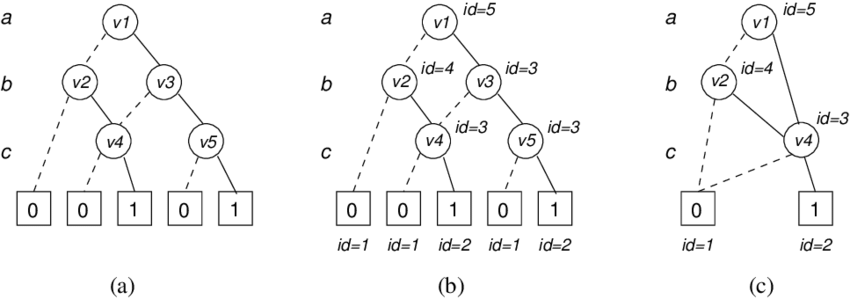
\includegraphics[width=0.8\linewidth]{figures/robdd-example.png}
    \caption{\cite{dhiraj-2023} Example of ROBDD construction for $f=(a \lor b) \land c$; a) OBDD for the variable order a,b,c; b) OBDD with unique identifiers; c) ROBDD for variable order a, b, c.}
    \label{fig:robdd-construction-example}
\end{figure}

From now on whenever it is written BDD, we mean ROBBD, because ROBDD are the only type of BDDs exploited in both practice and theory.
Since BDDs represent Boolean formulas, on them can be applied the common Boolean operations.
Given two BDDs $B_0$ and $B_1$ and denoting with $f(B_0)$ and $f(B_1)$ the two formulas represented by the two BDDs, the common Boolean operations that can be applied on them are:
\begin{itemize}
    \item $and(B_0,B_1)$, returning the ROBDD for the formula $f(B_0) \land f(B_1)$;
    \item $or(B_0,B_1)$, returning the ROBDD for the formula $f(B_0) \lor f(B_1)$;
    \item $not(B_0)$, returning the ROBDD for the formula $\neg f(B_0)$;
    \item $diff(B_0,B_1)$, returning the ROBDD for the formula $f(B_0) \land \neg f(B_1)$;
    \item $exists(B_0,X)$, returning the ROBDD for the formula $\exists X.f(B_0)$;
    \item $forall(B_0,X)$, returning the ROBDD for the formula $\forall X.f(B_0)$;
    \item $rename(B_0,X,Y)$, returning the ROBDD obtained by renaming variables in $X$ to $Y$;
    \item $restrict(B_0,X,1)$ and $restrict(B_0,X,0)$, returning the ROBDD for the formula $f(B_0)[1/X]$ and $f(B_0)[0/X]$, respectively the positive and negative co-factors.
\end{itemize} 

The complexity of each of the above operations is $O(\card{B_0})$ for unary ones and $O(\card{B_0} \cdot \card{B_1})$ for binary ones, with $\card{B}$ meaning the number of nodes of a given BDD $B$.

In order to apply BDDs to model checking, we need to interpret the whole state machine and sets of states as Boolean variables or Boolean formulas .

%!TEX root = ../../main.tex

\section{The AIGER format}

This section presents an important format highly used in model checking and reactive synthesis: AIGER. 

The AIGER format is used to describe circuits by multi-rooted And-Inverter Graphs (AIG) with latches that store the system state. It was developed as a compact and simple file format benchmarks for the hardware model checking competition (HWMCC). 
A And-Inverter Graph is a directed, acyclic graph that represents a structural implementation of the logical functionality of a circuit or network. An AIG consists of two-input nodes representing logical conjunction, terminal nodes labeled with variable names and edges optionally containing markers indicating logical negation. This representation of a logic function is rarely structurally efficient for large circuits, but is an efficient representation for the manipulation of Boolean functions.
Conversion from the network of logic gates to AIGs is fast and scalable. It only requires that every gate be expressed in terms of AND and NOT gates.
This conversion does not lead to unpredictable increase in memory use and runtime. This makes AIG an efficient representation in comparison with either the binary decision diagram (BDD) or the sum-of-product ($\Sigma o \Pi$) form.

% TODO: example of aig?

A file in AIGER format (ASCII variant) consists of the following parts: header, input definitions, latch definitions, output definitions and and-gate definitions. The header consists of a single line \lstinline{aag M I L O A}, where \lstinline{M} gives the maximum variable index, \lstinline{I} the number of inputs, \lstinline{L} the number of latches, \lstinline{O} the number of outputs and \lstinline{A} the number of AND gates.
Boolean variables are referred by even numbers, while odd numbers are referred to the negation of a variable, i.e. if $n$ is even, $n+1$ is the negation of $n$. $0$ and $1$ are special indexes referring the false and true values, respectively.
Then, the format can be divided in 5 sections declared in the header.

\begin{lstlisting}[caption=The empty circuit without inputs nor outputs and constant false/true in AIGER format]
aag 0 0 0 0 0             header

aag 0 0 0 1 0             header
    0                     output

aag 0 0 0 1 0             header
    1                     output
\end{lstlisting}

Every input definition takes one line and consists of a single even number.
Every latch definition takes one line and consists of an even number, followed by a number that defines which variable is used to update the latch in every step. The initial value is given by an additional number between either 0, 1 or the latch itself, which means to set the initial value to false, true or undefined, respectively. By default latches are assumed to have initial value 0.
Every output definition takes one line and consists of a single number, representing a possibly negated input, latch or and-gate. 
Every and-gate definition takes one line and consists of three numbers. The first is an even number, representing the output of the and-gate, and is followed by two numbers representing its (possibly negated) inputs.
There are also two further optional sections: symbol table and comments. The symbol table assigns names to inputs, latches and outputs. It is optional, and need not be complete. Every line defines the name of one input, latch, or output, and starts with i, l, o, respectively,
followed by the number of the input, latch, or output in the sequence of definitions.

As notable example we want to show how to encode a full-adder in AIGER format. A full-adder needs no presentation, it is just a circuits which sum two bits considering the carry.
Usually, a full-adder has three inputs: the two addends and the carry of the previous sum. That's because a full-adder is designed to be chained to other full-adders in order to sum sequence of bits. 
The first full-adder has carry value set to false, while the $i$ full-adder has the carry value in input set to the $i-1$ full-adder carry output. 
In our example, the full-adder is designed to be used as a stand-alone circuit where the carry result is saved in a latch and is used in the next computation, and it is $0$ initially.
Basically, this design choice was made just to show how to encode latches in AIGER format.

\begin{figure}[!htp]
    \centering
    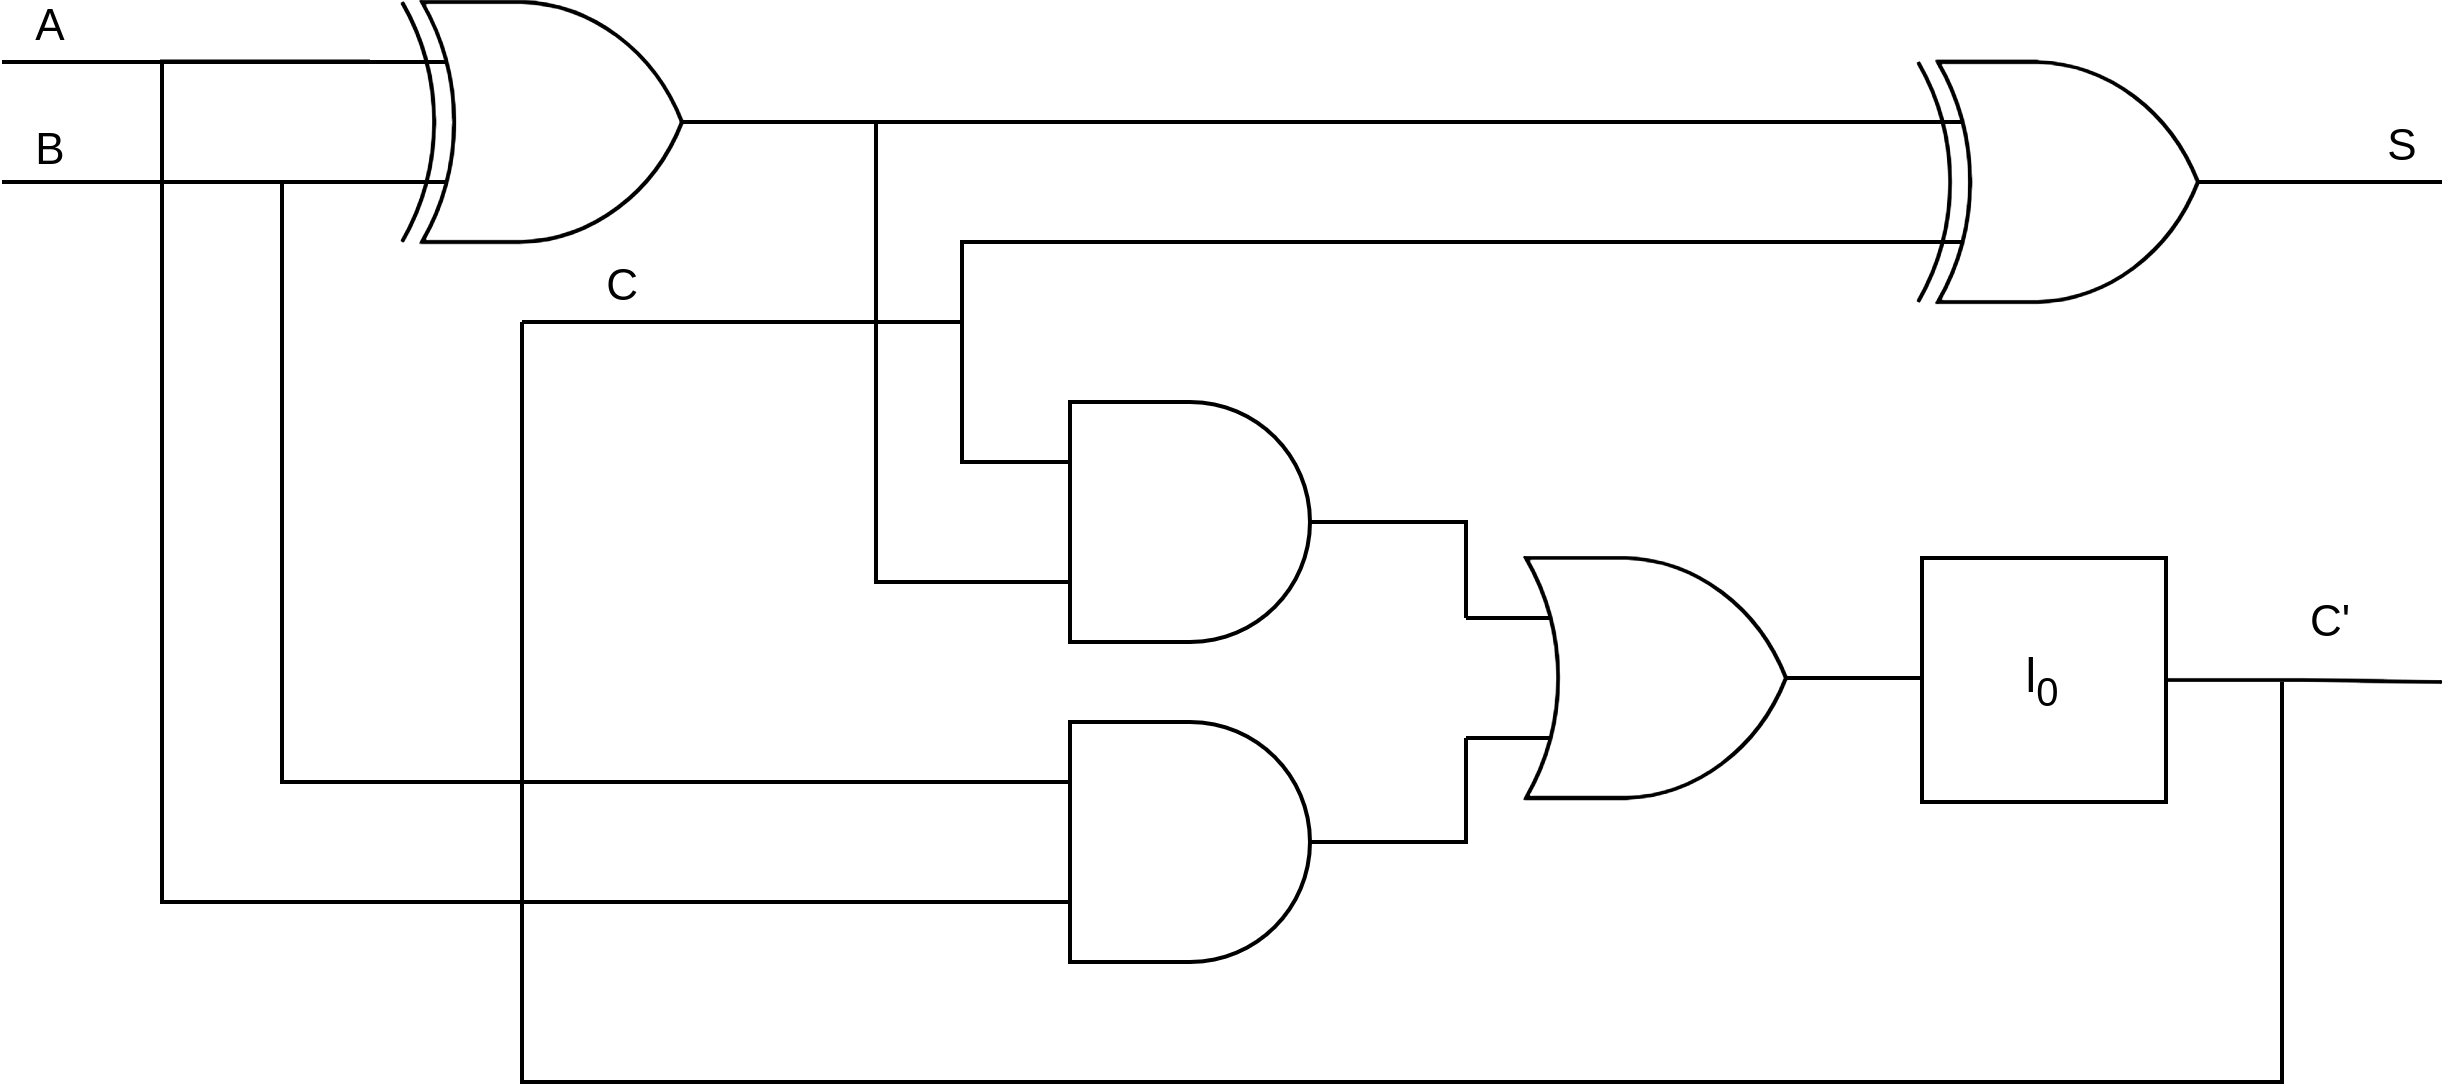
\includegraphics[width=0.6\linewidth]{figures/full-adder-circuit.png}
    \caption{Full adder circuit}
    \label{fig:full-adder-circuit}
\end{figure}

To encode a full-adder we have to express two formulas by just using and and not gates: the sum result and the carry result.
The sum result is given by $S = (A \oplus B) \oplus C$, while the carry result $C' = (A \land B) \lor (C \land (A \oplus B))$. $A$, $B$ are the input bits and $C$ the carry value.
The first step is to convert the formula to Conjunctive Normal Form (CNF) and then remove the or gates by De Morgan's laws. 

\begin{figure}
    \centering
\begin{flalign*}
& (A \oplus B) \oplus C \\
& \iff \text{(by CNF)} \\
& (\neg A \lor \neg B \lor C) \land (\neg A \lor B \lor \neg C) \land (A \lor \neg B \lor \neg C) \land (A \lor B \lor C) \\
& \iff \text{(by De morgan's laws)} \\
& \neg(A \land B \land \neg C) \land \neg(A \land \neg B \land C) \land \neg(\neg A \land B \land C) \land \neg(\neg A \land \neg B \land \neg C)
\end{flalign*}
    \caption{Expressing full-adder sum result via $\land$ and $\neg$ gates}
\end{figure}

\begin{figure}[!htp]
    \centering
    \begin{flalign*}
    & (A \land B) \lor (C \land (A \oplus B)) \\
    & \iff \text{(by CNF)} \\
    & (A \lor B) \land (A \lor C) \land (B \lor C) \\
    & \iff \text{(by De Morgan's laws)} \\
    & \neg(\neg A \land \neg B) \land \neg(\neg A \land \neg C) \land \neg(\neg B \land \neg C)
    \end{flalign*}
    \caption{Expressing full-adder carry result via $\land$ and $\neg$ gates}
\end{figure}

\begin{lstlisting}[caption = Full-adder in AIGER format]
agg 19 2 1 2 16
    2             input A
    4             input B
    6 14          latch C
    38            output sum
    16            output carry
    -- carry result
    8  3  5       !A & !B
    10 3  7       !A & !C
    12 5  7       !B & !C
    14 9  11      !(!A & !B) & !(!A & !C)
    16 14 13      !(!A & !B) & !(!A & !C) & !(!B & !C)
    -- sum result
    18 2  4       A & B
    20 18 7       A & B & !C
    22 2  5       A & !B
    24 22 6       A & !B & C
    26 3  4       !A & B
    28 26 6       !A & B  & C
    30 3  5       !A & !B 
    32 30 7       !A & !B & !C
    34 21 25      !(A & B & !C) & !(A & !B & C)
    36 34 29      !(A & B & !C) & !(A & !B & C) & !(!A & B & C)
    38 36 33      !(A & B & !C) & !(A & !B & C) & !(!A & B & C) & !(!A & !B & !C)
    i0 A
    i1 B
    o0 sum
    o1 carry
    Full adder in AIGER format
\end{lstlisting}

The usual AIGER format can not cope with reactive synthesis, so in \cite{jacobs2014extended} has been proposed an extended AIGER format for controller synthesis. They suggest to reserve the special string \lstinline{controllable_} and pretend it to the names of controllable input variables. 
All other input variables are implicitly controlled by the environment.

%!TEX root = ../../main.tex

\section{The SMV language}
\label{sec:smv}

The algorithms presented in this thesis have been implemented in the model checker nuXmv, a symbolic model checker for the analysis of synchronous finite-state and infinite-state systems \cite{CCD14}. It implements state-of-the-art algorithms for model checking, using SMV as modeling and specification language.

SMV is a language to describe finite state synchronous models. 
The code is divided in modules, which is a template for a state transition system and can be used to model multiple components in a system through multiple instances. 
Instances of modules can be used in the definitions of other modules, giving the possibility to define hierarchical models of complex systems.
Each model is a module, defined by the keyword \lstinline{MODULE} and a name followed by a list of the module input variables. State variables determine the state space of a model and they are defined in a list beginning with the keyword \lstinline{VAR}. 
The SMV language provides Booleans, enumerative, bounded integers and words (arrays of Booleans which allow bitwise logical and arithmetic operations) as data type and arrays.
Each state variable requires the definition of its initial state and next state (transitions), by the statements \lstinline{init(name) := expression} and \lstinline{next(name) := expression}.
The transitions and initial state may be non-deterministic.
Additional variables can be defined following the keyword \lstinline{DEFINE}.
The expressions are expressed by state variables, input variables and the next value of a variable with \lstinline{next(var)}. 
The allowed operators are: 
\begin{flalign}
& +,\; -,\; *,\; /,\; mod \tag{Arithmetical operators} \\ 
& <,\; \leq,\; >,\; \geq,\; =,\; \neq \tag{Comparison operators} \\
& \&,\; |,\; !,\; xor,\; \to,\; \iff \tag{Logical operators}
\end{flalign}

An interesting expression is the conditional expression, defined by
\begin{lstlisting}[language=smv, mathescape=true]
case 
    $guard_1$ : $expression_1$; $\dots$ $guard_n$ : $expression_n$; 
    TRUE: $expression_{n+1}$; 
esac
\end{lstlisting}
where $guard_1 \dots guard_n$ are guards sequentially evaluated. If a $guard_i$ is true, then the conditional expression is evaluated to $expression_i$, otherwise is evaluated to $expression_{n+1}$.

Instances of modules can be used to build other modules and are instantiated by variable definitions. A module can be instantiated more the once and one module in the SMV model must have the name \lstinline{main}. This is the top module in
the composition hierarchy. The specifications to be verified can be written in $CTL$, by the keyword \lstinline{CTLSPEC}, or $\ltl$, by the keyword \lstinline{LTLSPEC}, or invariant ones, by the keyword \lstinline{INVAR}. 
Invariant specifications are Boolean expressions that must hold forever.

An example showing what we explained previously is the ferryman puzzle.
Briefly, there is a ferryman who wants to cross a river with three things: a cabbage, a goat and a wolf. The difficulty lies on making everything cross the river under some constraints:
\begin{itemize}
    \item ferryman carries only one passenger i.e. ferryman plus another thing;
    \item goat will eat cabbage when left alone;
    \item wolf will eat goat.
\end{itemize}
We split the implementation in plant and controller modules.
The first module to be designed is the plant and, as already said in \autoref{sec:ltl-model-checking}, the plant model is meant to define the constraint of the system. 
In particular, we define how all four elements behave. 
There are four state vars each of which can assume value either \lstinline{right} or \lstinline{left}. 
There is only one input variable, i.e. \lstinline{move}, defining the move to perform on the plant. 
The move can be: \lstinline{c}, carry cabbage, \lstinline{g}, carry goat, \lstinline{w}, carry wolf, and \lstinline{e}, carry nothing.
Afterwards, we set the initial state of each state variable to \lstinline{right}, i.e. the right side of the river. 
The next transition of goat, wolf and cabbage is defined as a case expression: if the move is not to carry that element and the element has the same position as man, then nothing changes; otherwise, that is the move is to carry such element and the man has the same position, we change the position of such element, so if it is on the right, the next transition brings it to the left, and vice-versa.
In order to make the code more readable, we describe some defines: \lstinline{no_carry}, \lstinline{carry_goat}, \lstinline{carry_wolf}, \lstinline{carry_cabbage},  \lstinline{safe_state} defining the condition for a state to be a safe state, i.e. whenever the goat and the wolf or the goat and the cabbage are in the same position, the man has the same position as goat to keep someone from getting eaten, and \lstinline{goal}, i.e. all elements are at the left bank.

\begin{lstlisting}[language=smv, caption=Ferryman example: plant module]
MODULE plant(move)
  VAR
    man     : {right, left};
    wolf    : {right, left};
    goat    : {right, left};
    cabbage : {right, left};
  DEFINE
    no_carry      := move=e;
    carry_goat    := move=g;
    carry_wolf    := move=w;
    carry_caggabe := move=c;
    safe_state := goat = wolf | goat = cabbage -> goat = man;
    goal := cabbage = left & goat = left & wolf = left & man = left;
  ASSIGN
    init(man)     := right;
    init(goat)    := right;
    init(wolf)    := right;
    init(cabbage) := right;
  ASSIGN
    next(cabbage) := case
      !(carry_caggabe & cabbage=man) : cabbage;
      cabbage=right : left;
      cabbage=left  : right;
    esac;
    next(goat) := case
      !(carry_goat & goat=man) : goat;
      goat=right : left;
      goat=left  : right;
    esac;
    next(wolf) := case
      !(carry_wolf & wolf=man) : wolf;
      wolf=right : left;
      wolf=left  : right;
    esac;
    next(man) := case
      man=right : left;
      man=left  : right;
    esac;
\end{lstlisting}

The controller is meant to observe the plant state by input variables and chose the next move in order to reach the goal passing only through safe states.
\begin{lstlisting}[language=smv, caption=Ferryman example: controller module]
MODULE controller(cabbage,goat,wolf,man)
VAR
  move : {c, g, w, e};
ASSIGN
  move = case
      man=right: case
          man=cabbage & man=goat & man=wolf: g;
          man=cabbage & man=goat: c;
          man=cabbage & man=wolf: w;
          man=cabbage: c;
          man=goat & man=wolf: w;
          man=goat : g;
          man=wolf : w;
          TRUE : e;
        esac;
      TRUE: case
          man=cabbage & man=goat: c;
          man=goat & man=wolf: g;
          TRUE: e;
      esac;
    esac;
\end{lstlisting}

Last but not least, the main module set the closed-loop between plant and controller.
To check the correctness of the system we may check whether the $\ltl$ formula \lstinline{p.safe_state U p.goal}, that is until we do not reach the goal state, all visited states were safe. 

\begin{lstlisting}[language=smv, caption=Ferryman example: main module]
MODULE main
VAR
  p: plant(c.move);
  c: controller(p.cabbage,p.goat,p.wolf,p.man);
LTLSPEC
  p.safe_state U p.goal
\end{lstlisting}

%!TEX root = ../../main.tex

\section{Reactive Synthesis}
\label{sec:reactive-synthesis}

Finally, we have reached the main topic of my thesis: Reactive Synthesis.

Reactive synthesis is the problem of translating a logical specification into a reactive system that is guaranteed to satisfy the specification for all possible behaviors of its environment. 
It differs from LTL Model Checking by the fact that we are not interested in figure out whether a given property $\phi$ holds in a model $\model$, but we want to generate a model $\model'$ automatically such that $\model' \models \phi$ by construction. 
In this case we say that the synthesized model $\model'$ is correct by construction.
Such model is a reactive system because its output is determined by reacting to the input values and formulated as either a Mealy Machine or a Moore Machine. 
The problem was introduced by Alonzo Church more than $60$ years ago \cite{C64}. 
Recent years have brought advances both in reasoning methods that can be used as tools in the synthesis process and in the synthesis approaches themselves.
As a result, the complexity of the synthesized systems has risen steadily. 
However, the logical and algorithmic foundations of the synthesis problem are still far from complete.

All algorithms to solve the Reactive Synthesis problem are based on game theory, in particular we can look at such problem like a two-players infinite games on finite graphs (\cite{R68}, \cite{W95}, \cite{BL90}). 
The main player is called Controller, or $P_0$, while the other player is called Environment, or $P_1$. 
Each player has a set of variables that can control and, since the game is seen from the perspective of $P_0$, the variables controlled by $P_0$ are called controllable and the ones controlled by $P_1$ are called uncontrollable.
In this type of games, it is chosen a-priori who performs the first move. 
It could be that $P_0$ moves first, it could be that $P_1$ moves first, or it could be that $P_0$ and $P_1$ move simultaneously. 
Along all the thesis we assume that $P_1$, the Environment, moves first and that every synthesized model is a Mealy Machine.

Let us start defining the Reactive Synthesis problem formally. 
In the following definition there are a lot of terms that could be unknown at first glace, but no worries because they are explained in the next sub-sections.

\begin{definition}[\cite{jacobs2015} Reactive Synthesis problem]
Let $\phi$ be a temporal formula over the alphabet $\Sigma = \C \cup \U$. We say that $\phi$ is realizable if and only if there exists a strategy $g \colon (2^\U)^+ \to 2^\C$ such that $U = \tuple{U_0,U_1,\dots} \in (2^\U)^\omega$, it holds that $g(U) \models \phi$. 
The synthesis problem is the decision problem to say whether $\phi$ is realizable or not. If $\phi$ is realizable, the corresponding strategy $g$ is computed.
\end{definition}

\subsection{Infinite game on graphs}
As we have already said previously, the reactive synthesis problem is reduced to infinite games on graphs.
There are some basic concepts which must be fixed before moving forward, in particular: the concept of an arena, what a strategy is, the concept of game and what we mean with winning region.

An \textit{arena} is the battlefield where two players clash. It is a finite graph, therefore it has some vertices and edges, and each player controls a subset of vertices. Controlling a vertex means to be able to select the edge and so the next vertex.   
Note that there are no vertices controlled by both players at the same time.
Whenever the two players play, they define the so called \textit{play} of the arena, which consists in the sequence of vertices crossed during the game. 
During the game both players do not act with out any logic, but they follow a \textit{strategy}. Such strategy is basically a function reading the play made so far, i.e. the sequence of vertices crossed so far, and select the next vertex to go. 
A strategy is called \textit{positional}, or memoryless, if the next vertex is chosen according to the current vertex and no the previous ones. 

\begin{definition}[\cite{infinite-games} Arena]
An arena $\arena = (V, V_0, V_1, E)$ consists of:
\begin{itemize}
    \item a finite set $V$ of vertices;
    \item disjoint subsets $V_0,V_1 \subseteq V = V_0 \cup V_1$ denoting the vertices of Player 0 and Player 1 respectively, and
    \item a set $E \subseteq V \times V$ of directed edges such that every vertex has at least one outgoing edge, i.e. $\set{v' \; | \; (v,v') \in E}$ is non-empty for every $v \in V$.
\end{itemize}
\end{definition}

\begin{definition}[\cite{infinite-games} Play]
A play in an arena $\arena = \tuple{V, V_0, V_1, E}$ is an infinite sequence $\rho=\rho_0\rho_1\rho_2\dots \in V^\omega$ such that $(\rho_n,\rho_{n+1}) \in E$ holds for every $n \in \Nat$. 
The set of plays in $\arena$ is denoted by $Plays(\arena)$, the set of all plays starting in $v$ by $Plays(A,v)$, and we define $Plays(A,V')=\bigcup_{v\in V'} Plays(\arena,v), \; \forall V' \subseteq V$.
\end{definition}

\begin{definition}[\cite{infinite-games} Strategy]
A strategy for Player $i \in \{0,1\}$ in an arena $\arena = \tuple{V,V_0,V_1,E}$ is a function $\sigma \colon V^*V_i \to V$ such that $\sigma(wv)=v' \implies (v,v') \in E,\; \forall w \in V^*,\; \forall v \in V$. 
\end{definition}

\begin{definition}[\cite{infinite-games} Consistent Play]
A play $\rho = \rho_0\rho_1\rho_2\dots$ in an arena $\arena=\tuple{V,V_0,V_1,E}$ is consistent with a strategy $\sigma$ for Player $i$ in $\arena$ if, $\rho_{n+1} = \sigma(\rho_0\dots\rho_n)$ for every $n \in \Nat$ with $\rho_n \in V_i$. 
Given a vertex $v$, we denote the set of plays that are consistent with $\sigma$ and start in $v$ with $Plays(\arena, v, \sigma)$. 
Finally, we define $Plays(\arena, V', \sigma)$ for $V'\subseteq V$ by $Plays(\arena, V', \sigma) = \bigcup_{v \in V'} Plays(\arena, v, \sigma)$.
\end{definition}

\begin{definition}[\cite{infinite-games} Positional (Memoryless) Strategy]
A strategy $\sigma$ for Player $i$ in an arena $\arena=(V,V_0,V_1,E)$ is positional (or memoryless) if $\sigma(wv)=\sigma(v)$ for all $w \in V^*$ and $v \in V$. 
Equivalently, a positional strategy can be seen as a function $\sigma \colon V_i \to V$.
\end{definition}

Only the arena is not enough to play a \textit{game}, but we need a winning condition.
When we set the winning condition, we call \textit{winning strategies} all those strategies which allow to win. 
The concept of winning strategies is connected to the one of \textit{winning region}, that is the set of all vertices starting from which a player has a winning strategy.
Therefore, we can reduce the reactive synthesis problem to find such winning region and, if it exists, then extract a strategy from it.

\begin{definition}[\cite{infinite-games} Game]
A game $\game=\tuple{\arena,Win}$ consists of an arena $\arena$ with vertex set $V$ and a set of winning sequences $Win \subseteq V^\omega$. 
We call a sequence $\rho$ winning for Player $0$ if and only if $\rho \in Win$ and winning for Player $1$ otherwise.
\end{definition}

\begin{definition}[\cite{infinite-games} Winning strategy]
Let $\game=(\arena,Win)$ be a game. A strategy $\sigma$ for Player $i$ in $\arena$ is a winning strategy from a vertex $v \in V$ if every play that is consistent with $\sigma$ and starts in $v$ is winning for Player $i$, i.e. if $Plays(\arena, v, \sigma) \subseteq Win$ for $i=0$ and $Plays(\arena, v, \sigma) \subseteq V^\omega \setminus Win$ for $i=1$. 
\end{definition}

\begin{definition}[\cite{infinite-games} Winning region]
The winning region $W_i(\game)$ of Player $i$ in a game $\game$ is the set of vertices from which Player $i$ has a winning strategy.
\end{definition}

\begin{definition}[\cite{infinite-games} Determinancy and Positional Determinancy]
Let $\game$ be a game with vertex set $V$. We say that $\game$ is determined if $W_0(\game)\cup W_1(\game) = V$. Furthermore, we say that $\game$ is positionally determined if, from every vertex $v \in V$ one of the players has a positional winning strategy.
\end{definition}

\begin{definition}[\cite{infinite-games} Uniform Positional Winning Strategy]
Let the game $\game=(\arena, Win)$. A strategy $\sigma$ for Player $i$ is a uniform positional winning strategy if it's positional and winning from every vertex in $W_i(G)$.
\end{definition}

\begin{figure}
    \centering
    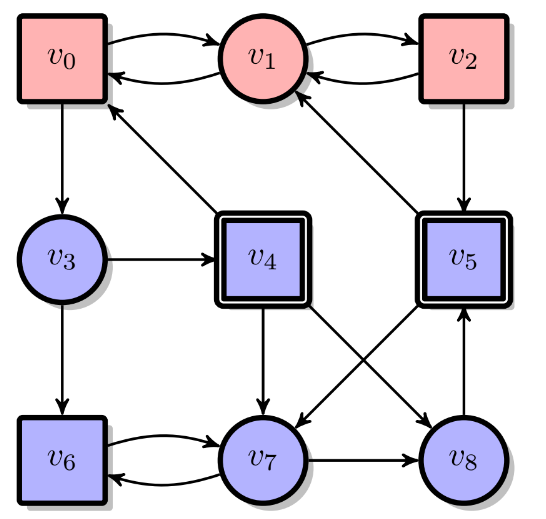
\includegraphics[width=0.4\linewidth]{figures/arena-example.png}
    \caption{\cite{infinite-games} Example of arena. The winning condition of player $0$ is to reach doubly-lined framed vertices (reachability game). Circular vertices are controlled by $P_0$, while rectangular ones are controlled by $P_1$. Blue and red vertices are $P_0$ and $P_1$ winning regions, respectively}
    \label{fig:enter-label}
\end{figure}

% \begin{lemma}
% For any game $\game$, it holds that $W_0(\game) \cap W_1(\game) = \emptyset$. In other words, the winning region of a player $i$ is the complement of the winning region for the player $1-i$, i.e. $W_i(\game) = V \setminus W_{1-i}(\game)$.
% \end{lemma}


\subsection{Safety and Reachability games}
The easiest games to solve, but at the same time enough interesting to analyze, are safety and reachability games.
Safety games consists in a game on an arena where we want to stay forever in a subset of vertices of the arena. In this case $P_0$ tries to stay forever in such subset, while $P_1$ tries to reach an outer vertex.
Reachability games consists in a game on an arena where we want to reach a subset of vertices of the arena. In this case $P_0$ tries to reach such subset, while $P_1$ tries to prevent $P_0$ to reach it by staying forever in the complement subset of vertices.

As maybe you could notice, safety and reachability games are dual: when $P_0$ is playing a safety game, $P_1$ is playing a reachability game, while when $P_0$ is playing a reachability game, $P_1$ is playing a safety game.

\begin{definition}[\cite{infinite-games} Occurrence set]
Given a play $\rho$, we denote as $Occ(\rho)$ the set of vertices occurring in $\rho$.
\end{definition}

\begin{definition}[\cite{infinite-games} Reachability game]
Let $\arena=\tuple{V, V_0, V_1, E}$ be an arena and let $R \subseteq V$ be a subset of $\arena$'s vertices. Then, the reachability condition $Reach(R)$ is defined as
\begin{flalign*}
    Reach(R) = \set{\rho \in V^\omega \; |\; Occ(\rho) \cap R \neq \emptyset}
\end{flalign*}
We call a game $\game = (\arena, Reach(R))$ a reachability game with reachability set $R$.
\end{definition}

\begin{definition}[\cite{infinite-games} Safety game]
Let $\arena = \tuple{V, V_0, V_1, E}$ be an arena and let $S \subseteq V$ be a subset of $\arena$'s vertices. Then, the safety condition $Safety(S)$ is defined as 
\begin{flalign*}
    Safety(S) = \set{\rho \in V^\omega \; | \; Occ(\rho) \subseteq S}
\end{flalign*}
We call a game $\game = (\arena, Safety(S))$ a safety game with safety set $S$.
\end{definition}

\begin{definition}[\cite{infinite-games} Dual Arena]
Let $\arena = \tuple{V,V_0,V_1,E}$ be an arena. The dual arena $\bar{\arena}$ of $\arena$ is defined as $\bar{\arena} = \tuple{V,V_1,V_0,E}$. 
\end{definition}

\begin{theorem}[\cite{infinite-games} Duality between safety and reachability games]
Let $\arena = \tuple{V,V_0,V_1,E}$ be an arena, let $\game = \tuple{A, SAFETY(S)}$ be a safety game with $S \subseteq V$ and define the reachability game $\game' = \tuple{\bar{\arena}, REACH(V \setminus S)}$. Then $W_i(\game) = W_{1-i}(\game')$ for each $i \in \set{0,1}$.
\end{theorem}

Let us now speak about algorithms to solve safety and reachability games. 
First of all, permit us to introduce some basic algorithms for solving such games on an explicit representation of the arena.
Afterwards, we will see that such algorithms can be empowered by BDD solving the games expressing the arena symbolically,

The fundamental algorithm to solve reachability is an algorithm based on fix-point computation of the 0-attractor. 
Basically, fixed a subset $R \subseteq V$ that we want to reach, we start computing the set of vertices from which the player $P_0$ can force to visit $R$ and $P_1$ can not avoid to visit $R$. Given such set of vertices we union with $R$ and do the same computation but now instead of reaching just $R$, we want to reach the new set resulting from the previous union. Going on like that we reach a point where the new computed set is not increasing anymore. 
That is the so-called fixed-point. 
We are sure to reach it because the set of vertices is finite.

\begin{definition}[\cite{infinite-games} i-Attractor]
Let $\game = (\arena, Reach(R))$ be a reachability game, where $\arena = \tuple{V, V_0, V_1, E}$ and $R \subseteq V$, and let $i \in \set{0,1}$ determine a player.
The controlled predecessor $CPre_i(R)$ of $R$ is defined as
\begin{flalign*}
CPre_i(R) = & \set{v \in V_i \; | \; \text{$v' \in R$ for some successor $v'$ of $v$}}\;\cup \\
            & \set{v \in V_{1-i} \; | \; \text{$v' \in R$ for all successors $v'$ of $v$}}
\end{flalign*}
The i-Attractor $Attr_i(R)$ in $\arena$ is defined by inductively applying the controlled predecessor via
\begin{flalign*}
& Attr_i^0(R) = R \\
& Attr_i^{n+1}(R) = Attr_i^n(R) \cup CPre_i(Attr_i^n(R)) \\
& Attr_i(R) = \bigcup_{n \in \Nat} Attr_i^n(R).
\end{flalign*}
Note that $Attractor_i^n \subseteq Attractor_i^{n+1}$ for all $n \geq 0$
\end{definition}

After having reached a fixed-point, we end up with a set of vertices which coincides with the winning region of $P_0$. 
Extracting a strategy from every nodes is easy. 
First save all controlled predecessors $CPre_0^0,\dots,CPre_0^n$, with $n \in \Nat$ such that $Attr_i^{n+1}(R) = Attr_i^{n}$ (we reached a fixed-point at attractor $n$) and $CPre_0^0 = R$. Then, we start from the last controlled predecessor $CPre_0^n$ and for each vertex $v \in CPre_0^n$ and $ v \in V_0$, we select an edge $\tuple{v,v'} \in E$ such that $v' \in CPre_0^{n-1}$. 
In other words, $P_0$ visits only those vertices from which $P_1$ can not avoid to get closer to the subset $R$, ending up in $CPre_0^9$ which is exactly the subset $R$. 
The strategy computation can be integrated in the algorithm in order to be more efficient.

Now that we are able to solve reachability game, we are able to solve safety game as well by exploiting duality. 
Indeed, as we have already seen, solving a safety game $\game = \tuple{\arena, SAFETY(S)}$ for $P_0$ is the same as solving a reachability game in the dual game $\bar{\game} = \tuple{\arena, REACH(V \setminus S)}$. 
Therefore, by applying the 1-attractor computation on $\game$, we can easily compute the winning region $W_0(\game)$ for $P_0$ by taking the complement of the winning region for $W_1(\game)$, that is $W_0(\game) = V \setminus W_1(\game)$.
Extracting a strategy for a safety game is easier.
Given a winning region $W_0(\game)$, for each vertex $v \in W_0(\game)$ and $v \in V_0$, we select an edge $\tuple{v,v'} \in E$ such that $v' \in W_0(\game)$. In other words, $P_0$ must visit only those vertices from which can be forced to stay in the winning region and so not escaping from $S$.

This algorithm based on fixed-point is very simple but also powerful because it allows to solve a reachability game, and therefore also safety games, in linear time. 

\begin{lemma}[\cite{infinite-games}]
Let $\game = (\arena, Reach(R))$ be a reachability game, where $\arena = \tuple{V, V_0, V_1, E}$ and $R \subseteq V$. Then, $W_0(\game) = Attr_0(R)$ and $W_1(\game) = V \setminus Attr_0(R)$.
\end{lemma}

\begin{lemma}[\cite{infinite-games}]
The attractor $Attr_i(R)$ in an arena $\arena$ with edges $E$ can be computed in linear time in $\card{E}$.
\end{lemma}


\subsection{Other types of games}
Besides safety and reachability games, there are many other types of games. 
In fact, safety and reachability games are the basis and are useful to synthesize safety formulas and co-safety formulas, respectively. 
Formulating more complex winning condition, we end up with different games useful for many reasons explored later.

% As we have already seen, there exist formulas which do not belong to neither of the two fragments. Such formulas require more sophisticated games, each of which is a generalization of some other games.  
So far we have studied games there the winner is determined by a prefix, but there are games where no prefix determines the winner: B{\"u}chi and co-B{\"u}chi games.
The winning condition for B{\"u}chi games is that some states in a set of states are visited infinitely many times.
The winning condition for co-B{\"u}chi games is that exactly all states visited infinitely many times are subset of a given set of states.

\begin{definition}[\cite{infinite-games} States visited infinitely many times]
Given a play $\rho$, we denote as $Inf(\rho)$ all states visited infinitely many times during the play.
\end{definition}

\begin{definition}[\cite{infinite-games} B{\"u}chi games]
Let $\arena = \tuple{V,V_0,V_1,E}$ be an arena and let $F \subseteq V$ be a subset of vertices. Then, the B{\"u}chi condition B{\"u}chi(F) is defined as
\begin{flalign*}
    \text{B{\"u}chi(F)} = \set{\rho \in V^\omega \; | \; Inf(\rho) \cap F \neq \emptyset}
\end{flalign*}
We call a game $\game = \tuple{\arena, \text{B{\"u}chi(F)}}$ a B{\"u}chi game.
\end{definition}

\begin{definition}[\cite{infinite-games} Co-B{\"u}chi games]
Let $\arena = \tuple{V,V_0,V_1,E}$ be an arena and let $F \subseteq V$ be a subset of vertices. Then, the co-B{\"u}chi condition coB{\"u}chi(F) is defined as
\begin{flalign*}
    \text{coB{\"u}chi(F)} = \set{\rho \in V^\omega \; | \; Inf(\rho) \subseteq F}
\end{flalign*}
We call a game $\game = \tuple{\arena, \text{coB{\"u}chi(F)}}$ a co-B{\"u}chi game.
\end{definition}

A generalization of the are previous games are \textit{Parity games}. 
In parity games the vertices of the arena are colored by natural number and the goal of player $0$ is to ensure that the minimal color seen infinitely often on a play is even. 
Equivalently, player $i$ wins if and only if the minimal color seen infinitely often has parity $i$. 
Thus, the color of a vertex denotes its importance (smaller colors are more important than larger ones) and its value for the players (vertices of even color are desirable for $P_0$, but undesirable for $P_1$ and vice-versa). 
B{\"u}chi and co-B{\"u}chi games can be expressed as parity games with two colors.

\begin{definition}[\cite{infinite-games} Parity games]
Let $\arena = \tuple{V,V_0,V_1,E}$ be an arena and let $\Omega \colon V \to \Nat$ be a coloring function of vertices. Then, the parity condition $Parity(\Omega)$ is defined as
\begin{flalign*}
    Parity(\Omega) = \set{\rho \in V^\omega \; | \; \max \set{Inf(\Omega(\rho_0)\Omega(\rho_1)\Omega(\rho_2)\dots)}\text{ is even}}
\end{flalign*}
We call a game $\game = \tuple{\arena, Parity(\Omega)}$ a parity game.
\end{definition}

All above games are determined with uniform positional winning strategies.

\subsection{Solving Safety and Reachability games symbolically}
In real applications is impossible to synthesize models from a $\ltl$ formula exploiting explicit representation of the arena. 
That is because the number of states of the arena is exponential in the number of state variables, ending up with too large games.
A solution to this problem is exploiting symbolic representations of regions states which can be much smaller than the represented state space. 
After a brief introduction to reactive synthesis through its game theory formulation, let us adapt the previous algorithms to work on symbolic representations.

In the first place, we need to represent the arena symbolically. 
That can be done by interpreting as Boolean variables the state variables and Boolean formulas the transition relation. 
We do not need two different types of arenas, because a safety arena is suitable both safety and reachability games according to what $P_0$ wants to solve. 
Therefore, for simplicity we define only arenas for safety games. 
Afterwards, we need to adapt the i-attractor computation. 
The only aspect we need to change is the controlled predecessor computation, which now is expressed in terms of $\exists$. $\forall$, $\land$, $\lor$ and Boolean formulas. 
Thanks to BDDs all previous operations are much easier to perform, enchanting the equivalence check of formulas and keeping a compact representation during these computations.

\begin{definition}[\cite{jacobs2015} Symbolic representation of games]
A symbolic representation for a safety game is given as tuple $\arena = \tuple{L,X_u,X_c,T(L,X_u,X_c,L'),Unsafe(L)}$ where: (i) $L$ is a set of Boolean state variables; (ii) $X_u$ is a set of Boolean uncontrollable inputs; (iii) $X_c$ is a set of Boolean controllable outputs; (iv) $T(L,X_u,X_c,L')$ is the transition relation, given as a quantifier-free Boolean formula over variables $L$, $X_u$, $X_c$ and $L'$, which represents the values of the state variables after the transition; (v) $Unsafe(L)$ is the region of unsafe states.
\end{definition}

Unlike before, we define $0$-attractor and $1$-attractor separately just because we explain the different order of quantification. 
We recall that Environment player plays first, so all arguments are made under this important assumption.

For safety games there are two algorithms that we may exploit to solve them. 
The first algorithm is defined as in the previous sub-section, that is computing the $1$-attractor and then obtaining the winning region for $P_0$ by taking the complement the attractor. 
In this case we state the controlled predecessor of a set of states $Unsafe(L)$ as the set of states $CPre_1^i(Unsafe(L))$ such that there exists a valuation of the uncontrollable inputs for which for all valuations of the controllable inputs, there exists a transition to some states in $CPre_1^{i-1}(Unsafe(L))$.
The second algorithm exploits the analogy with $\mu$-calculus model checking.
Indeed, since the computation of the winning region for both safety and reachability games laid on fix-point computation, we can see the winning region for  reachability game as the result of the Least Fixed Point (LFP) computation, and the winning region for a safety game as the result of the Greatest Fixed Point (GFP) computation.

For reachability games, the computation of $0$-attractor is a little different from the $1$-attractor one. Since the Environment player starts playing, the controlled predecessor of a set of states $Unsafe(L)$ is stated as the set of states $CPre_0^i(Unsafe(L))$ such that for each valuation of the uncontrollable inputs for which there exists a valuation of the controllable input, there exists a transition to some states in $CPre_0^{i-1}(Unsafe(L))$.

\begin{definition}[\cite{jacobs2015} Symbolic controlled predecessor for safety games]
Given arena $\arena$ and a set of states $S \subseteq L$, the controlled predecessor for $P_1$ (1-attractor) of $S$ is defined as
\begin{flalign*}
CPre_1(A) = \exists X_u \forall X_c \exists L'. A(L') \land T(L,X_u,X_c,L')
\end{flalign*}
\end{definition}

\begin{definition}[\cite{jacobs2015} Symbolic controlled predecessor for reachability games]
Given arena $\arena$ and a set of states $S \subseteq L$, the controlled predecessor for $P_0$ (0-attractor) of $S$ is defined as
\begin{flalign*}
CPre_0(A) = \forall X_u \exists X_c \exists L'. A(L') \land Trans(L,X_u,X_c,L')
\end{flalign*}
\end{definition}

Another key point of reactive synthesis is the strategy extraction from the winning region.
Symbolically, a strategy is a relation among Boolean formulas defining states, uncontrollable variables and controllable variables. 
For safety games, given a state in the winning region and an uncontrollable variable, we relate them with all possible controllable variables values such that in any case the next transition is still in the winning region. 
For reachability games, we look for a strategy which allows us to get us closer and closer to the unsafe states until we reach them. We provide a formal definition of non-deterministic strategy for reachability game in \autoref{sec:non-deterministic-strategy-reachability-game}, since we have found no information about it on other papers.
Whenever we have a non-determinstic strategy, no matter if it is generated from safety game or a reachability one, we want to determinize it in order to encode it in a circuit.
In principle, any determinization of the strategy can be chosen to obtain a function strategy for the system player, but there are many optimizations applicable to reduce the size of it. 
The one we have chosen is called co-factor method with care-set optimization.
Starting with the $\lambda$ non-deterministic strategy represented symbolically we apply the following steps for each $x_c \in X_c$ controllable variable:
\begin{enumerate}
    \item we restrict $\lambda$ to one output $x_c$, denote as $\lambda_{x_c}$;
    \item we compute positive ($p$) and negative (n) co-factors of $\lambda_{x_c}$, i.e. the values $s$ and $x_u$ for which $\lambda_{x_c}(s,x_u)$ can be $1$ or $0$, respectively;
    \item the combinatorial inputs that are neither in the positive nor in the negative co-factor are outsize of the winning region, representing situations that cannot occur. Thus, $\lambda(s,x_u)$ must be true in $p \land \neg n$ and false in $\neg p \land n$, which give us the set of care states, named care-set;
    \item we minimize the positive co-factor with the care-set to obtain the value of function $\lambda(s,x_u)$;
    \item we substitute variable $x_c$ in $\lambda$ by $\lambda(s,x_u)$ since other controllable outputs may be related to it;
    \item finally, we proceed with the next variable.
\end{enumerate}
% Regarding reachability games, we define the non-deterministic winning strategy $\lambda$ of a game $\game$ as the union of smaller strategies $\lambda_1,\dots,\lambda_n$ each of which consists in a strategy to go from a controlled predecessor to next one.
% Since we have not found any algorithm implementing such procedure exploiting BDDs, we have formulated one presented in \autoref{chapt:original-contributions}.

\begin{definition}[\cite{jacobs2015} Strategy for safety games]
Let $\game$ be a safety game represented symbolically and $W_0(\game)$ be the winning region of $P_0$ for the safety game. 
A non-deterministic winning strategy $\lambda \subseteq \Bool^L \times \Bool^{X_u} \times \Bool^{X_c}$ is defined as:
\begin{flalign*}
    \lambda(s,x_u) = \set{x_c \in \Bool^L \; | \; s \in W(L) \land \forall L' . T(s,x_u,x_c,L') \to W(L')}
\end{flalign*}
Analogously, $\lambda$ can be described as follows talking about set of states, set of uncontrollable variables and set of controllable variables:
\begin{flalign*}
    \lambda(L,X_u,X_c) = \exists L'. W_0(L) \land T(L,X_u,X_c,L') \land W_0(L')
\end{flalign*}
\end{definition}

% \begin{definition}[Strategy for reachability games]
% Let $\game$ be a reachability game on a safety arena represented symbolically and $CPre_0^0,\dots CPre_0^n$ be the set of controlled predecessors of $P_0$ computed solving reachability game. Recall that $CPre_0^0 = Unsafe(L)$.
% We define a set of non-deterministic winning strategies $\lambda_1,\dots,\lambda_n$ such that $\lambda_i \subseteq \Bool^L \times \Bool^{X_u} \times \Bool^{X_c}$ for each $i \in [1,n]$ and is defined as:
% \begin{flalign*}
%     \lambda_i(s,x_u) = \set{x_c \in \Bool^L \; | \; s \in Cpre_0^i \land \forall L' . (T(s,x_u,x_c,L')) \to CPre_0^{i-1}(L')}
% \end{flalign*}
% The whole non-deterministic winning strategy $\lambda \subseteq \Bool^L \times \Bool^{X_u} \times \Bool^{X_c}$ is defined as
% \begin{flalign*}
%     \lambda = \bigcup_{i=1}^n \lambda_i 
% \end{flalign*}
% \end{definition}

\begin{algorithm}[!htp]
\caption{\cite{BLOEM20073} Algorithm to determinize any non-deterministic strategy}
\label{alg:functional-strategy}
\begin{algorithmic}[1]
\Procedure{ExtractFunctionalStrategy}{$\arena$, $\lambda$}
    \State initialize $f$ as a map from controllable variable to strategy
    \For{$x_c \in X_c$}
        \State $\lambda_{x_c} \gets \exists X_c \setminus \set{x_c}.\; \lambda$
        \State $p \gets \lambda_{x_c}[1/x_c]$
        \State $n \gets \lambda_{x_c}[0/x_c]$
        \State $\text{\textit{care-set}} \gets (p \land \neg n) \lor (\neg p \land n)$
        \State $f[x_c] \gets \text{$p$ minimized w.r.t. \textit{care-set}}$
        \State $\lambda \gets \lambda[f[x_c]/x_c]$
    \EndFor
    \Return $f$
\EndProcedure
\end{algorithmic}
\end{algorithm}

\subsection{Linear Temporal Logic synthesis}
In previous sub-sections we introduced the game-theory notions needed to deal with Reactive Synthesis. Now we can see how to exploit those games to synthesis correct-by-construction models starting from a $\ltl$ formula. 
We will not go into details since the aim of the thesis is to deepen safety and co-safety fragments of $\ltl$, but it is still important to be aware about the relation between and games and $\ltl$ classes of formulas. 
Each game allows to synthesize a specific class of $\ltl$ formulas following the temporal hierarchy (\ref{fig:temporal-hierarchy}): safety and co-safety by safety and reachability games, obligation by weak-parity games, recurrence and persistence by reachability B{\"u}chi and co-B{\"u}chi games and reactivity by parity games.

We can formalize the synthesis of a generic $\ltl$ formula $\phi$ as a game. 
Such game is played on an arena $\arena$ labelled by a function $l$, such that each vertex of $\arena$ is associated to a set of atomic propositions. 
The winning condition is that the formula $\phi$ is satisfied on all labelled plays induced by a strategy.

\begin{definition}[LTL game]
Let $\arena=\tuple{V,V_0,V_1,E}$ be an arena, $\mathcal{P}$ be a set of propositions and $l \colon V \to 2^\mathcal{P}$ be labeling of vertices by atomic propositions. Then, the $\ltl$ condition $LTL(\phi,l)$ is defined as
\begin{flalign*}
    LTL(\phi,l) = \set{\rho \in V^\omega \; | \; (l(\rho_0)l(\rho_1)l(\rho_2)\dots,0) \models \phi}
\end{flalign*}
We call a game $\game=\tuple{\arena,LTL(\phi,l)}$ a LTL game. 
\end{definition}

Every LTL game can be solved by reducing it to parity game. 
First we obtain the corresponding NBA to $\phi$. 
Then, we construct the arena by converting the NBA to Deterministic Parity Automaton and finally we solve it. 
The overall procedure is $2EXPTIME$-complete.

Nevertheless, we investigate only safety and co-safety fragments and so we can study only safety and reachability games. 
In $\autoref{sec:ebr-ltl-synthesis}$ is presented a procedure to build safety arenas starting from $\ebrltl$ formulas.

\subsection{AIGER format in Reactive Synthesis}
AIGER format is highly used in reactive synthesis field. Indeed, it is common to represent safety arenas and synthesized controllers in extended AIGER format for reactive synthesis.
In safety Arenans each latch represents a state, both controllable and uncontrollable variables are inputs and the only output is the value of the synthesized formula.
The initial state of games is the conjunction of all latches, according to their initial value, i.e. if a latch $l_0$ initial value if false, then the conjunction is made with its negation $\neg l_0$, while if $l_0$ initial value is true, then the conjunction is made with itself with no changes.
The transition relation is a conjunction where a primed variable for each latch takes the same value as the input of itself.
The unsafe state is a conjunction of states we do not want to reach.

A synthesized controller is the safety arena on which was synthesized a strategy and it was modified encoding the strategy for controllable variables, which are no more inputs but becomes and gates and outputs. 


%!TEX root = ../../main.tex

\section{Reactive Synthesis from Extended Bounded Response LTL}
\label{sec:ebr-ltl-synthesis}

At this point we have reached the end of our journey. To sum up what we have explained so far, but also to see a practical use of them, let us have a look at the approach presented in \cite{geatti-2020-08} to reactive synthesis from $\ebrltl$ formulas. Note that we will give a brief indication of the whole procedure just to introduce the most important concepts. If you are interested in learning more about that, read the paper.

In \cite{geatti-2020-08} has been investigated a procedure to build the respective safety arena from any $\ebrltl$ formula.
In particular, the input of the procedure is a $\ebrltl$ formula, while the output is the Deterministic Symbolic Safety Automaton in extended AIGER format for reactive synthesis. In order to understand the whole procedure, we need to introduce some concepts: Safety Symbolic Automata, $Past\ebrltl$ and canonical $Past\ebrltl$.

In symbolic automata, states are identified by the value of state variables, and both initial and accepting states and the transition relation are represented as Boolean formulas. This allows them to be exponentially more succinct than equivalent explicitly represented automata. The transition relation $T(X,\Sigma,X')$ is built over states variables, input variables and a primed version of state variables representing the values of state variables st the next state.
A Symbolic Safety Automaton is a Safety Automaton where the states are represented symbolically.
For reactive synthesis, a crucial property of an automaton $\automaton$ is determinism, since in order to check if $\sigma \in \omegalang{(\automaton)}$ it suffices to check if the trace induced by $\sigma$ in $\automaton$ is accepting. For this reason we require that each SSA is deterministic.
Notice, this implies that for each $\sigma \in (2^\Sigma)^\omega$, there exists exactly one trace induced by $\sigma$ for any given Deterministic SSA. 

$Past\ebrltl$ is a logic equivalent to $\ebrltl$ which is easier to be converted in a corresponding canonical form (canonical $Past\ebrltl$) not containing nested occurrences of unbounded temporal operators, whose operands can be only full-past formulas and each of these is prefixed by an arbitrary number of next operators.

\begin{definition}[\cite{geatti-2020-08} Symbolic Safety Automata (SSA)]
A SSA is a tuple $\automaton = \tuple{V,I,T,S}$, where: (i) $V = X \cup \Sigma$ is a set of state variables and $\Sigma$ is a set of input variables; (ii) $I(X)$ is the set of initial states; (iii) $T(X,\Sigma,X')$ the transition relation; (iv) $S(X)$ the set of safe states.
\end{definition}

\begin{definition}[\cite{geatti-2020-08} Acceptance of SSA]
Let $\automaton$ be a SSA. 
A trace is a sequence $\tau  = \sequence{\tau_0,\tau_1,\dots} \in (2^V)^\omega$ of subsets $\tau_i$ of $V$ that satisfies the transition relation of $\automaton$, that is, such that for all $i \geq 0$, $T(X,\Sigma,X')$ is satisfied when $\tau_i$ is used to interpret variables from $X$ and $\Sigma$, and $\tau_{i+1}$ is used to interpret variables from $X'$. 
We say that a trace $\tau$ is induced by a word $\sigma = \sequence{\sigma_0,\sigma_1,\dots} \in (2^\Sigma)^\omega$ if and only if $\sigma_i = \tau_i \cap \Sigma$ for all $i \geq 0$.
A trace $\tau$ is accepting (or safe) if and only if $\tau_i$ satisfies $S(X)$ for all $i \geq 0$. 
The language of $\automaton$, denoted as $\lang{\automaton}$, is the set of all $\sigma \in (2^\Sigma)^\omega$ such that there exists an accepting trace induced by $\sigma$ in $\automaton$. 
\end{definition}

\begin{definition}[\cite{geatti-2020-08} Deterministic SSA]
A SSA $\automaton = \tuple{V,I,T,S}$ is deterministic if: (i) the formula $I$ has exactly one satisfying assignment; (ii) the transition relation is of the form $T(X,\Sigma,X') := \bigwedge_{x \in X} (x' \iff \beta_x(X \cup \Sigma))$, where each $\beta_x(X \cup \Sigma)$ is a Boolean formula over $X$ and $\Sigma$.
\end{definition}

\begin{definition}[\cite{geatti-2020-08} The logic $Past\ebrltl$] \label{def:past-ebrltl}
A $Past\ebrltl$ formula $\chi$ is inductively defined as follows:
\begin{flalign*}
&\psi    := p \; | \; \ltlNeg{\psi} \; | \; \ltlOr{\psi_1}{\psi_2} \; | \; \ltlY{\psi} \; | \; \ltlS{\psi_1}{\psi_2} \\
&\phi    := \psi \; | \; \ltlAnd{\phi_1}{\phi_2} \; | \; \ltlX{\phi} \; | \; \ltlG{\phi} \; | \; \ltlR{\ltlXexp{\psi}{i}}{\phi} \\
&\chi    := \lambda \; | \; \ltlOr{\chi_1}{\chi_2} \; | \; \ltlAnd{\chi_1}{\chi_2}
\end{flalign*}
\end{definition}

\begin{definition}[\cite{geatti-2020-08} Canonical $Past\ebrltl$] \label{def:canonical-past-ebrltl}
The \textit{canonical form} of $Past\ebrltl$ formulas is inductively defined as follows:
\begin{flalign*}
&\psi    := p \; | \; \ltlNeg{\psi} \; | \; \ltlOr{\psi_1}{\psi_2} \; | \; \ltlY{\psi} \; | \; \ltlS{\psi_1}{\psi_2} \\
&\phi    := \psi \; | \; \ltlG{\psi} \; | \; \ltlR{\psi_1}{\psi_2} \\
&\lambda := \phi \; | \; \ltlX{\lambda} \\
&\chi    := \lambda \; | \; \ltlOr{\chi_1}{\chi_2} \; | \; \ltlAnd{\chi_1}{\chi_2}
\end{flalign*}
\end{definition}

The transformation of $\ebrltl$ formulas into deterministic SSAs consists of three steps and the whole procedure is depicted in \autoref{fig:ebr-ltl-synthesis-procedure}:
\begin{itemize}
    \item a translation from $\ebrltl$ to $\pastebrltl$;
    \item a translation from $\pastebrltl$ to its canonical form;
    \item a transformation of canonical $\pastebrltl$ formulas into deterministic SSAs. 
\end{itemize}

\begin{figure}[!htp]
    \centering
    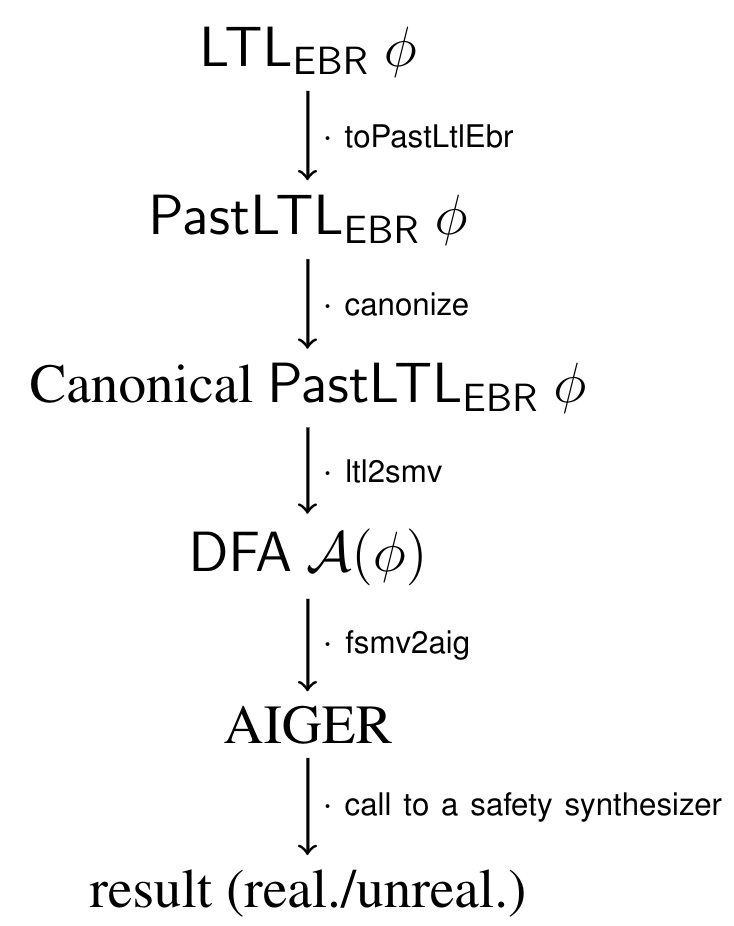
\includegraphics[width=0.4\linewidth]{figures/ebr-ltl-synthesis.png}
    \caption{\cite{geatti-2020-08} The overall procedure to synthesize a $\ebrltl$ formula}
    \label{fig:ebr-ltl-synthesis-procedure}
\end{figure}

The first step consists in translating each $\fpltl$ sub-formula in $\phi$ formula $\ebrltl$ into an equivalent one, which is of the form $\ltlXexp{\psi}{d}$, with $\psi \in \fpltl$ and $d \in \Nat$. This process is called pastification and is useful because full-past formulas can be represented by deterministic monitors, since "the past has already happened".

\begin{proposition}[\cite{geatti-2020-08} Soundness of pastification]
Let $\phi$ be a $\fbltl$ formula. For all state sequences $\sigma \in (2^\Sigma)^\omega$, all $i \in \Nat$ and all $d \geq D(\phi)$, it holds that
\begin{flalign*}
\sigma,i \models \phi \iff \sigma,i \models \ltlXexp{\Pi(\phi,d)}{d}
\end{flalign*}
\end{proposition}

The second step is the canonization of the $Past\ebrltl$ formula obtained from the previous step, in order to obtain an equivalent formula in canonical form. 
Canonical $Past\ebrltl$ formulas are Boolean combinations of formulas of the form $\ltlXexp{\psi_1}{i}$, $\ltlXexp{\ltlG{\psi_1}}{i}$, $\ltlXexp{\ltlR{\psi_1}{\psi_2}}{i}$, where $\psi_1$ and $\psi_2$ are full past formulas. 
Compared to general $Past\ebrltl$ formulas, formulas in canonical form do not admit neither nested unbounded operators nor next operators in front of the left-hand argument of a \textit{release}. The canonization of a $Past\ebrltl$ formula is obtained by applying a set of rewriting rules.
The particular shape of canonical $Past\ebrltl$ formulas makes it possible to encode the specifications into deterministic SSAs. The key observation is that $\fpltl$ formulas can be encoded into deterministic automata since these formulas exclusively talk about the past and so their truth can be evaluated at any single step depending only on previous steps, without making any guess about the future.

$Past\ebrltl$ in its canonical form combines full past formulas into a broader language that can still be turned into symbolic deterministic automata, exploiting the monitorability of universal temporal operators.
Consider the formula $\ltlG{\alpha}$. By observing a state sequence, at each step we can decide if a violation has occurred; indeed, if $\alpha$ is false at the current step, then the value of $\ltlG{\alpha}$ is certainly false for each of the previous steps. More generally, universal temporal formulas, such as $\ltlG{\alpha}$ and $\ltlR{\phi_1}{\phi_2}$, are monitorable, meaning that a violation of them can be decided on the basis of the observation of a finite number of steps. 
In particular, reporting an error in the next state can be done by considering only the current values. This means that any universal temporal operator can be monitored by adding a Boolean error variable with a deterministic transition relation. 
Therefore, despite not being able to evaluate the truth of a formula such as $\ltlG{\alpha}$, as it can be done in the case of past operators, we can nevertheless state in the accepting condition that an error state can never be reached. 
In this way, if the trace is accepting, that is an error state can never be reached, then we know that there are no violations, e.g., for $\ltlG{\alpha}$ we have forced $\alpha$ to be true in every state. 
Otherwise, if the trace is not accepting, that is an error state is reachable, we know that there is a (finite) violation and that the temporal formula was falsified at some step.
Therefore, we introduce an \textit{error bit} for each $\ltlXexp{\psi_1}{i}$, $\ltlXexp{\ltlG{\psi_1}}{i}$, $\ltlXexp{\ltlR{\psi_1}{\psi_2}}{i}$ of a canonical $Past\ebrltl$ formula.

Let $\phi$ be a canonical $Past\ebrltl$ formula over the alphabet $\Sigma = \C \cup \U$. We define the deterministic SSA $\automaton(\phi) = \tuple{V,I,T,S}$ as follows:
\begin{itemize}
    \item Variables. The set of state variables of the automaton is defined as $X = X_P \cup X_F \cup X_C$, where variables in $X_P$ track the truth value of all the full-past sub-formulas, variables in $X_F$ implement the monitoring mechanism and variables in $X_C$ are used to encode a binary counter used to monitor nested tomorrow operators. In particular, for $n$ nested tomorrow operators, a counter with $\log_2(n)$ bits is needed;
    \begin{flalign*}
        & X_P = \set{ \nu_\alpha \; | \; \text{$\alpha$ is a $\fpltl$ sub-formula of $\phi$}} \\
        & X_F = \set{error_\psi \; | \; \text{$\psi$ is a sub-formula of $\phi$ of the form $\ltlXexp{\psi}{i}$, $\ltlXexp{\ltlG{\psi}}{i}$ or $\ltlXexp{(\ltlR{\psi_1}{\psi_2})}{i}$}} \\
        & X_C = \set{counter_i \; | \; i \in \set{0,\dots,\log_2{d}} \text{with $d$ max. among all $X^d$ in $\phi$}}
    \end{flalign*}
    \item Initial state. All the state variables, including the counter bits, are initially false, that is $I(X) = \bigwedge_{x \in X} \ltlNeg{x}$;
    \item Transition relation. It is the conjunction of the transition functions of the binary counter and the monitors of each sub-formula of $\phi$.
    \item Safety condition. $S(X)$ is a Boolean formula obtained from $\phi$ by replacing each formula $\psi \in X_F$ by $\ltlNeg{error_\psi}$, i.e. $S(X) = \phi[\psi/\ltlNeg{error_\psi}]$.
\end{itemize}

We now define the monitors for the binary counter, used to handle nested \textit{tomorrow operators}, any formula $\psi \in \fpltl$ and any canonical $Past\ebrltl$. The monitor for the counter is defined as follows:
\begin{lstlisting}[language=smv, mathescape=true, caption=$\ebrltl$: counter]
next($counter_0$) := ($\bigwedge_{i=0}^n counter_i$) | $\neg counter_0$
next($counter_i$) := ($\bigwedge_{i=0}^n counter_i$) | (($counter_{i-1}$ | $counter_i$) & $\neg counter_i$)
\end{lstlisting}

If $\psi = \ltlS{\alpha}{\beta}$ or $\ltlY{\alpha}$, its monitor is defined as follows:
\begin{lstlisting}[language=smv,mathescape=true, caption=$\ebrltl$: yesterdat monitor]
next($\nu_{\ltlY{\alpha}}$) := $\nu_{\alpha}$
\end{lstlisting}
\begin{lstlisting}[language=smv,mathescape=true, caption=$\ebrltl$: since monitor]
DEFINE
    $\nu_{\ltlS{\alpha}{\beta}}$ := $\nu_\beta$ | ($\nu_\alpha$ & $\nu_{\ltlY{(\ltlS{\alpha}{\beta})}}$)
\end{lstlisting}

If $\psi$ is a propositional atom, a negation or a disjunction of full-past formulas, we define its monitor as follows:
\begin{lstlisting}[language=smv,mathescape=true, caption={$\ebrltl$: propositional atom, negation and disjunction monitors}]
DEFINE
    $\nu_p$ := $p$
    $\nu_{\ltlNeg{\alpha}}$ := !$\nu_\alpha$
    $\nu_{\ltlOr{\alpha}{\beta}}$ := $\nu_{\alpha}$ | $\nu_{\beta}$
\end{lstlisting}

For each formula $\phi$ of type $\ltlXexp{\psi}{i}$, where $\psi$ is a full-past formula, we introduce a new error bit $error_\phi$. Its monitor is defined as follows:
\begin{lstlisting}[language=smv,mathescape=true, caption=$\ebrltl$: next of proposition monitor]
next($error_{\ltlXexp{\psi}{i}}$) := case
    $error_{\ltlXexp{\psi}{i}}$ : TRUE;
    counter = i & !$\nu_{\psi}$ : TRUE;
    TRUE : FALSE;
  esac;
\end{lstlisting}

If $\phi = \ltlXexp{\ltlG{\psi}}{i}$, where $\psi$ is a full-past formula, we introduce a new error bit $error_\phi$ and define its monitor as follows:
\begin{lstlisting}[language=smv, mathescape=true, caption=$\ebrltl$: next of globally monitor]
next($error_{\ltlXexp{\ltlG{\psi}}{i}}$) := case
    counter < i : FALSE;
    !$error_{\ltlXexp{\ltlG{\psi}}{i}}$ & $\nu_{\psi}$ : FALSE;
    TRUE : TRUE;
  esac;
\end{lstlisting}

The same for $\phi = \ltlXexp{\ltlR{\psi_1}{\psi_2}}{i}$:
\begin{lstlisting}[language=smv, mathescape=true, caption=$\ebrltl$: next of release monitor]
next($error_{\ltlXexp{\ltlR{\psi_1}{\psi_2}}{i}}$) := case
    counter < i : FALSE;
    !$error_{\ltlXexp{\ltlR{\psi_1}{\psi_2}}{i}}$ & $\nu_{\psi_1^p}^i$ : FALSE;
    !$error_{\ltlXexp{\ltlR{\psi_1}{\psi_2}}{i}}$ & $\nu_{\psi_1}$ & $\nu_{\psi_2}$ : FALSE;
    !$error_{\ltlXexp{\ltlR{\psi_1}{\psi_2}}{i}}$ & $\nu_{\psi_2}$ : FALSE;
    TRUE : TRUE;
  esac;

next($\nu_{\psi_1^p}^i$) := case
    counter < i : FALSE;
    $\nu_{\psi_1^p}$ : TRUE;
    $\nu_{\psi_1^p}^i$ : TRUE;
    TRUE : FALSE;
  esac;
\end{lstlisting}

Moreover, we define two further monitors which are useful in the next chapter since, even though they are not defined in \cite{geatti-2020-08}.
The monitors are those for trigger and conjunction operators.
If $\phi = \ltlT{\alpha}{\beta}$ or $\phi = \ltlAnd{\alpha}{\beta}$, the monitors for such formulas can be defined as follows:
\begin{lstlisting}[language=smv, mathescape=true, caption=$\ebrltl$: trigger monitor]
DEFINE
    $\nu_{\ltlT{\alpha}{\beta}}$ := $\nu_\beta$ & ($\nu_\alpha$ | $\nu_{\ltlT{\alpha}{\beta}}$)
\end{lstlisting}
\begin{lstlisting}[language=smv, mathescape=true, caption=$\ebrltl$: conjunction monitor]
DEFINE
    $\nu_{\ltlAnd{\alpha}{\beta}}$ := $\nu_{\alpha}$ & $\nu_{\beta}$
\end{lstlisting}


\begin{figure}[!htp]
    \centering
    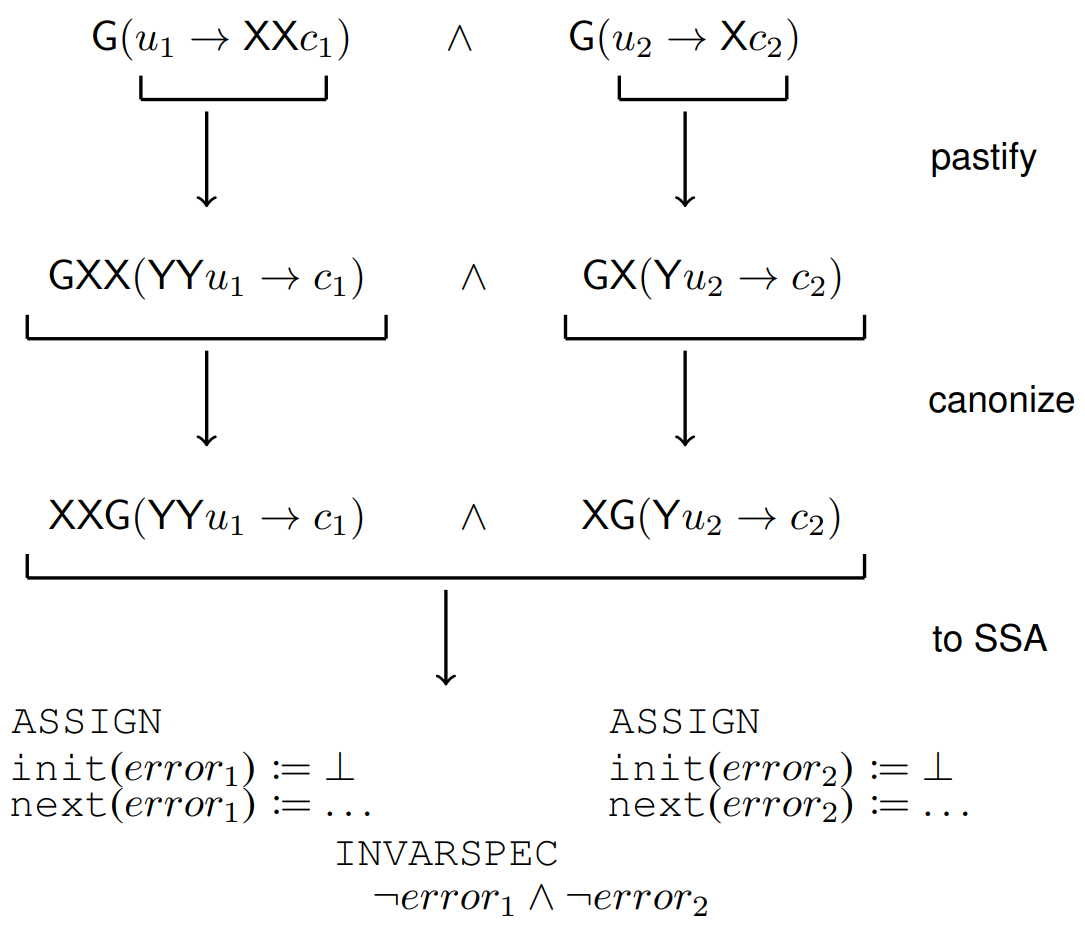
\includegraphics[width=0.6\linewidth]{figures/ebr-ltl-synthesis-example.png}
    \caption{\cite{geatti-2020-08} Example of $\ebrltl$ synthesis for the formula $\ltlAnd{\ltlG{(u_1 \to \ltlX{\ltlX{c_1}})}}{\ltlG{(u_2 \to \ltlX{c_2})}}$}
    \label{fig:ebr-ltl-synthesis-example}
\end{figure}

After having built the automaton, the respective safety game $\game = \tuple{\automaton_\phi, \C, \U}$ is converted to AIGER format and then given as input to the chosen safety synthesizer, completing the process described previously. It has been proved that the overall procedure belongs to $2EXPTIME$ complexity class, while it belongs to $EXPTIME$ if no constants are admitted managing to get rid of an exponential.

\begin{proposition}[\cite{geatti-2020-08} $\ebrltl$ synthesis complexity]
The realizability problem for $\ebrltl$ belongs to $2EXPTIME$. 
If no constant is admitted, it belongs to $EXPTIME$.
\end{proposition}

The $\ebrltl$ synthesis procedure is implemented in nuXmv under the command \lstinline{_ebr2fsmv}, which reads in input a $\ebrltl$ formula and produces the deterministic SSA of such formula. The SSA is represented by functional SMV modules, that is SMV modules characterized by only Boolean state variables and initial states and next transitions defined via \lstinline{init(var)} and \lstinline{next(var)} statements.
The conversion of SSAs from functional SMV to AIGER format is performed by the command \lstinline{fsmv2aig} implemeted in nuXmv.



%!TEX root = ../main.tex

\chapter{Original contributions} \label{chapt:original-contributions}

In this chapter we present all original contributions we made.

We formulate the problem to face, first textually and then formally. To do that we present four semantics for both safety and co-safety fragments: bounded-value, best-effort, bounded-steps and As Soon As Possible (ASAP).
Bounded-value semantics is the basis for best-effort one, while bounded-steps semantics for the ASAP one.
We prove that the ASAP semantics is just one of the possible instantiations of the best-effort semantics, showing that is possible to simulate the behaviour of ASAP semantics in the best-effort semantics.

The problem we want to deal with is an optimality test on a model, which we consider a closed-loop system for convenience.
In particular, given a plant, a controller and a safety or co-safety $\ltl$ formula, we want to figure out whether the closed-loop between plant and controller satisfies the formula and whether there exists another controller which does better than the given one according to some optimality principle. 
The optimality principle chosen by us is the one imposed by best-effort semantics because it is the most general one.
Then, we present a way to solve the problem by reduction to a reactive synthesis problem.

Finally, we provide a way to generate a non-deterministic strategy for reachability games.

%!TEX root = ../../main.tex

\section{Best-Effort semantics}
In this section we introduce the bounded-value and best-effort semantics.

The \textit{bounded-value semantics} is the first semantics presented because it is the basis for the other one.
Such semantics is useful to add a constraint to a value, ensuring that if a formula satisfies a state-sequence, then such value does not reach a constant value chosen a-priori. 
Note that we will not set the domain for the variable, but as long as the domain $\domain$ of the variable is a strict partially ordered set $\tuple{\domain,\prec}$ where $\prec$ is the strict partial order on $\domain$ (i.e. $\prec$ is irreflexive, antisymmetric, and transitive on $\domain$).
We define the bounded-value semantics for both safety and co-safety fragments.
The definitions in safety and co-safety fragments are different because, while for co-safety properties we need to look only all over the minimal prefix, for safety properties we need to look all over the trace which could be infinite.
The minimal prefix of a co-safety formula is a state-sequence prefix in which the formula holds the first time.
All prefixes containing the minimal prefix are sub-state-sequences satisfying the formula, but we do not mind what happens after the first time the formula has held.

\begin{definition}[Bounded-value semantics for co-safety formulas]
Let $\phi$ be a formula belonging to the co-safety fragment of $\ltl$, $\sigma$ be a state-sequence evaluated at position $i$, $\tuple{\domain,\prec}$ be a strict partially order set, $\sigma.v \in \domain$ a variable and $u \in \domain$ an upper bound to $\sigma.v$.
We say that $\phi$ is satisfied by $\sigma$ with upper-bound $u$ to $\sigma.v$ at position $i$, denoted as $\sigma,i \modelsBV{v \prec u} \phi$, if and only if
\begin{flalign*}
& \text{$\exists j \geq i$ such that $\sigma[i,j] \models \phi$, $\sigma[i,j-1] \not\models \phi$ and $\forall k \in [i,j].\; \sigma_k.v \prec u$}
\end{flalign*}
We say $\sigma \modelsBV{v \prec u} \phi$ if and only if $\sigma, 0 \modelsBV{v \prec u} \phi$.
\end{definition}

Differently from co-safety formulas where we can fix a point in time up to evaluate the formula, safety formulas are evaluated on possibly infinite state-sequences.
For this reason we define the bounded-value semantics for safety formulas inductively on the structure of safety formulas.
In order to avoid the formulation of bounded-value semantic for a negated generic formula, we consider only formulas in Negated Normal Form (NNF). 
The temporal operators needed to define safety formulas in NNF are: \textit{next}, \textit{yesterday}, \textit{release}, \textit{trigger} and \textit{since}.
Moreover, it is possible to define all temporal operators which are abbreviations of the ones listed here above that do not require negations in front of themselves, such as \textit{globally}, \textit{historically} and \textit{once}.
The basic idea is to check that the value of the chosen variable is related to the bound at every step.
The semantics is almost the same as the regular one, but we check the condition whenever we meet a proposition (negated or not) and whenever we take a step forward or backward.
In any other cases, the semantics does not change.
In fact, all abbreviations and equivalences holding in other safety dialects of $\ltl$, holds here too.

\begin{definition}[Bounded-value semantics for safety formulas]
Let $\phi$ be a formula belonging to the safety fragment of $\ltl$, $\sigma$ be a state-sequence evaluated at position $i$, $\tuple{\domain,\prec}$ be a strict partially order set, $\sigma.v \in \domain$ a variable and $u \in \domain$ an upper bound to $\sigma.v$.
We say that $\phi$ is satisfied by $\sigma$ with upper-bound $u$ to $\sigma.v$ at position $i$, denoted as $\sigma,i \modelsBV{v \prec u} \phi$, if and only if
\begin{flalign*}
&\sigma,i \modelsBV{v \prec u} p &\iff& & & p \in \sigma_i \land \sigma_i.v \prec u \\
&\sigma,i \modelsBV{v \prec u} \ltlNeg{p} &\iff& & & p \not\in \sigma_i \land \sigma_i.v \prec u \\
&\sigma,i \modelsBV{v \prec u} \ltlOr{\phi_1}{\phi_2} &\iff& & & \text{$\sigma,i \modelsBV{v \prec u} \phi_1$ or $\sigma,i \modelsBV{v \prec u} \phi_2$} \\
&\sigma,i \modelsBV{v \prec u} \ltlAnd{\phi_1}{\phi_2} &\iff& & & \text{$\sigma,i \modelsBV{v \prec u} \phi_1$ and $\sigma,i \modelsBV{v \prec u} \phi_2$} \\
&\sigma,i \modelsBV{v \prec u} \ltlX{\phi} &\iff& & & \sigma,i+1 \modelsBV{v \prec u} \phi \\
&\sigma,i \modelsBV{v \prec u} \ltlY{\phi} &\iff& & & \text{$i>0$ and $\sigma,i-1 \modelsBV{v \prec u} \phi$} \\
&\sigma,i \modelsBV{v \prec u} \ltlR{\phi_1}{\phi_2} &\iff& & & \text{either for all $j \geq i. \; \sigma,j \modelsBV{v \prec u} \phi_2$,} \\
& & & & & \text{or there exists $j \geq i$ such that $\sigma,j \modelsBV{v \prec u} \phi_1$ and} \\
& & & & & \text{$\sigma,w \modelsBV{v \prec u} \phi_2$ for all $i \leq w \leq j$} \\
&\sigma,i \modelsBV{v \prec u} \ltlS{\phi_1}{\phi_2} & \iff & & & \text{there exists $0 \leq j \leq i$ such that $\sigma,j \modelsBV{v \prec u} \phi_2$ and} \\
& & & & & \text{$\sigma,w \modelsBV{v \prec u} \phi_1$ for all $j < w \leq i$} \\
&\sigma,i \modelsBV{v \prec u} \ltlT{\phi_1}{\phi_2} & \iff & & & \text{either for all $0 \leq j \leq i. \; \sigma,j \modelsBV{v \prec u} \phi_2$,} \\
& & & & & \text{or there exists $j \in [0,i]$ such that $\sigma,j \modelsBV{v \prec u} \phi_1$ and} \\
& & & & & \text{$\sigma,w \modelsBV{v \prec u} \phi_2$ for all $j \leq w \leq i$}
\end{flalign*}
We say $\sigma \modelsBV{v \prec u} \phi$ if and only if $\sigma, 0 \modelsBV{v \prec u} \phi$.
\end{definition}

The bounded-value semantics is the basis of the best-effort semantics. 
The \textit{best-effort semantics} imposes to satisfy a formula with bounded-value semantics, where the bound is the least upper bound of values satisfying the formula with bounded-value semantics.
Therefore, there is no other value strictly smaller than the chosen one such that a state-sequence models a formula.
The best-effort semantics is useful because it imposes a constraint also to the upper bound.

\begin{definition}[Best-effort semantics]
Let $\phi$ be a formula belonging to either safety and co-safety fragment of $\ltl$, $\sigma$ be a state-sequence evaluated at position $i$, $\tuple{\domain,\prec}$ be a strict partially order set, $\sigma.v \in \domain$ a variable and $u \in \domain$ an upper bound to $\sigma.v$.
We say that $\phi$ is satisfied by $\sigma$ best-effort $u$ to $\sigma.v$ at position $i$, denoted as $\sigma, i \modelsBE{v \prec u} \phi$, if and only if
\begin{flalign*}
\sigma, i \modelsBV{v \prec u} \phi \land
\forall u' \prec u \; \sigma, i \not\modelsBV{v \prec u'} \phi
\end{flalign*}
We say $\sigma \modelsBV{v \prec u} \phi$ if and only if $\sigma, 0 \modelsBV{v \prec u} \phi$.
\end{definition}

\subsection{Notable examples}
In this sub-section we present two use-cases of bounded-value semantics and best-effort semantics. 
For these examples We consider the strict partially ordered set $\tuple{\Nat,<}$ and the corresponding relation $>$. Note that since the relation $<$ on the set of natural numbers has only one previous element for any number, to check whether a formula is satisfied best-effort with bound $u$, we just need to check whether is not satisfied with bound $u$ but not with bound $u-1$.

The first example regards a co-safety property. Suppose we are driving a car to reach a given position on a grid. In this case the plant is the car, while you, the driver, are the controller.
The car knows its internal position $(x,y)$ and has a battery level. 
At each step the battery decreases by $1$, starting from $100$. 
Whenever the battery level reaches $0$ the car cannot perform any further move.
Available moves are: up, down, left, right, right up, right down, left up and left down.
So we can move in all $8$ directions.

\begin{lstlisting}[language=smv, caption=Best-effort semantics: Car example (1)]
MODULE Car(move)
VAR
    x : 0..width;
    y : 0..length;
    battery : 0..max_battery;
DEFINE
    length := 20;
    width  := 20;
    starting_x := 0;
    starting_y := 0;
    max_battery := 100;
ASSIGN
    init(x) := starting_x;
    init(y) := starting_y;
    init(battery) := max_battery;
ASSIGN
    next(x) := case
        battery!=0 & (move=right | move=right_up | move=right_down) & x<width : x + 1;
        battery!=0 & (move=left | move=left_up | move=left_down) & x>0  : x - 1;
        TRUE : x;
    esac;
    next(y) := case
        battery!=0 & (move=up | move=left_up | move=right_up) & y<length : y + 1;
        battery!=0 & (move=down | move=left_down | move=right_down) & y>0  : y - 1;
        TRUE : y;battery!=0
    esac;
    next(battery) := case 
        move!=stop & battery > 0 : battery - 1;
        TRUE : battery;
    esac;
\end{lstlisting}

Let us define the first controller for the car: Driver1.
Driver1 accepts in input the position $(x,y)$ given by Car and aims to reach the position $(15,7)$ on the grid, but this driver does not know that it is possible to perform diagonal moves, so it goes only up, down, left and right.
The implemented strategy by Driver1 is to reach before the same x-axis as the goal one and the reach the same y-axis, ending up in the goal position.

\begin{lstlisting}[language=smv, caption=Best-effort semantics: Car example (2)]
MODULE Driver1(x,y)
VAR
    move : {up,down,right,left,
            right_up,right_down,
            left_up,left_down,
            stop};
DEFINE 
    goal_x := 15;
    goal_y := 7;
ASSIGN
    move := case
        x < goal_x  : right;
        x > goal_x  : left;
        y < goal_y  : up;
        y > goal_y  : down;
        TRUE : stop;
    esac;
\end{lstlisting}

Putting in closed-loop Car and Driver1, we can verify some properties on this system.
The easiest property is to verify whether Driver1 reaches the goal position, but keeping the value of the battery greater than $76$.
In bounded-value semantics, it would be something like that: 
\begin{flalign*}
    \closedloop{\text{C}}{\text{D}} \modelsBV{-\text{C.battery} < -76} \ltlF{(\ltlAnd{\text{C.x} = \text{D.goal\_x}}{\text{C.y} = \text{D.goal\_y}})}
\end{flalign*}

Note that since the bounded-value semantics is defined with a $<$ constraint, but we want to describe a $>$ constraint, it is enough multiply both terms by $-1$ in order to invert the inequality sign.
By running any the model checker NuSMV, we see that Driver1 reaches the goal position by always keeping the battery level greater than $76$.
We note that by lowering the bound $-76$ by $1$, so obtaining $-77$, the formula is no more satisfied, therefore we can say that such closed-loop satisfies best-effort the formula.

Now the question becomes, is Driver1 the optimal controller for Car?
To answer this question we need to show either another controller which satisfies the formula by keeping the battery level less than or equal to $-77$, or the not existence of such a controller.
In this case it is easy to see that a better controller is one which moves diagonally.
Driver2 is an example of controller moving also diagonally, which reaches the goal position by keeping the battery level $> 77$.
Therefore, Driver1 was not the optimal controller for that plant and that formula.

\begin{lstlisting}[language=smv, caption=Best-effort semantics: Car example (3)]
MODULE Driver2(x,y)
VAR
    move : {up,down,right,left,
            right_up,right_down,
            left_up,left_down,
            stop};
DEFINE 
    goal_x := 15;
    goal_y := 7;
ASSIGN
    move := case
        x < goal_x & y < goal_y  : right_up;
        x < goal_x & y > goal_y  : right_down;
        x < goal_x & y = goal_y  : right;
        x > goal_x & y < goal_y  : left_up;
        x > goal_x & y > goal_y  : left_down;
        x > goal_x & y = goal_y  : left;
        y < goal_y  & x = goal_x : up;
        y > goal_y  & x = goal_x : down;
        TRUE : stop;
    esac;
\end{lstlisting}

Regarding safety properties, we consider a water boiler with a controller which must keep the water temperature between $30$ and $70$ degrees.
The boiler, when it is on increments the temperature by $1$, while when it is off the water temperature drops one degree at a time.
We also consider the energy consumption to warm the water, which is exactly the number of steps in which the boiler is on.
Whenever the controller turns off the boiler, the energy consumption is set to $0$.

\begin{lstlisting}[language=smv, caption=Best-effort semantics: Boiler example (1)]
MODULE Boiler(on)
VAR 
    temp  : 0..100;
    energy : 0..100;
ASSIGN
    init(temp) := 50;
    next(temp) := case
        temp=100 : 100;
        temp=0 : 0;
        on  : temp + 1;
        !on : temp - 1;
    esac;
    init(energy) := 0;
    next(energy) := case
        !on : 0;
        on & energy < 100 : energy + 1;
        TRUE : energy;
    esac;
\end{lstlisting}

We define Controller1 in such a way that turns on the boiler exactly when the water temperature goes lower than $40$ degrees and turns off the boiler when the water temperature reaches $50$ degrees.

\begin{lstlisting}[language=smv, caption=Best-effort semantics: Boiler example (2)]
MODULE Controller1(temp)
VAR
    on : boolean;
ASSIGN
    init(on) := FALSE;
    next(on) := case
        temp <= 40 : TRUE;
        temp >= 50 : FALSE;
        TRUE : on;
    esac;
\end{lstlisting}

We can verify some properties on the closed-loop, like verifying that the water temperature is always between the required range and we use little energy as possible.

\begin{flalign*}
    \closedloop{\text{B}}{\text{C}} \modelsBV{\text{B.energy} < 13} \ltlG{(\ltlAnd{\text{B.temp} \geq 30}{\text{B.temp} \leq 70})}
\end{flalign*}

It is easy to see that the formula we are verifying is also satisfied best-effort by Controller1 with upper-bound $13$.
Unfortunately, Controller1 is not optimal because there exists other controller which are satisfied with a lower upper-bound. 
One among them is Controller2 which satisfies the formula keeping the energy always lower than $6$.

\begin{lstlisting}[language=smv, caption=Best-effort semantics: Boiler example (3)]
MODULE Controller2(temp)
VAR
    on : boolean;
ASSIGN
    init(on) := FALSE;
    next(on) := case
        temp < 40 : TRUE;
        temp > 41 : FALSE;
        TRUE : on;
    esac;
\end{lstlisting}

%!TEX root = ../../main.tex

\section{As Soon As Possible (ASAP) semantics}
In this section we introduce another semantics which captures the behaviour of systems that must response promptly.
This semantics is called As Soon As Possible (ASAP) semantics and forces a formula to satisfy a state-sequence in as few steps as possible.
To define the ASAP semantics we exploit another semantics, called \textit{bounded-steps semantics}, which forces a formula to be satisfied in a certain bound of time.
Similarly to the bounded-value semantics, we define the bounded-steps semantics for both co-safety and safety fragments of $\ltl$. 

In the co-safety fragment we say that a formula is satisfied by a state-sequence at position $i$ with maximum number of steps $u$, if such formula is satisfied in the prefix from $i$ to $u+i$.

\begin{definition}[Co-safety LTL bounded-steps semantics]
Let $\phi$ be a formula belonging to the co-safety fragment, $\sigma$ a state-sequence evaluated at position $i$ and $u \in \Nat$ maximum number of steps.
We say that $\sigma$ satisfies $\phi$ at position $i$ in $u$ steps, denoted as $\sigma,i \modelsUB{u}{} \phi$, if and only if
\begin{flalign*}
    \sigma[i,u+i] \models \phi
\end{flalign*}
We say that $\sigma \modelsUB{u}{} \phi$ if and only if $\sigma,0 \modelsUB{u}{} \phi$.
\end{definition}

In the safety fragment the definition is a little bit different.
First of all, we name the number of steps already performed as depth.
The difference between the upper bound and the depth gives us the number of steps that we are still allowed to do.
We need to understand what means for a state-sequence satisfying a formula in $u$ steps.
Here there are two possible interpretations: either defining such semantics similar to the semantics induced by the full-bounded dialect of $\ltl$ ($\fbltl$), therefore evaluating a property over a prefix from $i$ to $u+i$ like in the co-safety case, or evaluating over a finite prefix only formulas which are both in co-safety and safety.
In the first case we would define the semantics of formulas such as $\ltlGbounded{\phi}{[d,u]}$, $\ltlFbounded{\phi}{[d,u]}$ and $\ltlUbounded{\phi_1}{\phi_2}{[d,u]}$, but as we have already said, it is the same semantics induced by the full-bounded dialect of $\ltl$. 
Instead, we have preferred to investigate the latter case, where the semantics evaluates only both safety co-safety formulas over a prefix from $d$ to $u$. 
Analogously to the bounded-value semantics, the bounded-steps semantics is defined inductively on the structure of the formula to evaluate.
Basic cases are \textit{boolean propositions}, \textit{negation} of a boolean proposition, \textit{or} and \textit{and} operators, while more interesting cases are the \textit{next} and \textit{yesterday} temporal operators.

\begin{definition}[Safety LTL bounded-steps semantics]
Let $\phi$ be a formula belonging to the safety fragment, $\sigma$ a state-sequence evaluated at position $i$, $u \in \Nat$ maximum number of steps and $d \in \Nat$ be the depth such that $d \leq u$.
We say that $\sigma$ satisfies $\phi$ at position $i$ in $u$ steps with depth $d$, denoted as $\sigma,i \modelsUB{u}{d} \phi$, if and only if
\begin{flalign*}
&\sigma,i \modelsUB{u}{d} p &\iff& & & p \in \sigma_i \land 0 \leq d \leq u \\
&\sigma,i \modelsUB{u}{d} \ltlNeg{p} &\iff& & & p \not\in \sigma_i \land 0 \leq d \leq u \\
&\sigma,i \modelsUB{u}{d} \ltlOr{\phi_1}{\phi_2} &\iff& & & \text{$\sigma,i \modelsUB{u}{d} \phi_1$ or $\sigma,i \modelsUB{u}{d} \phi_2$} \\
&\sigma,i \modelsUB{u}{d} \ltlAnd{\phi_1}{\phi_2} &\iff& & & \text{$\sigma,i \modelsUB{u}{d} \phi_1$ and $\sigma,i \modelsUB{u}{d} \phi_2$} \\
&\sigma,i \modelsUB{u}{d} \ltlX{\phi} &\iff& & & \sigma,i+1 \modelsUB{u}{d+1} \phi \\
&\sigma,i \modelsUB{u}{d} \ltlY{\phi} &\iff& & & \text{$i>0$ and $\sigma,i-1 \modelsUB{u}{d-1} \phi$} \\
&\sigma,i \modelsUB{u}{d} \ltlR{\phi_1}{\phi_2} &\iff& & & \text{either for all $j \geq i. \; \sigma,j \modelsUB{u}{d} \phi_2$,} \\
& & & & & \text{or there exists $j \geq i$ such that $\sigma,j \modelsUB{u}{d} \phi_1$ and} \\
& & & & & \text{$\sigma,w \modelsUB{u}{d} \phi_2$ for all $i \leq w \leq j$} \\
&\sigma,i \modelsUB{u}{d} \ltlS{\phi_1}{\phi_2} & \iff & & & \text{there exists $0 \leq j \leq i$ such that $\sigma,j \modelsUB{u}{d} \phi_2$ and} \\
& & & & & \text{$\sigma,w \modelsUB{u}{d} \phi_1$ for all $j < w \leq i$} \\
&\sigma,i \modelsUB{u}{d} \ltlT{\phi_1}{\phi_2} & \iff & & & \text{either for all $0 \leq j \leq i. \; \sigma,j \modelsUB{u}{d} \phi_2$,} \\
& & & & & \text{or there exists $j \in [0,i]$ such that $\sigma,j \modelsUB{u}{d} \phi_1$ and} \\
& & & & & \text{$\sigma,w \modelsUB{u}{d} \phi_2$ for all $j \leq w \leq i$}
\end{flalign*}
We say that $\sigma,i \modelsUB{u}{} \phi$ if and only if $\sigma,i \modelsUB{u}{0} \phi$, while $\sigma \modelsUB{u}{} \phi$ if and only if $\sigma, 0 \modelsUB{u}{} \phi$.
\end{definition}

After having defined the bounded-steps semantics, we can finally present the \textit{ASAP semantics}, thanks to which we capture the fact to satisfy a formula in as few number of steps as possible.
The ASAP semantics is defined exploiting bounded-steps semantics and we require that the upper bound is as tight as possible, therefore it is the least upper bound of the bounds satisfying bounded-steps a formula.

\begin{definition}[ASAP semantics]
Let $\phi$ be a formula belonging to either the safety or co-safety fragment, $\sigma$ a state-sequence at position $i$ and $u \in \Nat$ maximum number of steps.
We say that $\sigma$ satisfies $\phi$ at position $i$ as soon as possible in $u$ steps, denoted as $\sigma, i \modelsASAP{u}{} \phi$, if and only if
\begin{flalign*}
    \sigma, i \modelsUB{u}{} \phi \land 
    \sigma, i \not\modelsUB{u-1}{} \phi
\end{flalign*}
We say that $\sigma \modelsASAP{u}{} \phi$ if and only if $\sigma, 0 \modelsASAP{u}{} \phi$.
\end{definition}

%!TEX root = ../../main.tex

\subsection{Notable examples}
% Esempi notevoli che mostrino l'utilità e le potenzialità della semantics best-effort e ASAP. 

In this sub-section we give some notable use-cases of bounded-value semantics and ASAP semantics using $\ebrltl$ to express properties.

The first example is a typical bounded response requirement, where whenever a request ($r$) is issued, the controller has to answer a grant ($g$) at most $5$ time units after the request.
\begin{flalign*}
    \phi_1 \equiv \ltlG{(\ltlImpl{r}{\ltlFbounded{g}{[0,5]}})}
\end{flalign*}

In $\phi_1$ there is already a bound on the maximum number of steps of $g$, but with our semantics we could be even tighter without changing the formula syntax, such as forcing the grant to be issued immediately or in 2 steps.

\begin{flalign*}
\closedloop{P}{C} \modelsUB{0}{} \ltlG{(\ltlImpl{r}{\ltlFbounded{g}{[0,5]}})} \\
\closedloop{P}{C} \modelsUB{2}{} \ltlG{(\ltlImpl{r}{\ltlFbounded{g}{[0,5]}})}
\end{flalign*}

Some other examples could be the ones presented for the best-effort semantics.
Considering the car presented in the previous section, we could force it to reach the goal in some bound of steps.

\begin{flalign*}
    \closedloop{\text{M}}{\text{D}} \modelsUB{13}{} \ltlF{(\ltlAnd{\text{M.x} = \text{D.goal\_x}}{\text{M.y} = \text{D.goal\_y}})}
\end{flalign*}

%!TEX root = ../../main.tex

\subsection{Relation between best-effort and ASAP semantics} \label{subsec:relation-best-effort-asap}
During the definition of ASAP semantics, you could have noticed that there exists a relation with the best-effort semantics using as strict partially ordered set $\tuple{\Nat,<}$.
Indeed, ASAP semantics can be formulated through best-effort semantics and in this section we prove it. As usual, we split the proof according to the type of formulas, so a proof for co-safety fragment and another one for safety fragment.
The idea behind the two proofs is the same, that is adding a variable to the plant which simulates the behaviour of the ASAP semantics.
Note that for convenience and clarity, we define the behaviour of those variables by SMV language.

Regarding the co-safety fragment of $\ltl$, that is for sure the easiest case because we evaluate formulas on prefixes of state-sequences.
Moreover, both best-effort and ASAP semantics are not defined inductively but through their behaviour on a finite prefix of a state-sequence.
In this case we add a variable named steps which is incremented by $1$ at every step and bound on such variable. 
In this way we can keep up with the steps taken and see whenever we exceed the maximum number of steps without the formula being true.

\begin{theorem}[Best-effort and ASAP equivalence for co-safety formulas]
\label{thm:asap-best-effort-co-safety}
Let $\closedloop{\plant}{\controller}$ be a closed-loop model of a system with plant and controller, $\sigma$ be any trace of such model evaluated at position $i$, $\phi$ a formula belonging to co-safety fragment of $\ltl$ and $u \in \Nat$ be a constant number.
We show that, by adding the variable $\plant.steps$ to the plant, the following statement holds
\begin{flalign*}
   \sigma, i \modelsBE{steps < u+i+1} \phi \iff
   \sigma, i \modelsASAP{u+i}{} \phi
\end{flalign*}

\begin{proof}
First of all we define the behaviour of the new state variable $steps$ in the following way: initially $steps$ has value $i$ and at each step it is increased by $1$.
\begin{lstlisting}[language=smv,mathescape=true]
ASSIGN
    init(steps) := i;
    next(steps) := steps + 1;
\end{lstlisting}

\begin{itemize}
\item ($\sigma, i \modelsBE{steps < u+i+1} \phi \implies \sigma, i \modelsASAP{u+i}{} \phi$)

By hypothesis we know that (1) $\sigma,i \modelsBV{steps < u+i+1} \phi$ and (2) $\sigma,i \not\modelsBV{steps < u+i} \phi$.
By definition of bounded-value semantics we know that $\exists j \geq i$ such that $\sigma[i,j] \models \sigma$, $\sigma[i,j-1] \not\models \sigma$ and $\forall k \in [i,j].\; \sigma_k.steps < u+i+1$.
Since the variable $\sigma.steps$ keeps up with the number of steps performed by the model, it is easy to see that, when $\sigma,i \modelsBE{steps < u+i+1} \phi$, has been performed exactly $u+i$ steps and therefore is equivalent to $\sigma[i,u+i] \models \phi$.
More formally: (3) such $j$ exists and it is $j=u+i$, (4) $\sigma[i,u+i] \models \sigma$, (5) $\sigma[i,u+i-1] \not\models \phi$ and $\forall k \in [i,u+i].\; \sigma_k.steps < u+i-1$.

By (4) and (5) and definition of ASAP semantics, we claim $\sigma,i \modelsASAP{u+i}{} \phi$

\item ($\sigma,i \modelsASAP{u+i}{} \phi \implies \sigma,i \modelsBE{steps < u+i+1} \phi$)

By hypothesis we know that $\sigma,i \modelsUB{u+i}{} \phi$ and $\sigma,i \not\modelsUB{u+i-1}{} \phi$, from which we derive (1) $\sigma[i,u+i] \models \phi$ and (2) $\sigma[i,u+i-1] \not\models \phi$, by definition of bounded-steps semantics.
We note that the variable $\sigma.steps$ keeps up with the number of steps performed by the models.
For this reason it is easy to see that (3) $\forall k \in [i,u+i].\; \sigma_k.steps < u+i+1$, since $steps$ at position $\sigma_k$ has exactly value $k$.
By (1), (2), (3) and definition of bounded-value semantics, we derive (4) $\sigma,i \modelsBV{steps < u+i+1} \phi$.
We note that in (2) the statement is falsified just because $\phi$ is falsified in the prefix, i.e. when $steps$ is always less than or equal to $u+i$, concluding (5) $\sigma,i \not\modelsBV{steps < u+i} \phi$.

Therefore, by (4), (5) and definition of best-effort semantics, we claim $\sigma,i \modelsBE{steps < u+i+1} \phi$. 
\end{itemize}
\end{proof}
\end{theorem}

As we told previously, the safety case is the hardest one but also the most interesting between the two cases.
Here we cannot simply set some counters and force them to count the number of steps already performed, because the semantics is defined inductively on the structure of $\phi$.
Therefore, the variables system which allows us to simulate the behaviour of the ASAP semantics is more complex.
The underlying idea is to add to the plant the deterministic monitor of $\phi$, explained in \autoref{sec:ebr-ltl-synthesis}, to monitor which sub-formulas are true at each step. 
Then we associate at each sub-formula a cost which corresponds to minimum number of next minus number of yesterday in such sub-formula required to make it true.
Therefore, the formula $\phi$ has a cost which depends on the formula itself and by the costs of sub-formulas which are true.
The cost of a formula is the dual of the concept of depth. 
Indeed, the depth in ASAP semantics for safety formulas reaches its maximum value when it reaches the propositional case, where we check whether we went over the maximum number of steps or not, and the minimum value at the beginning with $\phi$. On the contrary, the cost of a formula reaches the maximum value at the beginning with $\phi$ and its minimum value when it reaches the propositional case.
In the latter case we perform the check the bound on the cost of $\phi$.

\begin{theorem}[Best-effort and ASAP equivalence for safety formulas]
\label{thm:asap-best-effort-safety}
Let $\closedloop{\plant}{\controller}$ be a closed-loop model of a system with plant and controller, $\sigma$ be any trace of such model evaluated at position $i$, $\phi$ a formula belonging to the safety fragment of $\ltl$ and $u \in \Nat$ be a constant number.
We show that by adding the variable $\plant.cost_\phi$ to the plant, the following statement holds 
\begin{flalign*}
   \sigma,i \modelsBE{cost_\phi < u+1} \phi \iff 
   \sigma,i \modelsASAP{u}{u-cost_\phi} \phi
\end{flalign*}

\begin{proof}
From \cite{geatti-2021-09} we know that there exists a formula $\phi' \in \pastebrltl$ such that $\phi \equiv \phi'$ for any safety formula $\phi$.
From the work made in \cite{geatti-2020-08} we know that it is possible to create a Deterministic Safety Automaton $\automaton$ such that $\omegalang{(\automaton)} \equiv \omegalang{(\phi')}$. 
In such automaton we have a state variable for each sub-formula of the type $\ltlXexp{\psi_1}{i}$, $\ltlXexp{\ltlG{\psi_1}}{i}$ and $\ltlXexp{(\ltlR{\psi_1}{\psi_2})}{i}$, where $\psi_1,\psi_2 \in \fpltl$. Such state variables check the falsity of those sub-formulas, therefore one of them becomes true whenever the monitoring sub-formula is false.
Moreover, we have a state variable for each full-past sub-formula checking the truthfulness of a sub-formula, therefore one of them becomes true whenever the monitoring sub-formula is true.

At this point, we define a state variable corresponding to the cost of a sub-formula monitored by other state variables.
The state variables that we add are: 
\begin{itemize}
    \item $C_P$: the set of state-variables with the cost of a full past sub-formula (full-past layer of $Canonical Past\ebrltl$);
    \item $C_E$: the set of state-variables with the cost of sub-formulas of the form $\ltlXexp{\psi_1}{i}$, $\ltlXexp{\ltlG{\psi_1}}{i}$ and $\ltlXexp{(\ltlR{\psi_1}{\psi_2})}{i}$, monitored by error variables (future layer of $Canonical Past\ebrltl$);
    \item $C_F$: the set of variables with the cost of sub-formulas which are combinations between themselves and error variables (Boolean layer of $Canonical Past\ebrltl$).
    \begin{flalign*}
    & C_P = \set{ cost_{\nu_\alpha} \; | \; \text{$\alpha$ is a $\fpltl$ sub-formula of $\phi$}} \\
    & C_E = \set{ cost_{error_\psi} \; | \; \text{$\psi$ is a sub-formula of $\phi$ of the form $\ltlXexp{\psi_1}{i}$, $\ltlXexp{\ltlG{\psi_1}}{i}$ and $\ltlXexp{(\ltlR{\psi_1}{\psi_2})}{i}$}} \\
    & C_F = \set{ cost_\chi \; | \; \text{$\psi$ is a sub-formula of $\phi$ of the form $\chi_1 \lor \chi_2$ and $\chi_1 \land \chi_2$}}
    \end{flalign*}
\end{itemize}

Then we add a further state-variable named $cost_\phi$ which is the maximum cost of $\phi$ at each step. The cost of a formula is defined as follows:
\begin{itemize}
    \item \textit{Boolean proposition}: if the formula is a Boolean proposition (positive or negative), its cost is $0$.
    \item or: if the formula is the logical or between two sub-formulas, then we take the minimum cost between the sub-formulas which are true;
    \item \textit{and}: if the formula is the logical and between two sub-formulas, then we take the maximum cost between them;
    \item \textit{next}: if the formula is the next of a sub-formula, we increment by $1$ the cost of such sub-formula;
    \item \textit{yesterday}: if the formula is the yesterday of a sub-formula, we decrement by $1$ the cost of such sub-formula;
    \item \textit{release}: if the formula is the trigger between two sub-formulas, we take he maximum cost between the sub-formulas which are true;
    \item \textit{trigger}: if the formula is the trigger between two sub-formulas, we take he maximum cost between the sub-formulas which are true;
    \item \textit{since}: if the formula is the trigger between two sub-formulas, we take he maximum cost between the sub-formulas;
\end{itemize}

Note that in all cases we consider only sub-formulas which are true, since if a sub-formula is false we can ignore its cost.

For sure we need to adapt this concept to our monitor and the result can be seen here below. 
For each cost variable we assign the cost as described previously only if the formula corresponding to that cost is true, otherwise the cost is a value that for sure exceed the bound, that is $u$.

\begin{lstlisting}[language=smv, mathescape=true]
DEFINE
    -- Pure past layer
    $cost_p$ := 0
    $cost_{\ltlNeg{p}}$ := 0
    $cost_{\ltlOr{\alpha_1}{\alpha_2}}$ := case
        $\nu_{\ltlOr{\alpha_1}{\alpha_2}}$ : $\min_{\alpha \in \set{\alpha_1,\alpha_2}}$ {$cost_{\alpha}$ | $\nu_{\alpha}$ is true}
        TRUE : u;
    esac;
    $cost_{\ltlAnd{\alpha_1}{\alpha_2}}$ := case
        $\nu_{\ltlAnd{\alpha_1}{\alpha}}$ : max{$cost_{\alpha_1}$,$cost_{\alpha_2}$}
        TRUE : u;
    esac;
    $cost_{\ltlT{\alpha_1}{\alpha_2}}$ := case
        $\nu_{\ltlT{\alpha_1}{\alpha_2}}$ : $\max_{\alpha \in \set{\alpha_1,\alpha_2}}$ {$cost_{\alpha}$ | $\nu_{\alpha}$ is true}
        TRUE : u;
    esac;
    $cost_{\ltlY{\alpha}}$ := $cost_{\alpha}$ - 1
    $cost_{\ltlS{\alpha_1}{\alpha_2}}$ := case
        ($\nu_{\ltlS{\alpha_1}{\alpha_2}}$) : case $\nu_{\alpha_2}$ : $cost_{\alpha_2}$; $!\nu_{\alpha_2}$ : max{$cost_{\alpha_1}$,$cost_{\alpha_2}$};
        TRUE : u;
    esac;
    -- Future layer
    $cost_{\ltlXexp{\alpha}{i}}$ := $cost_\alpha$ + i
    $cost_{\ltlXexp{(\ltlR{\alpha_1}{\alpha_2})}{i}}$ := case
        $\neg error_{\ltlXexp{(\ltlR{\alpha_1}{\alpha_2})}{i}}$ & $\neg \nu^i_{\alpha_1^p}$ : $\max_{\alpha \in \set{\alpha_1,\alpha_2}}$ {$cost_{\alpha}$ | $nu_{\alpha}$ is true} + i
        TRUE: u;
    esac;
    -- Boolean layer
    $cost_{\ltlOr{\chi_1}{\chi_2}}$ := case
        $\chi_1$ | $\chi_2$ : $\min_{\chi \in \set{\chi_1,\chi_2}}$ {$cost_{\chi}$ | $\nu_{\chi}$ is true};
        TRUE: u;
    esac;
    $cost_{\ltlAnd{\chi_1}{\chi_2}}$ := case
        $\chi_1$ & $\chi_2$ : max{$cost_{\chi_1}$, $cost_{\chi_2}$};
        TRUE: u;
    esac;
\end{lstlisting}

\noindent ($\sigma,i \modelsBE{cost_\phi < u+1} \phi \implies \sigma,i \modelsASAP{u}{u-cost_\phi} \phi$) \\
\noindent We prove the statement by structural induction over $\phi$.

\noindent (Base case)
\begin{itemize}
    \item ($\phi = p$) \\
    Let $\phi$ be a formula of the shape $\phi = p$. 
    By definition of cost of $\phi$, $cost_\phi = 0$.
    By hypothesis we know that $\sigma,i \modelsBE{0 < u+1} \phi$, i.e. (1) $\sigma,i \modelsBV{0 < u+1} \phi$ and (2) $\sigma,i \not\modelsBV{0 < u} \phi$ with $u \geq 0$. 
    To be satisfied best-effort, it must be that $u=0$.
    
    We need to prove $\sigma,i \modelsASAP{u}{u-cost_\phi} \phi$, or more precisely $\sigma,i \modelsUB{0}{0-0} \phi$ and $\sigma,i \not\modelsUB{-1}{-1-0} \phi$.

    By definition of (1) we know that $p \in \sigma_i$, from which we derive (3) $\sigma,i \modelsUB{u}{u-0} p$ since it is also true $0 \leq u \leq u$.
    Moreover, lowering the upper-bound $u$ leads to situation where $u-1 < 0$, violating the condition of positivity of depth and upper-bound, and so concluding (4) $\sigma,i \not\modelsUB{u-1}{u-1-0} \phi$.

    From (3), (4) and definition of ASAP semantics, we claim $\sigma,i \modelsASAP{u}{u-cost_\phi} \phi$.

    \item $\phi = \ltlNeg{p}$ \\
    Analogous to the $\phi = p$ case.
\end{itemize}

\noindent (Inductive cases) \\
Inductive hypothesis: Given $\psi$ sub-formula of $\phi$, $\sigma,i \modelsBE{cost_\psi < u+1} \psi \implies \sigma,i \modelsASAP{u}{u-cost_\psi} \psi$
\begin{itemize}
    \item ($\phi = \ltlOr{\phi_1}{\phi_2}$) \\
    Let $\phi$ be a formula of the shape $\phi = \ltlOr{\phi_1}{\phi_2}$.
    We distinguish three cases according to the truthfulness of $\phi_1$ and $\phi_2$:
    \begin{itemize}
        \item ($\phi_1$ is true and $\phi_2$ is false) \\
        If only $\phi_1$ is true, then the truthfulness of the formula depends only on $\phi_1$.
        By definition of cost of $\phi$, $cost_\phi = cost_{\phi_1}$ since $\phi_1$ is the only true formula.
        By hypothesis we know that $\sigma,i \modelsBE{cost_{\phi_1} < u+1} \phi$, i.e. (1) $\sigma,i \modelsBV{cost_{\phi_1} < u+1} \phi$ and (2) $\sigma,i \not\modelsBV{cost_{\phi_1} < u} \phi$.
        
        By definition of bounded-value semantics we extract further information: 
        (1.1) $(\sigma,i \modelsBV{cost_{\phi_1} < u+1} \phi_1) \lor (\sigma,i \modelsBV{cost_{\phi_1} < u+1} \phi_2)$ and 
        (2.1) $(\sigma,i \not\modelsBV{cost_{\phi_1} < u} \phi_1) \land (\sigma,i \not\modelsBV{cost_{\phi_1} < u} \phi_2)$.

        By the fact that $\phi_2$ is false we rewrite (1.1) as $\sigma,i \modelsBV{cost_{\phi_1} < u+1} \phi_1$. 
        Moreover, since from (2) we know that $\phi$ is not satisfied for bounds $< u+1$ and $\phi$ is equivalent to $\phi_1$, then we conclude that $\phi_1$ is satisfied best-effort, i.e. $\sigma,i \modelsBE{cost_{\phi_1} < u+1} \phi_1$.

        By inductive hypothesis on $\phi_1$, we get $\sigma,i \modelsASAP{u}{u-cost_{\phi_1}} \phi_1$, i.e. (3) $\sigma,i \modelsUB{u}{u-cost_{\phi_1}} \phi_1$ and (4) $\sigma,i \not\modelsUB{u-1}{u-1-cost_{\phi_1}} \phi_1$.

        By definition of bounded-steps semantics, we derive:
        (3.1) $\sigma,i \modelsUB{u}{u-cost_{\phi_1}} \ltlAnd{\phi_1}{\phi_2}$ and
        (4.1) $\sigma,i \not\modelsUB{u-1}{u-1-cost_{\phi_1}} \ltlOr{\phi_1}{\phi_2}$.
        
        From (3.1), (4.1), $cost_\phi = cost_{\phi_1}$ and definition of ASAP semantics, we claim $\sigma,i \modelsASAP{u}{u-cost_\phi} \ltlOr{\phi_1}{\phi_2}$.

        \item ($\phi_1$ is false and $\phi_2$ is true) \\
        Analogous to the previous case.

        \item (both $\phi_1$ and $\phi_2$ are true) \\
        If both sub-formulas are true, we distinguish three cases according to $cost_{\phi_1}$ and $cost_{\phi_2}$:
        \begin{itemize}
            \item ($cost_{\phi_1} < cost_{\phi_2}$) \\
            By definition of costs of $\phi$, $cost_\phi = cost_{\phi_1}$.
            By hypothesis we know: 
            (1) $\sigma,i \modelsBV{cost_{\phi_1} < u+1} \ltlOr{\phi_1}{\phi_2}$ and 
            (2) $\sigma,i \not\modelsBV{cost_{\phi_1} < u} \ltlOr{\phi_1}{\phi_2}$.
            
            By definition of bounded-value semantics we extract further information: 
            (1.1) $\sigma,i \modelsBV{cost_{\phi_1} < u + 1} \phi_1 \lor \sigma,i \modelsBV{cost_{\phi_1} < u+1} \phi_2$ and 
            (2.1) $\sigma,i \not\modelsBV{cost_{\phi_1} < u} \phi_1 \land \sigma,i \not\modelsBV{cost_{\phi_1} < u} \phi_2$.

            Since both $\phi_1$ and $\phi_2$ are true, to make (1) true, then it must hold that $cost_{\phi_1} < u+1$, while to make (2) true it must hold that  $cost_{\phi_1} \not< u$.

            Given that $cost_{\phi_2} > cost_{\phi_1}$ we derive that $cost_{\phi_2} \not\leq u+1$, making always false $\sigma,i \modelsBV{cost_{\phi_2} < u + 1} \phi_2$.

            By the previous argument, we fall in the case where only $\phi_1$ is true, which was already solved previously. 

            \item ($cost_{\phi_1} > cost_{\phi_2}$) \\
            Analogous to the previous case, but we fall in the case where only $\phi_2$ is true, which was already solved previously.

            \item( $cost_{\phi_1} = cost_{\phi_2}$) \\
            By definition of costs of $\phi$, $cost_\phi = cost_{\phi_1} = cost_{\phi_2}$.
            By hypothesis we know:
            (1) $\sigma,i \modelsBV{cost_{\phi_1} < u + 1} \ltlOr{\phi_1}{\phi_2}$ and 
            (2) $\sigma,i \not\modelsBV{cost_{\phi_1} < u} \ltlOr{\phi_1}{\phi_2}$.
            
            By definition of bounded-value semantics we can extract further information: 
            (1.1) $\sigma,i \modelsBV{cost_{\phi_1} < u + 1} \phi_1 \lor \sigma,i \modelsBV{ccost_\phi < u + 1} \phi_2$ and 
            (2.1) $\sigma,i \not\modelsBV{cost_{\phi_1} < u} \phi_1 \land \sigma,i \not\modelsBV{{\phi_1} < u} \phi_2$.

            Since both $\phi_1$ and $\phi_2$ are true, to make (1) true, then it must hold that $cost_{\phi_1} < u + 1$, while to make (2) true it must hold that $cost_{\phi_1} \not< u$.

            By (1.1), the previous argument and the best-effort semantics, we derive $\sigma,i \modelsBE{cost_{\phi_1} < u + 1} \phi_1$ and $\sigma,i \modelsBE{cost_{\phi_2} < u + 1} \phi_2$.
            
            By inductive hypothesis on $\phi_1$ and $\phi_2$, we get (3) $\sigma,i \modelsASAP{u}{u-1-cost_{\phi_1}} \phi_1$ and (4) $\sigma,i \modelsASAP{u}{u-1-cost_{\phi_2}} \phi_2$.

            By definition of ASAP semantics we have: (3.1) $\sigma,i \modelsUB{u}{u-cost_{\phi_1}} \phi_1$ and (3.2) $\sigma,i \not\modelsUB{u-1}{u-1-cost_{\phi_1}} \phi_1$; (4.1) $\sigma,i \modelsUB{u}{u-cost_{\phi_2}} \phi_2$ and (4.2) $\sigma,i \not\modelsUB{u-1}{u-1-cost_{\phi_2}} \phi_2$.

            By (3.1), (4.1) and definition of bounded-steps semantics, we get (5) $\sigma,i \modelsUB{u}{u-cost_{\phi_1}} \ltlOr{\phi_1}{\phi_2}$.

            By (3.2), (4.2) and definition of bounded-steps semantics, we get (6) $\sigma,i \not\modelsUB{u-1}{u-1-cost_{\phi_1}} \ltlOr{\phi_1}{\phi_2}$.
            
            By (5), (6), $cost_\phi = cost_{\phi_1}$ and definition of ASAP semantics, we claim $\sigma, i \modelsASAP{u}{u-cost_\phi} \ltlOr{\phi_1}{\phi_2}$.
        \end{itemize}
    \end{itemize}

    \item ($\phi = \ltlAnd{\phi_1}{\phi_2}$) \\
    Let $\phi$ be a formula of the shape $\phi = \ltlAnd{\phi_1}{\phi_2}$.
    We distinguish three cases according to $cost_{\phi_1}$ and $cost_{\phi_2}$:
    \begin{itemize}
        \item ($cost_{\phi_1} > cost_{\phi_2}$) \\
        From definition of cost of $\phi$, we know that $cost_\phi = cost_{\phi_1}$.
        By hypothesis and definition of best-effort semantics we know: 
        (1) $\sigma,i \modelsBV{cost_{\phi_1} < u + 1} \phi$ and 
        (2) $\sigma,i \not\modelsBV{cost_{\phi_1} < u} \phi$ with $u \geq 1$.
        By definition of bounded-value semantics we extract further information: 
        (1.1) $\sigma,i \modelsBV{cost_{\phi_1} < u + 1} \phi_1$, 
        (1.2) $\sigma,i \modelsBV{cost_{\phi_1} < u + 1} \phi_2$ and 
        (2.1) $\sigma,i \not\modelsBV{cost_{\phi_1} < u} \phi_1 \lor \sigma,i \not\modelsBV{cost_{\phi_1} < u} \phi_2$.
        
        Since both $\phi_1$ and $\phi_2$ are true and $cost_{\phi_1} > cost_{\phi_2}$, to make (1) true it must hold $cost_{\phi_1} < u + 1$, while to make (2) true it must hold $cost_{\phi_1} \not< u$.
        
        By the previous fact we derive $\sigma,i \modelsBE{cost_{\phi_1} < u + 1} \phi_1$.
        
        By inductive hypothesis on $\phi_1$, we get (3) $\sigma, i \modelsASAP{u}{u-1-cost_{\phi_1}} \phi_1$.
        
        Moreover, since $cost_{\phi_1} > cost_{\phi_2}$ we know $\sigma, i \modelsUB{u}{u-1-cost_{\phi_2}} \phi_2$. 
        By \autoref{lemma:ti-prego-funziona} we know (4) $\sigma, i \modelsUB{u}{u-cost_{\phi_2}} \phi_2$, which can also be written as $\sigma, i \modelsUB{u}{u-cost_{\phi_1}} \phi_2$.
        
        By (3) and definition of ASAP semantics we know (3.1) $\sigma, i \modelsUB{u}{u-cost_{\phi_1}} \phi_1$ and (3.2) $\sigma, i \not\modelsUB{u-1}{u-1-cost_{\phi_1}} \phi_1$.

        By (3.1), (4) and definition of bounded-steps semantics we derive (5) $\sigma,i \modelsUB{u}{u-cost_{\phi_1}} \ltlAnd{\phi_1}{\phi_2}$.
        Moreover, by (3.2) and bounded-steps semantics, we derive (6) $\sigma, i \not\modelsUB{u-1}{u-1-cost_{\phi_1}} \ltlAnd{\phi_1}{\phi_2}$ since $\phi_1$ is falsified.
        
        By (5), (6), $cost_\phi = cost_{\phi_1}$ and ASAP semantics, we claim $\sigma,i \modelsASAP{u}{u-cost_\phi} \ltlAnd{\phi_1}{\phi_2}$.

        \item ($cost_{\phi_1} < cost_{\phi_2}$) \\
        Analogous to the previous case.

        \item ($cost_{\phi_1} = cost_{\phi_2}$) \\
        From definition of cost of $\phi$, we know that $cost_\phi = cost_{\phi_1} = cost_{\phi_2}$.
        By hypothesis and definition of best-effort semantics we know:
        (1) $\sigma,i \modelsBV{cost_{\phi_1} < u + 1} \phi$ and 
        (2) $\sigma,i \not\modelsBV{cost_{\phi_1} < u} \phi$ with $u \geq 1$.
        By definition of bounded-value semantics we can extract further information: 
        (1.1) $\sigma,i \modelsBV{cost_{\phi_1} < u + 1} \phi_1$, 
        (1.2) $\sigma,i \modelsBV{cost_{\phi_1} < u + 1} \phi_2$ and 
        (2.1) $\sigma,i \not\modelsBV{cost_{\phi_1} < u} \phi_1 \lor \sigma,i \not\modelsBV{cost_{\phi_1} < u} \phi_2$.

        Since both $\phi_1$ and $\phi_2$ are true and $cost_{\phi_1} = cost_{\phi_2}$, then to make (1) true it must hold $cost_{\phi_1} < u + 1$, while to make (2) true it must hold $cost_{\phi_1} \not< u$.
        By the previous fact we derive $\sigma,i \modelsBE{cost_{\phi_1} < u + 1} \phi_1$ and $\sigma,i \modelsBE{cost_{\phi_1} < u + 1} \phi_2$.

        By inductive hypothesis on $\phi_1$ and $\phi_2$, we get (3) $\sigma,i \modelsASAP{u}{u-1-cost_{\phi_1}} \phi_1$ and (4) $\sigma,i \modelsASAP{u}{u-1-cost_{\phi_2}} \phi_2$.

        By definition of ASAP semantics we know that 
        (3.1) $\sigma, i \modelsUB{u}{u-cost_{\phi_1}} \phi_1$ and 
        (3.2) $\sigma, i \not\modelsUB{u-1}{u-1-cost_{\phi_1}} \phi_1$; 
        (4.1) $\sigma, i \modelsUB{u}{u-cost_{\phi_1}} \phi_2$ and 
        (4.2) $\sigma, i \not\modelsUB{u-1}{u-1-cost_{\phi_2}} \phi_2$.

        Since $cost_\phi = cost_{\phi_1} = cost_{\phi_2}$, we can write (3.1), (3.2), (4.1) and (4.2) in terms of $cost_\phi$.

        By (3.1), (4.1) and definition of bounded-steps semantics we know that $\sigma,i \modelsUB{u}{u-cost_\phi} \ltlAnd{\phi_1}{\phi_2}$.
        Moreover, by (3.2), (4.2) and bounded-steps semantics, we get $\sigma,i \not\modelsUB{u-1}{u-1-cost_\phi} \ltlAnd{\phi_1}{\phi_2}$.
        By the two previous arguments, we claim $\sigma,i \modelsASAP{u}{u-cost_\phi} \ltlAnd{\phi_1}{\phi_2}$.
    \end{itemize}
    
    \item ($\phi = \ltlX{\phi_1}$) \\
    Let $\phi$ be a formula of the shape $\phi = \ltlX{\phi_1}$.
    
    By definition of cost, we have that $cost_\phi = cost_{\phi_1} + 1$.
    
    By hypothesis we know that $\sigma,i \modelsBE{cost_\phi < u + 1} \ltlX{\phi_1}$ and, moreover, we notice that $u+1$ must be $\geq 2$ with $u \geq 1$.
    
    By definition of best-effort semantics we know: 
    (1) $\sigma,i \modelsBV{cost_\phi < u + 1} \phi$ and 
    (2) $\sigma,i \not\modelsBV{cost_\phi < u} \phi$.
    
    By definition of bounded-value semantics we extract further information: 
    (1.1) $\sigma,i+1 \modelsBV{cost_\phi < u + 1} \phi_1$ and 
    (2.1) $\sigma,i+1 \not\modelsBV{cost_\phi < u} \phi_1$.
    
    Since by (1.1) it is true that $\sigma_i.cost_\phi < u + 1$, we write (1.1) as $\sigma,i+1 \modelsBV{cost_\phi < u + 1} \phi_1$ and (2.1) as $\sigma,i+1 \not\modelsBV{cost_\phi < u} \phi_1$.
    
    By definition of bounded-value semantics we know the previous statements are equivalent to $\sigma,i+1 \modelsBV{cost_{\phi_1} < u} \phi_1$ and (2.1) as $\sigma,i+1 \not\modelsBV{cost_{\phi_1} < u-1} \phi_1$.
    
    By (1.1) and (2.1) we derive $\sigma,i+1 \modelsBE{cost_{\phi_1} < u} \phi_1$.
 
    By inductive hypothesis on $\phi_1$, we get $\sigma,i+1 \modelsASAP{u-1}{u-1-cost_{\phi_1}} \phi_1$.
    
    By definition of ASAP semantics we know that $\sigma,i+1 \modelsUB{u-1}{u-1-{cost_{\phi_1}}} \phi_1$ and $\sigma,i+1 \not\modelsUB{u-2}{u-2-cost_{\phi_1}} \phi_1$.
    
    By definition of bounded-steps semantics, the previous statements are equivalent to (3) $\sigma,i \modelsUB{u-1}{u-2-cost_{\phi_1}} \ltlX{\phi_1}$ and (4) $\sigma,i \not\modelsUB{u-2}{u-3-cost_{\phi_1}} \ltlX{\phi_1}$.
    
    By \autoref{lemma:aux}, we get $\sigma,i \modelsUB{u}{u-1-cost_{\phi_1}} \ltlX{\phi_1}$ and $\sigma,i \not\modelsUB{u-1}{u-2-cost_{\phi_1}} \ltlX{\phi_1}$.
    
    By definition of cost $cost_{\phi_1} = cost_\phi - 1$, we know that (3) and (4) are equivalent to $\sigma,i \modelsUB{u}{u-cost_\phi} \ltlX{\phi_1}$ and $\sigma,i \not\modelsUB{u-1}{u-1-cost_\phi} \ltlX{\phi_1}$, respectively, from which we conclude $\sigma,i \modelsASAP{u}{u-cost_\phi} \ltlX{\phi_1}$.

    \item ($\phi = \ltlY{\phi_1}$) \\
    Let $\phi$ be a formula of the shape $\phi = \ltlY{\phi_1}$.
    
    By definition of cost, we have that $cost_\phi = cost_{\phi_1} - 1$.
    
    By hypothesis we know that $\sigma,i \modelsBE{cost_\phi < u + 1} \ltlY{\phi_1}$.
    
    By hypothesis and definition of best-effort semantics we know that (1) $\sigma,i \modelsBV{cost_\phi < u + 1} \phi$ and (2) $\sigma,i \not\modelsBV{cost_\phi < u} \phi$.
    
    By definition of bounded-value semantics we can extract further information: (1.1) $\sigma,i-1 \modelsBV{cost_\phi < u + 1} \phi_1$ and (2.1) $\sigma,i-1 \not\modelsBV{cost_\phi < u} \phi_1$.
    
    Since by (1.1) it is true that $\sigma_i.cost_\phi < u + 1$, we write (1.1) as $\sigma,i-1 \modelsBV{cost_\phi < u + 1} \phi_1$ and (2.1) $\sigma,i-1 \not\modelsBV{cost_\phi < u} \phi_1$.
    
    By definition of cost we know the previous statements are equivalent to $\sigma,i-1 \modelsBV{cost_{\phi_1} < u} \phi_1$ and (2.1) $\sigma,i-1 \not\modelsBV{cost_{\phi_1} < u - 1} \phi_1$.
    
    By (1.1) and (2.1) we derive $\sigma,i-1 \modelsBE{cost_{\phi_1} < u} \phi_1$.
 
    By inductive hypothesis on $\phi_1$, we get $\sigma,i-1 \modelsASAP{u-1}{u-1-cost_{\phi_1}} \phi_1$.
    
    By definition of ASAP semantics we know that $\sigma,i-1 \modelsUB{u-1}{u-1-cost_{\phi_1}} \phi_1$ and $\sigma,i-1 \not\modelsUB{u-2}{u-2-cost_{\phi_1}} \phi_1$.
    
    By definition of bounded-steps semantics, the previous statements are equivalent to (3) $\sigma,i \modelsUB{u-1}{u-cost_{\phi_1}} \phi$ and (4) $\sigma,i \not\modelsUB{u-2}{u-1-cost_{\phi_1}} \ltlY{\phi_1}$
    
    By \autoref{lemma:aux}, we get $\sigma,i \modelsUB{u}{u-cost_{\phi_1}+1} \ltlY{\phi_1}$ and $\sigma,i \not\modelsUB{u-1}{u-cost_{\phi_1}} \ltlY{\phi_1}$.
    
    By definition of cost $cost_{\phi_1} = cost_\phi + 1$, we know that (3) and (4) are equivalent to $\sigma,i \modelsUB{u}{u-cost_\phi} \ltlY{\phi_1}$ and $\sigma,i \not\modelsUB{u-1}{u-1-cost_\phi} \ltlY{\phi_1}$, respectively, from which we conclude $\sigma,i \modelsASAP{u}{u-cost_\phi} \ltlY{\phi_1}$.
    
    \item ($\phi = \ltlR{\phi_1}{\phi_2}$) \\ 
    Let $\phi$ be a formula of the shape $\phi = \ltlR{\phi_1}{\phi_2}$.
    We distinguish two cases:
    \begin{itemize}
        \item ($\phi_1$ is always false and $\phi_2$ is always true) \\
        By definition of cost of $\phi$, we know that $cost_\phi = cost_{\phi_2}$ since $\phi_2$ is the only true sub-formula.
        By hypothesis we know that 
        (1) $\sigma, i \modelsBV{cost_\phi < u + 1} \phi$ and 
        (2) $\sigma, i \not\modelsBV{cost_\phi < u} \phi$.
        By definition of bounded-value semantics we extract further information: 
        (1.1) $\forall j \geq i.\; \sigma,i-1 \modelsBV{cost_{\phi_2} < u + 1} \phi_2$ and
        (2.1) $\forall j \geq i.\; \sigma,i-1 \not\modelsBV{cost_{\phi_2} < u} \phi_2$.

        By (1.1), (2.1) and best-effort semantics, we know that $\forall j \geq i.\; \sigma,j \modelsBE{cost_{\phi_2} < u + 1} \phi_2$.

        By inductive hypothesis on $\phi_2$, we get $\forall j \geq i.\; \sigma,j \modelsASAP{u}{u-cost_{\phi_2}} \phi_2$.

        By definition of ASAP semantics, we know that (3) $\forall j \geq i.\; \sigma,j \modelsUB{u}{u-cost_{\phi_2}} \phi_2$ and (4) $\forall j \geq i.\; \sigma,j \not\modelsUB{u-1}{u-1-cost_{\phi_2}} \phi_2$.

        By (3), (4), $cost_\phi = cost_{\phi_2}$ and definition of bounded-steps semantics, we know that $\forall j \geq i.\; \sigma,j \modelsUB{u}{u-cost_{\phi}} \ltlR{\phi_1}{\phi_2}$ and (4) $\forall j \geq i.\; \sigma,j \modelsUB{u-1}{u-1-cost_{\phi}} \ltlR{\phi_1}{\phi_2}$.
        By the previous argument, we claim $\sigma,i \modelsASAP{u}{u-cost_\phi} \ltlR{\phi_1}{\phi_2}$.

        
        \item if $\phi_1$ holds at some point while $\phi_2$ holds until that point, we distinguish three cases:
        \begin{itemize}
            \item ($cost_{\phi_1} < cost_{\phi_2}$) \\
            By definition of cost of $\phi$, we know that $cost_\phi = cost_{\phi_2}$.
            
            By hypothesis we know that 
            (1) $\sigma, i \modelsBV{cost_{\phi_2} < u + 1} \phi$ and 
            (2) $\sigma, i \not\modelsBV{cost_{\phi_2} < u} \phi$.
            By definition of bounded-value semantics we can extract further information: 
            (1.1) $\exists j \geq i.\; \sigma,j \modelsBV{cost_{\phi_2} < u + 1} \phi_1$,
            (1.2) $\forall w \in [i,j].\; \sigma,w \modelsBV{cost_{\phi_2} < u + 1} \phi_2$, 
            (2.1) $(\forall j \geq i.\; \sigma,j \not\modelsBV{cost_{\phi_2} < u} \phi_1) \land (\exists w \geq i.\; \sigma,j \not\modelsBV{cost_{\phi_2} < u} \phi_2)$ or 
            (2.2) $(\exists j \geq i.\; \sigma,j \modelsBV{cost_{\phi_2} < u + 1} \phi_1) \land (\exists w \in [i,j].\; \sigma,w \not\modelsBV{cost_{\phi_2} < u} \phi_2)$.

            Since both $\phi_1$ and $\phi_2$ are true at some point, we know that $cost_{\phi_2} < u + 1$ and $cost_{\phi_2} \not< u$.
            Therefore, we rewrite (1.2) as $\forall j \geq i.\; \modelsBE{cost_{\phi_2} < u + 1} \phi_2$.

            By the fact that $cost_{\phi_1} < cost_{\phi_2}$, we rewrite (1.1) as $\exists j \geq i.\; \sigma,j \modelsBV{cost_{\phi_1} < u + 1} \phi_1$

            By (1.1) and \autoref{lemma:ti-prego-funziona}, we know (3) $\exists j \geq i.\; \sigma,j \modelsUB{u}{u-cost_{\phi_1}} \phi_1$ 

            By inductive hypothesis on $\phi_2$, we get (4) $\forall w \in [i,j].\; \sigma,w \modelsASAP{u}{u-cost_{\phi_2}} \phi_2$.

            By definition of ASAP semantics we know that (4.1) $\forall w \in [i,j].\; \sigma,w \modelsUB{u}{u-cost_{\phi_2}} \phi_2$ and (4.2) $\exists w \in [i,j].\; \sigma,w \not\modelsUB{u-1}{u-1-cost_{\phi_2}} \phi_2$.
            
            Since $u-1 \geq cost_{\phi_2} > cost_{\phi_1}$, we rewrite (3) as $\exists j \geq i.\; \sigma,j \modelsUB{u}{u-cost_{\phi_2}} \phi_1$.

            By (3), (4.1), $cost_\phi = cost_{\phi_2}$ and definition of bounded-steps semantics, we derive (5) $\sigma,i \modelsUB{u}{u-cost_\phi} \ltlR{\phi_1}{\phi_2}$.

            By (4.2) we know that if we lower the bound $u$ by $1$, then there exists a point in time where $\phi_2$ will not hold.
            This fact falsify the whole formula with a lower bound than $u$, therefore we derive (6) $\sigma,i \not\modelsUB{u-1}{u-1-cost_\phi} \ltlR{\phi_1}{\phi_2}$.

            By (5), (6), $cost_\phi = cost_{\phi_2}$ and ASAP semantics, we claim $\sigma,i \modelsASAP{u}{u-cost_\phi} \ltlR{\phi_1}{\phi_2}$.
            
            \item ($cost_{\phi_1} > cost_{\phi_2}$) \\
            Analogous to the previous case.

            \item ($cost_{\phi_1} = cost_{\phi_2}$) \\
            By definition of cost of $\phi$, we know that $cost_\phi = cost_{\phi_1} = cost_{\phi_2}$.
            
            By hypothesis we know that 
            (1) $\sigma, i \modelsBV{cost_\phi < u + 1} \phi$ and 
            (2) $\sigma, i \not\modelsBV{cost_\phi < u} \phi$.
            By definition of bounded-value semantics we can extract further information: 
            (1.1) $\exists j \geq i.\; \sigma,j \modelsBV{cost_\phi < u + 1} \phi_1$,
            (1.2) $\forall w \in [i,j].\; \sigma,w \modelsBV{cost_\phi < u + 1} \phi_2$, 
            (2.1) $(\forall j \geq i.\; \sigma,j \not\modelsBV{cost_\phi < u} \phi_1) \land (\exists w \geq i.\; \sigma,j \not\modelsBV{cost_\phi < u + 1} \phi_2)$ or (2.2) $\exists j \geq i.\; \sigma,j \modelsBV{cost_\phi < u + 1} \phi_1 \land \exists w \in [i,j].\; \sigma,w \not\modelsBV{cost_\phi < u + 1} \phi_2$.
            
            Since both $\phi_1$ and $\phi_2$ are true at some point, we know that $cost_\phi < u + 1$ and $cost_\phi \not< u$.
            
            Therefore, we rewrite (1.1) as $\exists j \geq i.\; \sigma,j \modelsBE{cost_{\phi_1} < u + 1} \phi_1$ and (1.2) as $\forall w \in [i,j].\; \sigma,w \modelsBE{cost_{\phi_2} < u + 1} \phi_2$.

            By inductive hypothesis on $\phi_1$ and $\phi_2$, we get (4) $\exists j \geq i.\; \sigma,j \modelsASAP{u}{u-cost_{\phi_1}} \phi_1$ and (5) $\forall w \in [i,j].\; \sigma,w \modelsASAP{u}{u-cost_{\phi_2}} \phi_2$.

            Since $cost_\phi = cost_{\phi_1} = cost_{\phi_2}$, we rewrite (4) and (5) in terms of $cost_\phi$.

            By definition of ASAP semantics we know:
            (4.1) $\exists j \geq i.\; \sigma,j \modelsUB{u}{u-cost_\phi} \phi_1$ and
            (4.2) $\forall j \geq i \sigma,j \not\modelsUB{u-1}{u-1-cost_\phi} \phi_1$;
            (5.1) $\forall w \in [i,j].\; \sigma,w \modelsUB{u}{u-cost_\phi} \phi_2$ and 
            (5.2) $\exists w \in [i,j].\; \sigma,w \not\modelsUB{u-1}{u-1-cost_\phi} \phi_2$.

            By (4.1), (5.1) and definition of bounded-steps semantics, we derive (6) $\sigma,i \modelsUB{u}{u-cost_\phi} \ltlR{\phi_1}{\phi_2}$.

            By (4.2) and (5.2) we know that if we lower the bound $u$ by $1$, then $\phi_1$ will be always false, but there exists a point in time where $\phi_2$ will not hold.
            This fact falsify the whole formula with a lower bound than $u$, therefore we derive (7) $\sigma,i \not\modelsUB{u-1}{u-1-cost_\phi} \ltlR{\phi_1}{\phi_2}$.

            By (6), (7) and definition of ASAP semantics, we claim $\sigma,i \modelsASAP{u}{u-cost_\phi} \ltlR{\phi_1}{\phi_2}$.
            
        \end{itemize}
    \end{itemize}

    \item ($\phi = \ltlT{\phi_1}{\phi_2}$) \\
    Analogous to the $\phi = \ltlR{\phi_1}{\phi_2}$ case.

    \item ($\phi = \ltlS{\phi_1}{\phi_2}$) \\
    Let $\phi$ be a formula of the shape $\phi = \ltlS{\phi_1}{\phi_2}$.
    We distinguish two cases:
    \begin{itemize}
        \item $\phi_2$ is true \\
        By definition of cost of $\phi$ we know that $cost_\phi = cost_{\phi_2}$.
        By hypothesis we know that (1) $\sigma, i \modelsBV{cost_{\phi_2} < u + 1} \phi$ and (2) $\sigma, i \not\modelsBV{cost_{\phi_2} < u} \phi$.
        Since $\phi_2$ is true, we do not mind the truthfulness of $\phi_1$ because we have already reached a point in time where $\phi_2$ holds.
        For this reason we can ignore $\phi_1$ and the truthfulness of $\phi$ depends on $\phi_2$.
        Therefore, it is equivalent to write $\sigma,i \modelsBE{cost_{\phi_2} \leq u - 1}$, knowing that (1) $\sigma,i \modelsBV{cost_{\phi_2} < u + 1} \phi_2$ and (2) $\sigma,i \not\modelsBV{cost_{\phi_2} < u} \phi_2$.

        By inductive hypothesis on $\phi_2$, we get $\sigma,i \modelsASAP{u}{u-cost_{\phi_2}} \phi_2$, i.e. (3) $\sigma,i \modelsUB{u}{u-1-cost_{\phi_2}} \phi_2$ and (4) $\sigma,i \not\modelsUB{u-1}{u-1-cost_{\phi_2}} \phi_2$.
        
        By definition of bounded-steps semantics and (3), we derive $\sigma,i \modelsUB{u}{u-cost_{\phi_2}} \phi$, while by (4) we derive $\sigma,i \not\modelsUB{u-1}{u-1-cost_{\phi_2}} \phi$.
        From the previous argument, $cost_\phi = cost_{\phi_2}$ and definition of ASAP semantics, we claim $\sigma,i \modelsASAP{u}{u-cost_\phi} \phi$. 
        
        \item $\phi_1$ is true and $\phi_2$ is false \\
        We distinguish three cases according to $cost_{\phi_1}$ and $cost_{\phi_2}$:
        \begin{itemize}
            \item ($cost_{\phi_1} > cost_{\phi_2}$) \\
            By definition of cost of $\phi$ we know that $cost_\phi = cost_{\phi_1}$.
            By hypothesis we know that 
            (1) $\sigma, i \modelsBV{cost_{\phi_1} < u + 1} \phi$ and 
            (2) $\sigma, i \not\modelsBV{cost_{\phi_1} < u} \phi$.
            By definition of bounded-value semantics we can extract further information:
            (1.1) $\exists j \in [0,i].\; \sigma,j \modelsBV{cost_{\phi_1} < u + 1} \phi_2$ and 
            (1.2) $\forall w \in (j,i].\; \sigma,w \modelsBV{cost_{\phi_1} < u + 1} \phi_1$;
            (2.1) $\forall j \in [0,i].\; \sigma,j \not\modelsBV{cost_{\phi_1} < u} \phi_2$ or
            (2.1) $(\exists j \in [0,i].\; \sigma,j \modelsBV{cost_{\phi_1} < u} \phi_2 \land \exists w \in (j,i]\; \sigma,w \not\modelsBV{cost_{\phi_1} < u} \phi_1$.

            Since $\phi_1$ is true and $\phi_2$ is false, to make (1) true it must hold $cost_{\phi_1} < u + 1$, while to make (2) true it must hold $cost_{\phi_1} \not< u$.
            In the first case at point $i$ we require that $\phi_1$ holds since $\phi_2$ is false and if $\phi_1$ had been false, $\ltlS{\phi_1}{\phi_2}$ would have been false. 
            Given that $\phi_1$ holds by hypothesis, the other requirement to satisfy is the bound $cost_{\phi_1} < u + 1$.
            In the second case at point $i$ we require $\ltlS{\phi_1}{\phi_2}$ to be false. Since $\phi_2$ at time $i$ is false and $\phi_1$ is true, the only way to make the whole formula false is to violate the bound for $cost_{\phi_1} < u$.
            For this reason we can say $\forall w \in (j,i].\; \sigma,w \modelsBE{cost_{\phi_1} < u + 1} \phi_1$.
            
            By \autoref{lemma:ti-prego-funziona}, we know that (3) $\exists j \in [0,i].\; \sigma,j \modelsUB{u}{u-cost_{\phi_1}} \phi_2$.

            By inductive hypothesis on $\phi_1$ we get (4) $\forall w \in (j,i].\; \sigma,w \modelsASAP{u}{u-cost_{\phi_1}} \phi_1$

            By definition of ASAP semantics we know: (4.1) $\forall w \in (j,i].\; \sigma,w \modelsUB{u}{u-cost_{\phi_1}} \phi_1$ and (4.2) $\forall w \in (j,i].\; \sigma,w \not\modelsUB{u-1}{u-1-cost_{\phi_1}} \phi_1$.

            By (3), (4.1) and definition of bounded-steps semantics, we derive (4)$\sigma,i \modelsUB{u}{u-cost_\phi} \ltlS{\phi_1}{\phi_2}$.
            By (4.2) we note that lowering the bound $u$ by $1$ leads to the fact that $\phi_1$ is false at any position in $(j,i]$, falsifying so the formula.
            Therefore, we derive. $\sigma,i \not\modelsUB{u-1}{u-1-cost_{\phi_1}} \ltlS{\phi_1}{\phi_2}$.
            By previous arguments, $cost_\phi = cost_{\phi_1}$ and definition of ASAP semantics, we claim $\sigma,i \modelsASAP{u}{u-cost_\phi} \ltlS{\phi_1}{\phi_2}$.

            \item ($cost_{\phi_1} < cost_{\phi_2}$) \\
            Analogous to the previous case

            \item ($cost_{\phi_1} = cost_{\phi_2}$) \\
            By definition of cost of $\phi$ we know that $cost_\phi = cost_{\phi_1} = cost_{\phi_2}$.
            By hypothesis we know that 
            (1) $\sigma, i \modelsBV{cost_{\phi_1} < u + 1} \phi$ and 
            (2) $\sigma, i \not\modelsBV{cost_{\phi_1} < u} \phi$.
            By definition of bounded-value semantics we can extract further information:
            (1.1) $\exists j \in [0,i].\; \sigma,j \modelsBV{cost_{\phi_1} < u + 1} \phi_2$ and 
            (1.2) $\forall w \in (j,i].\; \sigma,w \modelsBV{cost_{\phi_1} < u + 1} \phi_1$;
            (2.1) $\forall j \in [0,i].\; \sigma,j \not\modelsBV{cost_{\phi_1} < u} \phi_2$ or
            (2.1) $(\exists j \in [0,i].\; \sigma,j \modelsBV{cost_{\phi_1} < u} \phi_2 \land \exists w \in (j,i]\; \sigma,w \not\modelsBV{cost_{\phi_1} < u} \phi_1$.

            Since $\phi_1$ is true and $\phi_2$ is false, to make (1) true it must hold $cost_{\phi_1} < u + 1$, while to make (2) true it must hold $cost_{\phi_1} \not< u$.
            In the first case at point $i$ we require that $\phi_1$ holds since $\phi_2$ is false and if $\phi_1$ had been false, $\ltlS{\phi_1}{\phi_2}$ would have been false. 
            Given that $\phi_1$ holds by hypothesis, the other requirement to satisfy is the bound $cost_{\phi_1} < u + 1$.
            In the second case at point $i$ we require $\ltlS{\phi_1}{\phi_2}$ to be false. Since $\phi_2$ at time $i$ is false and $\phi_1$ is true, the only way to make the whole formula false is to violate the bound $cost_{\phi_1} < u$.
            For this reason and $cost_\phi = cost_{\phi_1} = cost_{\phi_2}$, we can say $\forall w \in (j,i].\; \sigma,w \modelsBE{cost_{\phi_1} < u + 1} \phi_1$ and $\exists j \in [0,i].\; \sigma,j \modelsBV{cost_{\phi_2} < u + 1} \phi_2$
            
            By inductive hypothesis on $\phi_1$ and $\phi_2$, we get (3) $\forall w \in (j,i].\; \sigma,w \modelsASAP{u}{u-cost_{\phi_1}} \phi_1$ and (4) $\exists j \in [0,i].\; \sigma,j \modelsASAP{u}{u-cost_{\phi_2}} \phi_2$

            By definition of ASAP semantics we know: 
            (3.1) $\forall w \in (j,i].\; \sigma,w \modelsUB{u}{u-cost_{\phi_1}} \phi_1$ and 
            (3.2) $\forall w \in (j,i].\; \sigma,w \not\modelsUB{u-1}{u-1-cost_{\phi_1}} \phi_1$;
            (4.1) $\exists j \in [0,i].\; \sigma,j \modelsUB{u}{u-cost_{\phi_2}}$ and
            (4.2) $\forall j \in [0,i].\; \sigma,j \not\modelsUB{u-1}{u-1-cost_{\phi_2}} \phi_2$.

            By $cost_\phi = cost_{\phi_1} = cost_{\phi_2}$ we can read (3.1), (3.2), (4.1) and (4.2) in terms of $cost_\phi$.

            By (3.1), (4.1) and definition of bounded-steps semantics, we derive (5) $\sigma,i \modelsUB{u}{u-cost_\phi} \ltlS{\phi_1}{\phi_2}$.
            By (3.2) we note that lowering the bound $u$ by $1$ leads to the fact that $\phi_1$ is false at any position in $(j,i]$, falsifying so the formula.
            Moreover, by (4.2) we note that that lowering the bound $u$ by $1$, also $\phi_2$ will never be satisfied bounded-steps, further falsifying the formula.
            Therefore, we derive (6) $\sigma,i \not\modelsUB{u-1}{u-1-cost_\phi} \ltlS{\phi_1}{\phi_2}$.
            By previous arguments and definition of ASAP semantics, we claim $\sigma,i \modelsASAP{u}{u-cost_\phi} \ltlS{\phi_1}{\phi_2}$.
        \end{itemize}
    \end{itemize}
\end{itemize}

\noindent ($\sigma,i \modelsASAP{u}{u-cost_\phi} \phi \implies \sigma,i \modelsBE{cost_\phi < u + 1} \phi$)

\noindent We prove the statement by structural induction over $\phi$

\noindent (Base case)
\begin{itemize}
    \item ($\phi = p$) \\
    Let $\phi$ have the shape of $\phi = p$.
    By definition of cost of $\phi$, $cost_\phi = 0$.
    By hypothesis we know that $\sigma,i \modelsASAP{u}{u-0} p$ with $u \in \Nat$, in particular (1) $\sigma,i \modelsUB{u}{u-1-0} p$ and (2) $\sigma,i \not\modelsUB{u-1}{u-1-0} p$.

    We need to prove $\sigma,i \modelsBE{0 < u + 1} p$, or more precisely $\sigma,i \modelsBV{0 < u + 1}$ and $\sigma,i \not\modelsBV{0 < u} p$.

    By definition of (1) we know that $p \in \sigma_i$ and $0 \leq u \leq u$, while by (2) we know that $u=1$ since it is the least upper bound to the values satisfying $\forall u \in \Nat.\; 0 \leq u \leq u$. 
    Moreover, we derive (4) $\sigma,i \not\modelsBV{0 < u} p$ which is true with $u=0$.

    From (3), (4) and definition of best-effort semantics, we claim $\sigma,i \modelsBE{cost_\phi < u + 1} p$
    
    \item ($\phi = \ltlNeg{p}$) \\
    Analogous to the $\phi = p$ case.
\end{itemize}
    
\noindent (Inductive cases)
\noindent Inductive hypothesis: Given a sub-formula $\psi$ of $\phi$, $\sigma,i \modelsASAP{u}{u-cost_\psi} \psi \implies \sigma,i \modelsBE{cost_\psi < u + 1} \psi$
\begin{itemize}
    \item ($\phi = \ltlOr{\phi_1}{\phi_2}$) \\
    Let $\phi$ be a formula of shape $\ltlOr{\phi_1}{\phi_2}$.
    We distinguish three cases:
    \begin{itemize}
        \item ($\phi_1$ is true and $\phi_2$ is false)
         By definition of cost of $\phi$, $cost_\phi = cost_{\phi_1}$ since $\phi_1$ is the only true formula.
         By hypothesis we know that $\sigma,i \modelsASAP{u}{u-cost_{\phi_1}} \phi$, i.e. (1) $\sigma,i \modelsUB{u}{u-cost_{\phi_1}} \phi$ and (2) $\sigma,i \not\modelsUB{u-1}{u-1-cost_{\phi_1}} \phi$.
         
         By definition of bounded-steps semantics we extract further information: 
         (1.1) $(\sigma,i \modelsUB{u}{u-cost_{\phi_1}} \phi_1) \lor (\sigma, i\modelsUB{u}{u-cost_{\phi_1}} \phi_2)$ and 
         (1.2)$(\sigma,i \not\modelsUB{u-1}{u-1-cost_{\phi_1}} \phi_1) \land (\sigma,i \not\modelsUB{u-1}{u-1-cost_{\phi_1}} \phi_2)$.

         By the fact that $\phi_2$ is false we rewrite (1.1) as $\sigma,i \modelsUB{u}{u-cost_{\phi_1}} \phi_1$.
         Moreover, since from (2) we know that $\phi$ is not satisfied for bounds $< u$ and $\phi$ is equivalent to $\phi_1$, then we conclude that $\phi_1$ is satisfied ASAP, i.e. $\sigma,i \modelsASAP{u}{u-cost_{\phi_1}} \phi_1$.

         By inductive hypothesis on $\phi_1$, we get $\sigma,i \modelsBE{cost_{\phi_1} < u + 1}$, i.e. (3) $\sigma,i \modelsBV{cost_{\phi_1} < u + 1} \phi_1$ and (4) $\sigma,i \not\modelsBV{cost_{\phi_1} < u} \phi_1$.

         By (3) and definition of bounded-value semantics, we derive $\sigma,i \modelsBV{cost_{\phi_1} < u + 1} \ltlOr{\phi_1}{\phi_2}$.
         By (4), $\phi_2$ false and definition of bounded-value semantics, we derive $\sigma,i \not\modelsBV{cost_{\phi_1} < u} \phi$.
         From the previous arguments, $cost_\phi = cost_{\phi_1}$ and definition of best-effort semantics, we claim $\sigma,i \modelsBE{cost_\phi < u + 1} \ltlOr{\phi_1}{\phi_2}$

         \item ($\phi_1$ is false and $\phi_2$ is true) \\
         Analogous to the previous case.

         \item (both $\phi_1$ and $\phi_2$ are true) \\
         If both sub-formulas are true, we distinguish three cases according to $cost_{\phi_1}$ and $cost_{\phi_2}$:
         \begin{itemize}
             \item ($cost_{\phi_1} < cost_{\phi_2}$) \\
             By definition of costs of $\phi$, $cost_\phi = cost_{\phi_1}$.
             By hypothesis we know: 
             (1) $\sigma, i \modelsUB{u}{u-cost_{\phi_1}} \ltlOr{\phi_1}{\phi_2}$ and
             (2) $\sigma, i \not\modelsUB{u-1}{u-1-cost_{\phi_1}} \ltlOr{\phi_1}{\phi_2}$.

             By definition of bounded-steps semantics we extract further information:
             (1.1) $\sigma,i \modelsUB{u}{u-cost_{\phi_1}} \phi_1 \lor \sigma,i \modelsUB{u}{u-cost_{\phi_1}} \phi_2$ and 
             (2.1) $\sigma,i \not\modelsUB{u-1}{u-1-cost_{\phi_1}} \phi_1 \land \sigma,i \not\modelsUB{u-1}{u-1-cost_{\phi_1}} \phi_2$.

             Given that $cost_{\phi_2} > cost_{\phi_1}$, we derive that $cost_{\phi_2} \not< u + 1$ making always false $\sigma,i \modelsUB{u}{u-1-cost_{\phi_1}} \phi_2$.

             By the previous argument, we fall in the case where only $\phi_1$ is true, which was already solved previously.
             
            \item ($cost_{\phi_1} > cost_{\phi_2}$) \\
            Analogous to the previous case, but we fall in the case where only $\phi_2$ is true, which was already solved previously.

            \item ($cost_{\phi_1} = cost_{\phi_2}$) \\
            By definition of costs of $\phi$, $cost_\phi = cost_{\phi_1} = cost_{\phi_2}$.
            By hypothesis we know: 
            (1) $\sigma, i \modelsUB{u}{u-cost_\phi} \ltlOr{\phi_1}{\phi_2}$ and
            (2) $\sigma, i \not\modelsUB{u-1}{u-1-cost_\phi} \ltlOr{\phi_1}{\phi_2}$.
            
            By definition of bounded-steps semantics we extract further information:
            (1.1) $\sigma,i \modelsUB{u}{u-cost_\phi} \phi_1 \lor \sigma,i \modelsUB{u}{u-cost_\phi} \phi_2$ and 
            (2.1) $\sigma,i \not\modelsUB{u-1}{u-1-cost_\phi} \phi_1 \land \sigma,i \not\modelsUB{u-1}{u-1-cost_\phi} \phi_2$.

            Since both $\phi_1$ and $\phi_2$ are true, to make (1) true, then it must hold that $0 \leq cost_\phi \leq u$, while to make (2) true it must hold $u-1-cost_\phi < 0$ or $u-1-cost_\phi > u-1$ in order to violate the bound and make $\ltlOr{\phi_1}{\phi_2}$ false.  

            By (1.1), the previous argument and ASAP semantics, we derive $\sigma,i \modelsASAP{u}{u-cost_{\phi_1}} \phi_1$ and $\sigma,i \modelsASAP{u}{u-cost_{\phi_2}} \phi_2$.

            By inductive hypothesis on $\phi_1$ and $\phi_2$, we get (3) $\sigma,i \modelsBE{cost_{\phi_1} < u + 1} \phi_1$ and (4) $\sigma,i \modelsBE{cost_{\phi_2} < u + 1} \phi_2$.

            By definition of best-effort semantics we have: 
            (3.1) $\sigma,i \modelsBV{cost_{\phi_1} < u + 1} \phi_1$,
            (3.2) $\sigma,i \not\modelsBV{cost_{\phi_1} < u} \phi_1$,
            (4.1) $\sigma,i \modelsBV{cost_{\phi_2} < u + 1} \phi_2$ and
            (4.2) $\sigma,i \not\modelsBV{cost_{\phi_2} < u} \phi_1$

            Since $cost_\phi = cost_{\phi_1} = cost_{\phi_2}$, we rewrite (3.1), (3.2), (4.1) and (4.2) in terms of $cost_\phi$.

            By (3.1), (4.1) and definition of bounded-value semantics, we get (5) $\sigma,i \modelsBV{cost_\phi < u + 1} \ltlOr{\phi_1}{\phi_2}$.
            By (3.2), (4.2) and definition of bounded-value semantics, we get (6) $\sigma,i \not\modelsBV{cost_\phi < u} \ltlOr{\phi_1}{\phi_2}$.
            By (5), (6) and definition of best-effort semantics, we claim $\sigma,i \modelsBE{cost_\phi < u + 1} \ltlOr{\phi_1}{\phi_2}$.
         \end{itemize}
         
    \end{itemize}

    \item ($\phi = \ltlAnd{\phi_1}{\phi_2}$) \\
    Let $\phi$ be a formula of shape $\ltlAnd{\phi_1}{\phi_2}$.
    We distinguish three cases according to $cost_{\phi_1}$ and $cost_{\phi_2}$:
    \begin{itemize}
        \item ($cost_{\phi_1} > cost_{\phi_2}$) \\
        By definition of costs of $\phi$, $cost_\phi = cost_{\phi_1}$.
        By hypothesis we know: 
        (1) $\sigma, i \modelsUB{u}{u-cost_{\phi_1}} \ltlAnd{\phi_1}{\phi_2}$ and
        (2) $\sigma, i \not\modelsUB{u-1}{u-1-cost_{\phi_1}} \ltlAnd{\phi_1}{\phi_2}$.

        By definition of bounded-steps semantics we extract further information: 
        (1.1) $\sigma,i \modelsUB{u}{u-cost_{\phi_1}} \phi_1$,
        (1.2) $\sigma,i \modelsUB{u}{u-cost_{\phi_1}} \phi_2$ and
        (2.1) $\sigma,i \not\modelsUB{u-1}{u-1-cost_{\phi_1}} \phi_1 \lor \sigma,i \not\modelsUB{u-1}{u-1-cost_{\phi_1}} \phi_2$.
        
        Since both $\phi_1$ and $\phi_2$ are true and $cost_{\phi_1} > cost_{\phi_2}$, then to make (1) true it must hold $0 \leq cost_{\phi_1} \leq u$, while to make (2) true it must hold $u-1-cost_{\phi_1} < 0$ or $u-1-cost_{\phi_1} > u$. 

        By the previous fact we derive $\sigma,i \modelsASAP{u}{u-cost_{\phi_1}} \phi_1$.
        
        By inductive hypothesis on $\phi_1$, we get (3) $\sigma, i \modelsBE{cost_{\phi_1} < u + 1} \phi_1$.
        Moreover, by \autoref{lemma:ti-prego-funziona} we know (4) $\sigma, i \modelsBV{cost_{\phi_1} < u + 1} \phi_2$.
        
        By (3) and definition of best-effort semantics we know 
        (3.1) $\sigma, i \modelsBV{cost_{\phi_1} < u + 1} \phi_1$ and (3.2) $\sigma, i \not\modelsBV{cost_{\phi_1} < u} \phi_1$.

        By (3.1), (4) and definition of bounded-value semantics, we derive (5) $\sigma,i \modelsBV{cost_{\phi_1} < u + 1} \ltlAnd{\phi_1}{\phi_2}$.
        By (3.2) and definition of bounded-value semantics, we derive (6) $\sigma,i \not\modelsBV{cost_{\phi_1}< u} \ltlAnd{\phi_1}{\phi_2}$.
        By (5), (6), $cost_\phi = cost_{\phi_1}$ and definition of best-effort semantics, we claim $\sigma,i \modelsBE{cost_\phi < u + 1} \ltlAnd{\phi_1}{\phi_2}$.        
        
        \item ($cost_{\phi_1} < cost_{\phi_2}$) \\
        Analogous to the previous case.

        \item ($cost_{\phi_1} = cost_{\phi_2}$) \\
        By definition of costs of $\phi$, $cost_\phi = cost_{\phi_1}$.
        By hypothesis we know: 
        (1) $\sigma, i \modelsUB{u}{u-cost_\phi} \ltlAnd{\phi_1}{\phi_2}$ and
        (2) $\sigma, i \not\modelsUB{u-1}{u-1-cost_\phi} \ltlAnd{\phi_1}{\phi_2}$.
        
        By definition of bounded-steps semantics we extract further information: 
        (1.1) $\sigma,i \modelsUB{u}{u-cost_\phi} \phi_1$,
        (1.2) $\sigma,i \modelsUB{u}{u-cost_\phi} \phi_2$ and
        (2.1) $\sigma,i \not\modelsUB{u-1}{u-1-cost_\phi} \phi_1 \lor \sigma,i \not\modelsUB{u-1}{u-1-cost_\phi} \phi_2$.
        
        Since both $\phi_1$ and $\phi_2$ are true and $cost_\phi = cost_{\phi_1} = cost_{\phi_2}$, then to make (1) true it must hold $0 \leq cost_\phi \leq u$, while to make (2) true it must hold $u-1-cost_\phi < 0$ or $u-1-cost_\phi > u$. 

        By the previous fact we derive $\sigma,i \modelsASAP{u}{u-cost_{\phi_1}} \phi_1$ and $\sigma,i \modelsASAP{u}{u-cost_{\phi_2}} \phi_2$.
        
        By inductive hypothesis on $\phi_1$ and $\phi_2$, we get (3) $\sigma, i \modelsBE{cost_{\phi_1} < u + 1} \phi_1$ and (4) $\sigma,i \modelsBE{cost_{\phi_2} < u + 1} \phi_2$.
        
        By definition of best-effort semantics we know that
        (3.1) $\sigma, i \modelsBV{cost_\phi < u + 1} \phi_1$,
        (3.2) $\sigma, i \not\modelsBV{cost_\phi < u} \phi_1$,
        (4.1) $\sigma, i \modelsBV{cost_\phi < u + 1} \phi_2$ and 
        (4.2) $\sigma, i \not\modelsBV{cost_\phi < u} \phi_2$.

        By (3.1), (4.1) and definition of bounded-value semantics we derive (5) $\sigma,i \modelsBV{cost_\phi < u + 1} \ltlAnd{\phi_1}{\phi_2}$.
        By (3.2), (4.2) and definition of bounded-value semantics, we derive (6) $\sigma,i \not\modelsBV{cost_\phi < u} \ltlAnd{\phi_1}{\phi_2}$.
        By (5), (6) and definition of best-effort semantics, we claim $\sigma,i \modelsBE{cost_\phi < u + 1} \ltlAnd{\phi_1}{\phi_2}$.      
    
    \end{itemize}
    
    
    \item ($\phi = \ltlX{\phi_1}$) \\
    Let $\phi$ be a formula of shape $\ltlX{\phi_1}$.
    By definition of cost, we have that $cost_\phi = cost_{\phi_1} + 1$ and, moreover, $d \geq 1$.
    By hypothesis we know that $\sigma,i \modelsASAP{u}{u-cost_\phi} \ltlX{\phi_1}$, i.e.
    (1) $\sigma,i \modelsUB{u}{u-cost_\phi} \ltlX{\phi_1}$ and
    (2) $\sigma,i \not\modelsUB{u-1}{u-1-cost_\phi} \ltlX{\phi_1}$.

    By $cost_\phi = cost_{\phi_1} + 1$, we rewrite
    (1) as $\sigma, i+1 \modelsUB{u}{u-1-cost_{\phi_1}} \phi_1$ and 
    (2) as $\sigma, i+1 \not\modelsUB{u-1}{u-1-cost_{\phi_1}} \phi_1$

    By \autoref{lemma:aux}, we rewrite 
    (1) as $\sigma, i+1 \modelsUB{u-1}{u-2-cost_{\phi_1}} \phi_1$ and
    (2) as $\sigma, i+1 \not\modelsUB{u-2}{u-3-cost_{\phi_1}} \phi_1$
    
    By definition of bounded-steps semantics we extract further information: 
    (1.1) $\sigma, i+1 \modelsUB{u-1}{u-1-cost_{\phi_1}} \phi_1$ and
    (2.1) $\sigma, i+1 \not\modelsUB{u-2}{u-2-cost_{\phi_1}} \phi_1$.

    By (1.1) and (2.1), we derive $\sigma,i+1 \modelsASAP{u-1}{u-1-cost_{\phi_1}}$.

    By inductive hypothesis on $\phi_1$, we get (4) $\sigma,i+1 \modelsBE{cost_{\phi_1} < u} \phi_1$.

    By definition of best-effort semantics, we derive (4.1) $\sigma,i+1 \modelsBV{cost_{\phi_1} < u} \phi_1$ and (4.2) $\sigma,i+1 \not\modelsBE{cost_{\phi_1} < u-1} \phi_1$.

    By (4.1), $cost_{\phi_1} = cost_\phi - 1$ and definition of bounded-value semantics, we derive (5) $\sigma,i \modelsBV{cost_\phi < u + 1} \ltlX{\phi_1}$.

    By (4.2), $cost_{\phi_1} = cost_\phi - 1$ and definition of bounded-value semantics, we derive  (6) $\sigma,i \not\modelsBE{cost_\phi < u} \ltlX{\phi_1}$.

    By (5), (6) and definition of best-effort semantics, we claim $\sigma,i \modelsBE{cost_\phi < u + 1} \ltlX{\phi_1}$.

    \item ($\phi = \ltlY{\phi_1}$) \\
    Let $\phi$ be a formula of shape $\ltlY{\phi_1}$.
    By definition of cost, we have that $cost_\phi = cost_{\phi_1} - 1$.
    By hypothesis we know that $\sigma,i \modelsASAP{u}{u-cost_\phi} \ltlY{\phi_1}$.
    By hypothesis and definition of ASAP semantics we know that
    (1) $\sigma,i \modelsUB{u}{u-cost_\phi} \ltlY{\phi_1}$ and
    (2) $\sigma,i \not\modelsUB{u-1}{u-1-cost_\phi} \ltlY{\phi_1}$.

    By definition of bounded-steps semantics we extract further information: 
    (1.1) $\sigma, i-1 \modelsUB{u}{u-cost_\phi-1} \phi_1$ and
    (2.1) $\sigma, i-1 \not\modelsUB{u-1}{u-1-cost_\phi-1} \phi_1$.

    By $cost_\phi = cost_{\phi_1} - 1$, we rewrite
    (1.1) as $\sigma, i-1 \modelsUB{u}{u-cost_{\phi_1}} \phi_1$ and 
    (2.1) as $\sigma, i-1 \not\modelsUB{u-1}{u-1-cost_{\phi_1}} \phi_1$
    
    By (1.1) and (2.1), we derive (3) $\sigma,i-1 \modelsASAP{u}{u-cost_{\phi_1}} \phi_1$.

    By \autoref{lemma:aux}, we know (3) is equivalent to $\sigma,i-1 \modelsASAP{u+1}{u+1-cost_{\phi_1}} \phi_1$.

    By inductive hypothesis on $\phi_1$, we get (4) $\sigma,i-1 \modelsBE{cost_{\phi_1} < u+2} \phi_1$.

    By definition of best-effort semantics, we derive (4.1) $\sigma,i-1 \modelsBV{cost_{\phi_1} < u+2} \phi_1$ and (4.2) $\sigma,i-1 \not\modelsBV{cost_{\phi_1} < u + 1} \phi_1$.

    By (4.1), $cost_{\phi_1} = cost_\phi + 1$ and definition of bounded-value semantics, we derive (5) $\sigma,i \modelsBV{cost_\phi < u + 1} \ltlY{\phi_1}$.

    By (4.2), $cost_{\phi_1} = cost_\phi - 1$ and definition of bounded-value semantics, we derive  (6) $\sigma,i \not\modelsBV{cost_\phi < u} \ltlY{\phi_1}$.

    By (5), (6) and definition of best-effort semantics, we claim $\sigma,i \modelsBE{cost_\phi < u + 1} \ltlY{\phi_1}$.

    \item ($\phi = \ltlR{\phi_1}{\phi_2}$) \\
    Let $\phi$ be a formula of the shape $\phi = \ltlR{\phi_1}{\phi_2}$.
    We distinguish two cases according to the truthfulness of $\phi_1$ and $\phi_2$ along $\sigma$:
    \begin{itemize}
       \item ($\phi_1$ is always false and $\phi_2$ is always true) \\
        By definition of cost of $\phi$, we know that $cost_\phi = cost_{\phi_2}$ since $\phi_2$ is the only true sub-formula.
        By hypothesis we know that 
        (1) $\sigma, i \modelsUB{u}{u-cost_{\phi_2}} \ltlR{\phi_1}{\phi_2}$ and 
        (2) $\sigma, i \not\modelsUB{u-1}{u-1-cost_{\phi_2}} \ltlR{\phi_1}{\phi_2}$.
        By definition of bounded-value semantics we extract further information: 
        (1.1) $\forall j \geq i.\; \sigma,j \modelsUB{u}{u-cost_{\phi_2}} \phi_2$ and
        (2.1) $\forall j \geq i.\; \sigma,j \not\modelsUB{u-1}{u-1-cost_{\phi_2}} \phi_2$.
        
        By (1.1), (2.1) and best-effort semantics, we know that $\forall j \geq i.\; \sigma,j \modelsASAP{u}{u-cost_{\phi_2}} \phi_2$.
        
        By inductive hypothesis on $\phi_2$, we get $\forall j \geq i.\; \sigma,j \modelsBE{cost_{\phi_2} < u + 1} \phi_2$.
        
        By definition of best-effort semantics, we know that (3) $\forall j \geq i.\; \sigma,j \modelsBV{cost_{\phi_2} < u + 1} \phi_2$ and (4) $\forall j \geq i.\; \sigma,j \modelsBV{cost_{\phi_2} < u} \phi_2$.
        
        By (3), $cost_\phi = cost_{\phi_2}$ and definition of bounded-steps semantics, we know that $\sigma,i \modelsBV{cost_\phi < u + 1} \ltlR{\phi_1}{\phi_2}$ and (4) $\sigma,i \not\modelsBV{cost_{\phi} < u} \ltlR{\phi_1}{\phi_2}$.
        By the previous argument, we claim $\sigma,i \modelsBE{cost_\phi < u + 1} \ltlR{\phi_1}{\phi_2}$.

        \item if $\phi_1$ holds at some point while $\phi_2$ holds until that point, we distinguish three cases:
        \begin{itemize}
            \item ($cost_{\phi_1} < cost_{\phi_2}$) \\
            By definition of cost of $\phi$, we know that $cost_\phi = cost_{\phi_2}$.
            
            By hypothesis we know that 
            (1) $\sigma, i \modelsUB{u}{u-cost_{\phi_2}} \phi$ and 
            (2) $\sigma, i \not\modelsUB{u-1}{u-1-cost_{\phi_2}} \phi$.
            By definition of bounded-step semantics we extract further information: 
            (1.1) $\exists j \geq i.\; \sigma,j \modelsUB{u}{u-cost_{\phi_2}} \phi_1$,
            (1.2) $\forall w \in [i,j].\; \sigma,w \modelsUB{u}{u-cost_{\phi_2}} \phi_2$, 
            (2.1) $(\forall j \geq i.\; \sigma,j \not\modelsUB{u-1}{u-1-cost_{\phi_2}} \phi_1) \land (\exists w \geq i.\; \sigma,j \not\modelsUB{u-1}{u-1-cost_{\phi_2}} \phi_2)$ or 
            (2.2) $\exists j \geq i.\; \sigma,j \modelsUB{u}{u-cost_{\phi_2}} \phi_1 \land \exists w \in [i,j].\; \sigma,w \not\modelsUB{u}{u-cost_{\phi_2}} \phi_2$.

            Since both $\phi_1$ and $\phi_2$ are true at some point, to make (1) true it must hold $0 \leq cost_{\phi_2} \leq u$, while to make (2) true it must hold $u-1-cost_{\phi_2} < 0$ or $u-1-cost_{\phi_2} > u$.
            Therefore, we rewrite (1.2) as $\forall w \in [i,j].\; \modelsASAP{u}{u-cost_{\phi_2}} \phi_2$.

            By (1.1) and \autoref{lemma:ti-prego-funziona}, we know (3) $\exists j \geq i.\; \sigma,j \modelsBV{cost_{\phi_2} < u + 1} \phi_1$ 

            By inductive hypothesis on $\phi_2$, we get (4) $\forall w \in [i,j].\; \sigma,w \modelsBE{cost_{\phi_2} < u + 1} \phi_2$.

            By definition of best-effort semantics we know that (4.1) $\forall w \in [i,j].\; \sigma,w \modelsBV{cost_{\phi_2}-u-1} \phi_2$ and (4.2) $\forall w \in [i,j].\; \sigma,w \not\modelsBV{cost_{\phi_2} < u} \phi_2$.

            By (3), (4.1), $cost_\phi = cost_{\phi_2}$ and definition of bounded-steps semantics, we derive (5) $\sigma,i \modelsBV{cost_\phi < u + 1} \ltlR{\phi_1}{\phi_2}$.

            By (4.2) we know that if we lower the bound $u$, then there exists a point in time where $\phi_2$ will not hold.
            This fact falsify the whole formula with a lower bound than $u$, therefore we derive (6) $\sigma,i \modelsBV{cost_\phi < u + 1} \ltlR{\phi_1}{\phi_2}$.

            By (5), (6), $cost_\phi = cost_{\phi_2}$ and best-effort semantics, we claim $\sigma,i \modelsBE{cost_\phi < u + 1} \ltlR{\phi_1}{\phi_2}$.
            
            \item ($cost_{\phi_1} > cost_{\phi_2}$) \\
            Analogous to the previous case.

            \item ($cost_{\phi_1} = cost_{\phi_2}$) \\
            By definition of cost of $\phi$, we know that $cost_\phi = cost_{\phi_1} = cost_{\phi_2}$.
            
            By hypothesis we know that 
            (1) $\sigma, i \modelsUB{u}{u-cost_\phi} \phi$ and 
            (2) $\sigma, i \not\modelsUB{u-1}{u-1-cost_\phi} \phi$.
            By definition of bounded-step semantics we extract further information: 
            (1.1) $\exists j \geq i.\; \sigma,j \modelsUB{u}{u-cost_\phi} \phi_1$,
            (1.2) $\forall w \in [i,j].\; \sigma,w \modelsUB{u}{u-cost_\phi} \phi_2$, 
            (2.1) $(\forall j \geq i.\; \sigma,j \not\modelsUB{u-1}{u-1-cost_\phi} \phi_1) \land (\exists w \geq i.\; \sigma,j \not\modelsUB{u-1}{u-1-cost_\phi} \phi_2)$ or 
            (2.2) $\exists j \geq i.\; \sigma,j \modelsUB{u-1}{u-1-cost_\phi} \phi_1 \land \exists w \in [i,j].\; \sigma,w \not\modelsBV{u-1}{u-1-cost_\phi} \phi_2$.

            Since both $\phi_1$ and $\phi_2$ are true at some point and $cost_\phi = cost_{\phi_1} = cost_{\phi_2}$, to make (1) true it must hold $0 \leq cost_{\phi_2} \leq u$ while to make (2) true it must hold $u-1-cost_{\phi_2} < 0$ or $u-2-cost_{\phi_2} > u$.
            Therefore, we rewrite (1.1) as $\exists j \geq i.\; \sigma,j \modelsASAP{u}{u-cost_{\phi_1}} \phi_1$ and (1.2) as $\forall j \geq i.\; \sigma, j \modelsASAP{u}{u-cost_{\phi_2}} \phi_2$.

            By inductive hypothesis on $\phi_1$ and $\phi_2$, we get (3) $\exists j \geq i.\; \sigma,j \modelsBE{cost_{\phi_1} < u + 1} \phi_1$ and (4) $\forall w \in [i,j].\; \sigma,w \modelsBE{cost_{\phi_2} < u + 1} \phi_2$.

            Since $cost_\phi = cost_{\phi_1} = cost_{\phi_2}$, we rewrite (4) and (5) in terms of $cost_\phi$.

            By definition of best-effort semantics we know that 
            (3.1) $\exists j \geq i.\; \sigma,j \modelsBV{cost_\phi < u + 1} \phi_1$,
            (3.2) $\forall j \geq i.\; \sigma,j \not\modelsBV{cost_\phi < u} \phi_1$,
            (4.1) $\forall w \in [i,j].\; \sigma,w \modelsBV{cost_\phi < u + 1} \phi_2$ and 
            (4.2) $\forall w \in [i,j].\; \sigma,w \not\modelsBV{cost_\phi < u} \phi_2$.

            By (3.1), (4.1) and definition of bounded-variables semantics, we derive (5) $\sigma,i \modelsBV{cost_\phi < u + 1} \ltlR{\phi_1}{\phi_2}$.

            By (3.2) and (4.2) we know that if we lower the bound $u$, then $\phi_1$ will be always false, but also $\phi_2$ will not hold.
            This fact falsify the whole formula with a lower bound than $u$, therefore we derive 
            (6) $\sigma,i \not\modelsBV{cost_\phi < u} \ltlR{\phi_1}{\phi_2}$.
            
            By (5), (6) and best-effort semantics, we claim $\sigma,i \modelsBE{cost_\phi < u + 1} \ltlR{\phi_1}{\phi_2}$.
            
        \end{itemize}
    \end{itemize}

    \item ($\phi = \ltlT{\phi_1}{\phi_2}$) \\
    Analogous to the $\phi = \ltlR{\phi_1}{\phi_2}$ case.

    \item ($\phi = \ltlS{\phi_1}{\phi_2}$) \\
    Let $\phi$ be a formula of the shape $\phi = \ltlS{\phi_1}{\phi_2}$.
    We distinguish two cases:
    \begin{itemize}
        \item $\phi_2$ is true. \\
        By definition of cost of $\phi$ we know that $cost_\phi = cost_{\phi_2}$.
        By hypothesis we know that 
        (1) $\sigma, i \modelsUB{u}{u-cost_{\phi_2}} \phi$ and (2) $\sigma, i \not\modelsUB{u-1}{u-1-cost_{\phi_2}} \phi$.
        Since $\phi_2$ is true, we do not mind the truthfulness of $\phi_1$ because we have already reached a point in time where $\phi_2$ holds.
        For this reason we can ignore $\phi_1$ and the truthfulness of $\phi$ depends on $\phi_2$.
        Therefore, it is equivalent to write $\sigma,i \modelsASAP{u}{u-cost_{\phi_2}}$, knowing that 
        (1.1) $\sigma,i \modelsUB{u}{u-cost_{\phi_2}} \phi_2$ and 
        (2.1) $\sigma,i \not\modelsUB{u-1}{u-1-cost_{\phi_2}} \phi_2$.
        
        By inductive hypothesis on $\phi_2$, we get $\sigma,i \modelsBE{cost_{\phi_2} < u + 1} \phi_2$, i.e. 
        (3) $\sigma,i \modelsBV{cost_{\phi_2} < u + 1} \phi_2$ and 
        (4) $\sigma,i \not\modelsBV{cost_{\phi_2} < u} \phi_2$.

        By (3) and definition of bounded-steps semantics, we derive $\sigma,i \modelsBV{cost_{\phi_2} < u + 1} \ltlS{\phi_1}{\phi_2}$, while by (4) we derive $\sigma,i \not\modelsBV{cost_{\phi_2} < u} \ltlS{\phi_1}{\phi_2}$.
        From the previous argument, $cost_\phi = cost_{\phi_2}$ and definition of best-effort semantics, we claim $\sigma,i \modelsBE{cost_\phi < u + 1} \ltlS{\phi_1}{\phi_2}$.

        \item if $\phi_1$ is true and $\phi_2$ is false, we distinguish three cases according to $cost_{\phi_1}$ and $cost_{\phi_2}$:
        \begin{itemize}
            \item ($cost_{\phi_1} > cost_{\phi_2}$) \\
            By definition of cost of $\phi$ we know that $cost_\phi = cost_{\phi_1}$.
            By hypothesis we know that 
            (1) $\sigma, i \modelsUB{u}{u-cost_{\phi_1}} \phi$ and 
            (2) $\sigma, i \not\modelsUB{u-1}{u-1-cost_{\phi_1}} \phi$.
            By definition of bounded-value semantics we can extract further information:
            (1.1) $\exists j \in [0,i].\; \sigma,j \modelsUB{u}{u-cost_{\phi_1}} \phi_2$ and 
            (1.2) $\forall w \in (j,i].\; \sigma,w \modelsUB{u}{u-cost_{\phi_1}} \phi_1$;
            (2.1) $\forall j \in [0,i].\; \sigma,j \not\modelsUB{u-1}{u-1-cost_{\phi_1}} \phi_2$ or
            (2.1) $(\exists j \in [0,i].\; \sigma,j \modelsUB{u-1}{u-1-cost_{\phi_1}} \phi_2 \land \exists w \in (j,i]\; \sigma,w \not\modelsUB{u-1}{u-1-cost_{\phi_1}} \phi_1$.

            Since $\phi_1$ is true and $\phi_2$ is false, to make (1) true it must hold $0 \leq u-cost_{\phi_1} \leq u$, while to make (2) true it must hold $u-1-cost_{\phi_1} < 0$ or $u-1-cost_{\phi_1} > u$.
            For this reason we can say $\forall w \in (j,i].\; \sigma,w \modelsASAP{u}{u-cost_{\phi_1}} \phi_1$.
            
            By \autoref{lemma:ti-prego-funziona}, we get (3) $\exists j \in [0,i].\; \sigma,j \modelsBV{cost_{\phi_1} < u + 1} \phi_2$.

            By inductive hypothesis on $\phi_1$, we get (4) $\forall w \in (j,i].\; \sigma,w \modelsBE{u}{u-cost_{\phi_1}} \phi_1$

            By definition of best-effort semantics we know: (4.1) $\forall w \in (j,i].\; \sigma,w \modelsBV{cost_{\phi_1} < u + 1} \phi_1$ and (4.2) $\forall w \in (j,i].\; \sigma,w \not\modelsBV{cost_{\phi_1} < u} \phi_1$.

            By (3), (4.1) and definition of bounded-steps semantics, we derive (5) $\sigma,i \modelsBV{cost_{\phi_1} < u + 1} \ltlS{\phi_1}{\phi_2}$.
            By (4.2) we note that lowering the bound $u$ leads to the fact that $\phi_1$ is false at any position in $(j,i]$, falsifying so the formula.
            Therefore, we derive. $\sigma,i \not\modelsBV{cost_{\phi_1} < u} \ltlS{\phi_1}{\phi_2}$.
            By the previous arguments, $cost_\phi = cost_{\phi_1}$ and definition of best-effort semantics, we claim $\sigma,i \modelsBE{cost_\phi < u + 1} \ltlS{\phi_1}{\phi_2}$.

            \item ($cost_{\phi_1} < cost_{\phi_2}$) \\
            Analogous to the previous case

            \item ($cost_{\phi_1} = cost_{\phi_2}$) \\
            By definition of cost of $\phi$ we know that $cost_\phi = cost_{\phi_1} = cost_{\phi_2}$.
            By hypothesis we know that 
            (1) $\sigma, i \modelsUB{u}{u-cost_{\phi_1}} \phi$ and 
            (2) $\sigma, i \not\modelsUB{u-1}{u-1-cost_{\phi_1}} \phi$.
            By definition of bounded-steps semantics we can extract further information:
            (1.1) $\exists j \in [0,i].\; \sigma,j \modelsUB{u}{u-cost_\phi} \phi_2$ and 
            (1.2) $\forall w \in (j,i].\; \sigma,w \modelsUB{u}{u-cost_\phi} \phi_1$;
            (2.1) $\forall j \in [0,i].\; \sigma,j \not\modelsUB{u-1}{u-1-cost_\phi} \phi_2$ or
            (2.2) $\exists j \in [0,i].\; \sigma,j \modelsUB{u-1}{u-1-cost_\phi} \phi_2 \land \exists w \in (j,i]\; \sigma,w \not\modelsUB{u-1}{u-1-cost_\phi} \phi_1$.

            Since $\phi_1$ is true and $\phi_2$ is false and $cost_\phi = cost_{\phi_1} = cost_{\phi_2}$, to make (1) true it must hold $0 \leq u-cost_\phi \leq u$, while to make (2) true it must hold $u-1-cost_\phi < 0$ or $u-1-cost_{\phi_1} > u$.
            
            For this reason, we can say $\forall w \in (j,i].\; \sigma,w \modelsASAP{u}{u-cost_{\phi_1}} \phi_1$ and $\exists j \in [0,i].\; \sigma,j \modelsASAP{u}{u-cost_{\phi_2}} \phi_2$
            
            By inductive hypothesis on $\phi_1$ and $\phi_2$, we get (3) $\forall w \in (j,i].\; \sigma,w \modelsBE{cost_{\phi_1} < u + 1} \phi_1$ and (4) $\exists j \in [0,i].\; \sigma,j \modelsBE{cost_{\phi_2} < u + 1} \phi_2$

            By definition of best-effort semantics we know: 
            (3.1) $\forall w \in (j,i].\; \sigma,w \modelsBV{cost_{\phi_1} < u + 1} \phi_1$ and 
            (3.2) $\forall w \in (j,i].\; \sigma,w \not\modelsBV{cost_{\phi_1} < u} \phi_1$;
            (4.1) $\exists j \in [0,i].\; \sigma,j \modelsBV{cost_{\phi_2} < u + 1}$ and
            (4.2) $\forall j \in [0,i].\; \sigma,j \not\modelsBV{cost_{\phi_2} < u} \phi_2$.

            By $cost_\phi = cost_{\phi_1} = cost_{\phi_2}$ we can read (3.1), (3.2), (4.1) and (4.2) in terms of $cost_\phi$.

            By (3.1), (4.1) and definition of bounded-steps semantics, we derive (5) $\sigma,i \modelsBV{cost_\phi < u + 1} \ltlS{\phi_1}{\phi_2}$.
            By (3.2) we note that lowering the bound of $< u-1$ leads to the fact that $\phi_1$ is false at any position in $(j,i]$, falsifying so the formula.
            Moreover, by (4.2) we note that that lowering the bound $< u - 1$, also $\phi_2$ will never be satisfied bounded-steps, further falsifying the formula.
            Therefore, we derive (6) $\sigma,i \not\modelsBV{cost_\phi < u} \ltlS{\phi_1}{\phi_2}$.
            By previous arguments and definition of ASAP semantics, we claim $\sigma,i \modelsBE{cost_\phi < u + 1} \ltlS{\phi_1}{\phi_2}$.
        \end{itemize}
    \end{itemize}
    
\end{itemize}

\end{proof}

\begin{lemma}[Bounded-value and bounded-steps equivalence for safety formulas] \label{lemma:ti-prego-funziona}
Let $\sigma$ be any trace of such model evaluated at position $i$, $\phi$ a formula belonging to safety fragment of $\ltl$ and $u \in \Nat$ be a constant number.
It hold
\begin{flalign*}
   \sigma,i \modelsBV{cost_\phi < u + 1} \phi \iff \sigma,i \modelsUB{u}{u-cost_\phi} \phi
\end{flalign*}

\begin{proof}

\noindent ($\sigma,i \modelsBV{cost_\phi < u + 1} \phi \implies \sigma,i \modelsUB{u}{u-cost_\phi} \phi$)

\noindent (base cases)
\begin{itemize}
    \item ($\phi = p$) \\
    Let $\phi$ be a formula of the shape $p$.
    By definition of cost of $\phi$, we know that $cost_\phi = 0$.
    By hypothesis we know that $\sigma,i \modelsBV{0 < u + 1} p$, which by definition of bounded value semantics means $p \in \sigma_i$ and $0 < u + 1$.

    We want to prove $\sigma,i \modelsUB{u}{u-0} p$, which is true thanks to $p \in \sigma_i$ (by hypothesis) and $\forall u \in \Nat.\; 0 \leq u \leq u$. 
    
    \item ($\phi = \ltlNeg{p}$) \\
    Analogous case to the previous one.
\end{itemize}

\noindent (inductive cases) \\
\noindent Inductive hypothesis: Given $\psi$ sub-formula of $\phi$, $\sigma,i \modelsBV{cost_\psi < u + 1} \psi \implies \sigma,i \modelsUB{u}{u-cost_\psi} \psi$.
\begin{itemize}
    \item ($\phi = \ltlOr{\phi_1}{\phi_2}$)
    \begin{itemize}
        \item ($\phi_1$ true and $\phi_2$ is false) \\
        By definition of cost of $\phi$, $cost_\phi = cost_{\phi_1}$ since $\phi_1$ is the only true formula.
        By hypothesis we know that $\sigma,i \modelsBV{cost_{\phi_1} < u + 1} \phi$, from which (by definition of bounded-value semantics) we derive: (1) $\sigma,i \modelsBV{cost_\phi < u + 1} \phi_1 \lor \sigma,i \modelsBV{cost_\phi < u + 1} \phi_2$.

        By the fact that $\phi_2$ is false we rewrite (1) as $\sigma,i \modelsBV{cost_{\phi_1} < u + 1} \phi_1$.

        By inductive hypothesis on $\phi_1$, we get (2) $\sigma,i \modelsUB{u}{u-cost_{\phi_1}} \phi_1$.

        By (2), $cost_\phi = cost_{\phi_1}$ and definition of bounded-steps semantics, we claim $\sigma,i \modelsUB{u}{u-cost_\phi} \phi$.

        \item ($\phi_1$ false and $\phi_2$ is true) \\
        Analogous to the previous case.

        \item (both $\phi_1$ and $\phi_2$ are true) \\
        If both sub-formulas are true, We distinguish three cases:
        \begin{itemize}
            \item ($cost_{\phi_1} < cost_{\phi_2}$) \\
            By definition of cost of $\phi$, $cost_\phi = cost_{\phi_1}$.
            By hypothesis we know that $\sigma,i \modelsBV{cost_{\phi_1} < u + 1} \phi$, from which (by definition of bounded-value semantics) we derive: 
            (1) $\sigma,i \modelsBV{cost_{\phi_1} < u + 1} \phi_1 \lor \sigma,i \modelsBV{cost_{\phi_1} < u + 1} \phi_2$.

            Since both $\phi_1$ and $\phi_2$ are true, it holds that $\sigma,i \modelsBV{cost_{\phi_1} < u + 1} \phi_1$ while we distinguish two cases according to whether $\sigma,i \modelsBV{cost_{\phi_1} < u + 1} \phi_2$ or not;
            \begin{itemize}
                \item ($\sigma,i \modelsBV{cost_{\phi_1} < u + 1} \phi_2$) \\
                If $\phi_2$ does not hold with such bound, then it is false and so the truthfulness of $\ltlOr{\phi_1}{\phi_2}$ depends only on $\phi_1$ analogously to the previous case where $\phi_2$ was false.
                \item ($\sigma,i \modelsBV{cost_{\phi_1} < u + 1} \phi_2$) \\
                If $\phi_2$ hold with such bound, then it holds also that (2) $\sigma,i \modelsBV{cost_{\phi_1} < u + 1} \phi_2$.
                By inductive hypothesis on $\phi_1$ and $\phi_2$, we get (3) $\sigma,i \modelsUB{u}{u-cost_{\phi_1}} \phi_1$ and (4) $\sigma,i \modelsUB{u}{u-cost_{\phi_2}} \phi_2$.
                Since $cost_{\phi_1} < cost_{\phi_2}$ it also holds (4) $\sigma,i \modelsUB{u}{u-cost_{\phi_1}} \phi_2$.

                By (3), (4) and $cost_{\phi} = cost_{\phi_1}$ and bounded-value semantics, we claim $\sigma,i \modelsUB{u}{u-1cost_\phi} \ltlOr{\phi_1}{\phi_2}$.
            \end{itemize}
            
            \item ($cost_{\phi_1} > cost_{\phi_2}$) \\
            Analogous to the previous case.
            
            \item ($cost_{\phi_1} = cost_{\phi_2}$) \\
            By definition of cost of $\phi$, $cost_\phi = cost_{\phi_1} = cost_{\phi_2}$.
            By hypothesis we know that $\sigma,i \modelsBV{cost_{\phi_1} < u+1} \phi$, from which (by definition of bounded-value semantics) we derive: 
            (1) $\sigma,i \modelsBV{cost_\phi < u+1} \phi_1 \lor \sigma,i \modelsBV{cost_\phi < u+1} \phi_2$.

            Since both $\phi_1$ and $\phi_2$ are true with the same cost, it is easy to see that both sub-formulas are satisfied with such bound.

            By inductive hypothesis on $\phi_1$ and $\phi_2$, we get (2) $\sigma,i \modelsUB{u}{u-cost_{\phi_1}} \phi_1$ and (3) $\sigma,i \modelsUB{u}{u-1cost_{\phi_2}} \phi_2$.

            By (2), (3), $cost_\phi = cost_{\phi_1} = cost_{\phi_2}$ and bounded-value semantics, we claim $\sigma,i \modelsUB{u}{u-1cost_\phi} \ltlOr{\phi_1}{\phi_2}$.
        \end{itemize}
    \end{itemize}

    \item ($\phi = \ltlAnd{\phi_1}{\phi_2}$) \\
    We distinguish three cases according to $cost_{\phi_1}$ and $cost_{\phi_2}$:
    \begin{itemize}
        \item $cost_{\phi_1} > cost_{\phi_2}$ \\
        From definition of cost of $\phi$, we know that $cost_\phi = cost_{\phi_1}$.
        By hypothesis we know that $\sigma,i \modelsBV{cost_{\phi_1} < u + 1} \phi$, from which (by definition of bounded-value semantics) we derive: (1) $\sigma,i \modelsBV{cost_{\phi_1} < u + 1} \phi_1$ and (2) $\sigma,i \modelsBV{cost_{\phi_1} < u + 1} \phi_2$.

        Since $cost_{\phi_1} > cost_{\phi_2}$, we rewrite (2) as $\sigma,i \modelsBV{cost_{\phi_2} < u + 1} \phi_2$.

        By inductive hypothesis on $\phi_1$ and $\phi_2$, we get (3) $\sigma,i \modelsUB{u}{u-cost_{\phi_1}} \phi_1$ and (4) $\sigma,i \modelsUB{u}{u-cost_{\phi_2}} \phi_2$.

        Since $u-1 \geq cost_{\phi_1} > cost_{\phi_2}$ we rewrite (4) as $\sigma,i \modelsUB{u}{u-cost_{\phi_1}} \phi_2$.

        By (3), (4), $cost_\phi = cost_{\phi_1}$ and definition of bounded-steps semantics, we claim $\sigma,i \modelsUB{u}{u-cost_\phi} \phi$.

        \item ($cost_{\phi_1} < cost_{\phi_2}$) \\
        Analogous to the previous case.

        \item ($cost_{\phi_1} = cost_{\phi_2}$) \\
        From definition of cost of $\phi$, we know that $cost_\phi = cost_{\phi_1} = cost_{\phi_2}$.
        By hypothesis we know that $\sigma,i \modelsBV{cost_\phi < u + 1} \phi$, from which (by definition of bounded-value semantics) we derive: (1) $\sigma,i \modelsBV{cost_{\phi_1} < u + 1} \phi_1$ and (2) $\sigma,i \modelsBV{cost_{\phi_2} < u + 1} \phi_2$.

        By inductive hypothesis on $\phi_1$ and $\phi_2$, we get (3) $\sigma,i \modelsUB{u}{u-cost_{\phi_1}} \phi_1$ and (4) $\sigma,i \modelsUB{u}{u-cost_{\phi_2}} \phi_2$.

        By (3), (4), $cost_\phi = cost_{\phi_1} = cost_{\phi_2}$ and definition of bounded-steps semantics, we claim $\sigma,i \modelsUB{u}{u-cost_\phi} \phi$.
    \end{itemize}

    \item ($\phi = \ltlX{\phi_1}$) \\
    Let $\phi$ be a formula of the shape $\phi = \ltlX{\phi_1}$.
    By definition of cost of $\phi$, we have $cost_\phi = cost_{\phi_1} + 1$.
    By hypothesis we know that $\sigma,i \modelsBV{cost_\phi < u + 1} \ltlX{\phi_1}$, from which (by definition of bounded-value semantics) we derive: (1) $\sigma,i+1 \modelsBV{cost_\phi < u + 1} \ltlX{\phi_1}$.
    Since $cost_\phi = cost_{\phi_1} + 1$, we rewrite (1) as $\sigma,i+1 \modelsBV{cost_{\phi_1} < u} \phi_1$.

    By inductive hypothesis on $\phi_1$, we get (2) $\sigma,i+1 \modelsUB{u-1}{u-1-cost_{\phi_1}} \phi_1$.
    By \autoref{lemma:aux}, we rewrite (2) as $\sigma,i+1 \modelsUB{u}{u-cost_{\phi_1}} \phi_1$
    By (2) and bounded-steps semantics, we derive (3) $\sigma,i \modelsUB{u}{u-1-cost_{\phi_1}} \ltlX{\phi_1}$.
    By definition of cost $cost_{\phi_1} = cost_\phi - 1$ and (3), we claim $\sigma,i \modelsUB{u}{u-cost_\phi} \ltlX{\phi_1}$.

    \item ($\phi = \ltlY{\phi_1}$) \\
    Let $\phi$ be a formula of the shape $\phi = \ltlY{\phi_1}$.
    By definition of cost of $\phi$, we have $cost_\phi = cost_{\phi_1} - 1$.
    By hypothesis we know that $\sigma,i \modelsBV{cost_\phi < u + 1} \ltlY{\phi_1}$, from which (by definition of bounded-value semantics) we derive: (1) $\sigma,i-1 \modelsBV{cost_\phi < u + 1} \ltlY{\phi_1}$.
    Since $cost_\phi = cost_{\phi_1} - 1$, we rewrite (1) as $\sigma,i+1 \modelsBV{cost_{\phi_1} < u+2} \phi_1$.

    By inductive hypothesis on $\phi_1$. we get (2) $\sigma,i+1 \modelsUB{u+1}{u+1-cost_{\phi_1}} \phi_1$.
    By \autoref{lemma:aux}, we rewrite (2) as $\sigma,i-1 \modelsUB{u}{u-cost_{\phi_1}} \phi_1$
    By (2) and bounded-steps semantics, we derive (3) $\sigma,i \modelsUB{u}{u-cost_{\phi_1}+1} \ltlY{\phi_1}$.
    By definition of cost $cost_{\phi_1} = cost_\phi + 1$ and (3), we claim $\sigma,i \modelsUB{u}{u-cost_\phi} \ltlY{\phi_1}$.

    \item ($\phi = \ltlR{\phi_1}{\phi_2}$) \\ 
    Let $\phi$ be a formula of the shape $\phi = \ltlR{\phi_1}{\phi_2}$.
    We distinguish two cases:
    \begin{itemize}
        \item ($\phi_1$ is always false and $\phi_2$ is always true).
        By definition of cost of $\phi$, we know that $cost_\phi = cost_{\phi_2}$ since $\phi_2$ is the only true sub-formula.
        By hypothesis we know that $\sigma, i \modelsBV{cost_{\phi_2} < u + 1} \phi$, from which we derive by definition of bounded-value semantics: (1) $\forall j \geq i.\; \sigma,j \modelsBV{cost_{\phi_2} < u + 1} \phi_2$.

        By inductive hypothesis on $\phi_2$, we get (2) $\forall j \geq i.\; \sigma,j \modelsUB{u}{u-cost_{\phi_2}} \phi_2$.

        By (2), $cost_\phi = cost_{\phi_2}$ and definition of bounded-steps semantics, we claim $\sigma,i \modelsUB{u}{u-cost_\phi} \ltlR{\phi_1}{\phi_2}$.

        \item if $\phi_1$ holds at some point while $\phi_2$ holds until that point, we distinguish three cases:
        \begin{itemize}
            \item ($cost_{\phi_1} < cost_{\phi_2}$) \\
            By definition of cost of $\phi$, we know that $cost_\phi = cost_{\phi_2}$.

            By hypothesis we know that $\sigma, i \modelsBV{cost_{\phi_2} < u + 1} \phi$, from which we derive by definition of bounded-value semantics: (1) $\exists j \geq i.\; \sigma,j \modelsBV{cost_{\phi_2} < u + 1} \phi_1$ and $\forall w \in [i,j].\; \sigma,w \modelsBV{cost_{\phi_2} < u + 1} \phi_2$.

            Since $cost_{\phi_2} > cost_{\phi_1}$, we rewrite (1) as $\exists j \geq i.\; \sigma,j \modelsBV{cost_{\phi_1} < u + 1} \phi_1$. 

            By inductive hypothesis on $\phi_1$ and $\phi_2$, we get (3) $\exists j \geq i.\; \sigma,j \modelsUB{u}{u-cost_{\phi_1}} \phi_1$ and (4) $\forall w \in [i,j].\; \sigma,w \modelsUB{u}{u-cost_{\phi_2}} \phi_2$.

            Since $u-1 \geq cost_{\phi_2} > cost_{\phi_1}$, we rewrite (3) as $\exists j \geq i.\; \sigma,j \modelsUB{u}{u-cost_{\phi_2}} \phi_1$.

            By (3), (4), $cost_\phi = cost_{\phi_2}$ and definition of bounded-steps semantics, we claim $\sigma, i \modelsUB{u}{i-cost_\phi} \ltlR{\phi_1}{\phi_2}$.

            \item ($cost_{\phi_1} > cost_{\phi_2}$) \\
            Analogous to the previous case.

            \item ($cost_{\phi_1} = cost_{\phi_2}$) \\
            By definition of cost of $\phi$, we know that $cost_\phi = cost_{\phi_1} = cost_{\phi_2}$.

            By hypothesis we know that $\sigma, i \modelsBV{cost_\phi < u + 1} \phi$, from which we derive by definition of bounded-value semantics: (1) $\exists j \geq i.\; \sigma,j \modelsBV{cost_\phi < u + 1} \phi_1$ and $\forall w \in [i,j].\; \sigma,w \modelsBV{cost_\phi < u + 1} \phi_2$.

            By inductive hypothesis on $\phi_1$ and $\phi_2$, we get (3) $\exists j \geq i.\; \sigma,j \modelsUB{u}{u-1-cost_{\phi_1}} \phi_1$ and (4) $\forall w \in [i,j].\; \sigma,w \modelsUB{u}{u-1-cost_{\phi_2}} \phi_2$.

            By (3), (4), $cost_\phi = cost_{\phi_1} = cost_{\phi_2}$ and definition of bounded-steps semantics, we claim $\sigma, i \modelsUB{u}{i-1-cost_\phi} \ltlR{\phi_1}{\phi_2}$.
        \end{itemize}
    \end{itemize}
    
    \item ($\phi = \ltlT{\phi_1}{\phi_2}$) \\
    Analogous to the $\phi = \ltlR{\phi_1}{\phi_2}$ case.

    \item ($\phi = \ltlS{\phi_1}{\phi_2}$) \\
    Let $\phi$ be a formula of the shape $\phi = \ltlS{\phi_1}{\phi_2}$.
    We distinguish three cases:
    \begin{itemize}
        \item ($\phi_2$ is true) \\
        By definition of cost of $\phi$ we know that $cost_\phi = cost_{\phi_2}$.
        By hypothesis we know that $\sigma, i \modelsBV{cost_{\phi_2} < u + 1} \phi$, from which we derive by definition of bounded-value semantics: (1) $\exists j \in [0,i].\; \sigma,j \modelsBV{cost_{\phi_2} < u + 1} \phi_2$ and (2) $\forall w \in (j,i].\; \sigma,w \modelsBV{cost_{\phi_2} < u + 1} \phi_1$.

        Since $\phi_2$ is true at time $i$, we note that by definition we do not mind about $\phi_1$, therefore we just need to consider $\sigma,i \modelsBV{cost_{\phi_2} < u + 1} \phi_2$.

        By inductive hypothesis on $\phi_2$, we get (3) $\sigma,i \modelsUB{u}{u-cost_{\phi_2}} \phi_2$.

        By (3), $cost_\phi = cost_{\phi_2}$ and bounded-steps semantics, we claim $\sigma,i \modelsUB{u}{u-cost_\phi} \ltlS{\phi_1}{\phi_2}$.

        \item ($\phi_1$ is true and $\phi_2$ is false) \\
        We distinguish three cases:
        \begin{itemize}
            \item ($cost_{\phi_1} > cost_{\phi_2}$) \\
            By definition of cost of $\phi$ we know that $cost_\phi = cost_{\phi_1}$.
            By hypothesis we know that $\sigma, i \modelsBV{cost_{\phi_1} < u + 1} \phi$, from which we derive by definition of bounded-value semantics: (1) $\exists j \in [0,i].\; \sigma,j \modelsBV{cost_{\phi_1} < u + 1} \phi_2$ and (2) $\forall w \in (j,i].\; \sigma,w \modelsBV{cost_{\phi_1} < u + 1} \phi_1$.

            Since $cost_{\phi_1} > cost_{\phi_2}$, we rewrite (1) as $\exists j \in [0,i].\; \sigma,j \modelsBV{cost_{\phi_2} < u + 1} \phi_2$.

            By inductive hypothesis on $\phi_1$ and $\phi_2$, we get (3) $\exists j \in [0,i].\; \sigma,j \modelsUB{u}{u-cost_{\phi_2}} \phi_2$ and (4) $\forall w \in (j,i].\; \sigma,w \modelsUB{u}{u-cost_{\phi_1}} \phi_1$.

            Since $u-1 \geq cost_{\phi_1} > cost_{\phi_2}$, we rewrite (3) as $\exists j \in [0,i].\; \sigma,j \modelsUB{u}{u-cost_{\phi_1}} \phi_2$.

            By (3), (4), $cost_\phi = cost_{\phi_1}$ and bounded-steps semantics, we claim $\sigma,i \modelsUB{u}{u-cost_\phi} \ltlS{\phi_1}{\phi_2}$.

            \item ($cost_{\phi_1} < cost_{\phi_2}$) \\
            Analogous to the previous case

            \item ($cost_{\phi_1} = cost_{\phi_2}$) \\
            By definition of cost of $\phi$ we know that $cost_\phi = cost_{\phi_1} = cost_{\phi_2}$.
            By hypothesis we know that $\sigma, i \modelsBV{cost_\phi < u + 1} \phi$, from which we derive by definition of bounded-value semantics: (1) $\exists j \in [0,i].\; \sigma,j \modelsBV{cost_\phi < u + 1} \phi_2$ and (2) $\forall w \in (j,i].\; \sigma,w \modelsBV{cost_\phi < u + 1} \phi_1$.

            By inductive hypothesis on $\phi_1$ and $\phi_2$, we get (3) $\exists j \in [0,i].\; \sigma,j \modelsUB{u}{u-cost_{\phi_2}} \phi_2$ and (4) $\forall w \in (j,i].\; \sigma,w \modelsUB{u}{u-cost_{\phi_1}} \phi_1$.

            By (3), (4), $cost_\phi = cost_{\phi_1} = cost_{\phi_2}$ and bounded-steps semantics, we claim $\sigma,i \modelsUB{u}{u-cost_\phi} \ltlS{\phi_1}{\phi_2}$.
        \end{itemize}
    \end{itemize}
\end{itemize}

\noindent ($\sigma,i \modelsUB{u}{u-cost_\phi} \phi \implies \sigma,i \modelsBV{cost_\phi < u + 1} \phi$)

\noindent (base cases)
\begin{itemize}
    \item ($\phi = p$) \\
    Let $\phi$ be a formula of the shape $p$.
    By definition of cost of $\phi$, we know that $cost_\phi = 0$.
    By hypothesis we know that $\sigma,i \modelsUB{u}{u-0} p$, which by definition of bounded-steps semantics means $p \in \sigma_i$ and $u \leq u$ with $u \in \Nat$.

    We want to prove $\sigma,i \modelsBV{0 < u + 1} p$, which is true thanks to $p \in \sigma_i$ (by hypothesis) and $0 < u + 1$ with $u \in \Nat$. 
    
    \item ($\phi = \ltlNeg{p}$) \\
    Analogous case to the previous one.
\end{itemize}

\noindent (inductive cases) \\
\noindent Inductive hypothesis: Given $\psi$ sub-formula of $\phi$, $\sigma,i \modelsUB{u}{u-1-cost_\psi} \psi \implies \sigma,i \modelsBV{cost_\psi < u + 1} \psi$.
\begin{itemize}
    \item ($\phi = \ltlOr{\phi_1}{\phi_2}$) \\
    Let $\phi$ be a formula of the shape $\ltlOr{\phi_1}{\phi_2}$.
    We distinguish three cases according to the truthfulness of $\phi_1$ and $\phi_2$:
    \begin{itemize}
        \item if $\phi_1$ is true and $\phi_2$ is false. \\
        By definition of $\phi$, $cost_\phi = cost_{\phi_1}$ since $\phi_1$ is the only true formula.
        By hypothesis we know that $\sigma,i \modelsUB{u}{u-cost_{\phi_1}} \phi$, from which (by definition of bounded-value semantics) we derive: 
        (1) $\sigma,i \modelsBV{u}{u-cost_{\phi_1}} \phi_1 \lor \sigma,i \modelsBV{u}{u--cost_{\phi_1}} {\phi_2}$.

        By the fact that $\phi_2$ is false, we rewrite (1) as $\sigma,i \modelsBV{u}{u-cost_{\phi_1}} \phi_1$.

        By inductive hypothesis on $\phi_1$, we get (2) $\sigma,i \modelsBV{cost_{\phi_1} < u + 1}$.

        By (2), $cost_\phi = cost_{\phi_1}$ and definition of bounded-steps semantics, we claim $\sigma,i \modelsBV{cost_{\phi_1} < u + 1} \ltlOr{\phi_1}{\phi_2}$.

        \item if $\phi_1$ is false and $\phi_2$ is true. \\
        Analogous to the previous case.

        \item if both $\phi_1$ and $\phi_2$ are true. \\
        If both sub-formulas are true, we distinguish three cases according to $cost_{\phi_1}$ and $cost_{\phi_2}$.
        \begin{itemize}
            \item ($cost_{\phi_1} < cost_{\phi_2}$) \\
            By definition of cost of $\phi$, $cost_\phi = cost_{\phi_1}$.
            By hypothesis we know that $\sigma,i \modelsUB{u}{u-cost_{\phi_1}} \phi$, from which (by definition of bounded-value semantics) we derive: 
            (1) $\sigma,i \modelsUB{u}{u-cost_{\phi_1}} \phi_1 \lor \sigma,i \modelsUB{u}{u-cost_{\phi_1}} \phi_2$.

            Since both $\phi_1$ and $\phi_2$ are true, it holds that $\sigma,i \modelsUB{u}{u-cost_{\phi_1}} \phi_1$ while we distinguish two cases according to whether $\sigma,i \modelsUB{u}{u-cost_{\phi_1}} \phi_2$ or not;
            \begin{itemize}
                \item ($\sigma,i \not\modelsUB{u}{u-cost_{\phi_1}} \phi_2$) \\
                If $\phi_2$ does not hold with such bound and depth, then it is false and so the truthfulness of $\ltlOr{\phi_1}{\phi_2}$ depends only on $\phi_1$ analogously to the previous case where $\phi_2$ was false.
                \item ($\sigma,i \modelsUB{u}{u-cost_{\phi_1}} \phi_2$) \\
                If $\phi_2$ hold with such bound and depth, then it holds also that (2) $\sigma,i \modelsUB{u}{u-cost_{\phi_2}} \phi_2$.
                By inductive hypothesis on $\phi_1$ and $\phi_2$, we get (3) $\sigma,i \modelsBV{cost_{\phi_1} < u + 1} \phi_1$ and (4) $\sigma,i \modelsBV{cost_{\phi_2} < u + 1} \phi_2$.
                Since $cost_{\phi_1} < cost_{\phi_2}$ it also holds (4) $\sigma,i \modelsBV{cost_{\phi_1} < u + 1} \phi_2$.

                By (3), (4) and $cost_{\phi} = cost_{\phi_1}$ and bounded-value semantics, we claim $\sigma,i \modelsBV{cost_\phi < u + 1} \ltlOr{\phi_1}{\phi_2}$.
            \end{itemize}
            
            \item ($cost_{\phi_1} > cost_{\phi_2}$) \\
            Analogous to the previous case.
            
            \item ($cost_{\phi_1} = cost_{\phi_2}$) \\
            By definition of cost of $\phi$, $cost_\phi = cost_{\phi_1} = cost_{\phi_2}$.
            By hypothesis we know that $\sigma,i \modelsUB{u}{u-cost_{\phi_1}} \phi$, from which (by definition of bounded-value semantics) we derive: 
            (1) $\sigma,i \modelsUB{u}{u-cost_\phi} \phi_1 \lor \sigma,i \modelsUB{u}{u-cost_\phi} \phi_2$.

            Since both $\phi_1$ and $\phi_2$ are true with the same cost, it is easy to see that both sub-formulas are satisfied with such bound and depth.

            By inductive hypothesis on $\phi_1$ and $\phi_2$, we get (2) $\sigma,i \modelsBV{cost_{\phi_1} < u + 1} \phi_1$ and (3) $\sigma,i \modelsBV{cost_{\phi_2} < u + 1} \phi_2$.

            By (2), (3), $cost_\phi = cost_{\phi_1} = cost_{\phi_2}$ and bounded-value semantics, we claim $\sigma,i \modelsBV{cost_\phi < u + 1} \ltlOr{\phi_1}{\phi_2}$.
        \end{itemize}
    \end{itemize}
    
    \item ($\phi = \ltlAnd{\phi_1}{\phi_2}$) \\
    Let $\phi$ be a formula of the shape $\ltlOr{\phi_1}{\phi_2}$.
    We distinguish three cases according to $cost_{\phi_1}$ and $cost_{\phi_2}$:
    \begin{itemize}
        \item ($cost_{\phi_1} > cost_{\phi_2}$) \\
        By definition of cost of $\phi$, $cost_\phi = cost_{\phi_1}$.
        By hypothesis we know that $\sigma,i \modelsUB{u}{u-1-cost_{\phi_1}} \phi$, from which (by definition of bounded-value semantics) we derive: 
        (1) $\sigma,i \modelsUB{u}{u-cost_{\phi_1}} \phi_1$ and
        (2) $\sigma,i \modelsUB{u}{u-cost_{\phi_1}} \phi_2$.

        Since $cost_{\phi_1} > cost_{\phi_2}$, we write (2) as $\sigma,i \modelsUB{u}{u-cost_{\phi_2}} \phi_2$.

        By inductive hypothesis on $\phi_1$ and $\phi_2$, we get 
        (3) $\sigma,i \modelsBV{cost_{\phi_1} < u + 1} \phi_1$ and 
        (4) $\sigma,i \modelsBV{cost_{\phi_2} < u + 1} \phi_2$.

        Since $cost_{\phi_1} > cost_{\phi_2}$ and $cost_{\phi_1} < u + 1$, we rewrite (4) as $\sigma,i \modelsBV{cost_{\phi_1} < u + 1} \phi_2$.

        By (3), (4) and definition of best-effort semantics, we claim $\sigma,i \modelsBV{cost_\phi < u + 1} \ltlAnd{\phi_1}{\phi_2}$
        
        \item ($cost_{\phi_1} < cost_{\phi_2}$) \\
        Analogous to the previous case.
        
        \item ($cost_{\phi_1} = cost_{\phi_2}$) \\
        By definition of cost of $\phi$, $cost_\phi = cost_{\phi_1}$.
        By hypothesis we know that $\sigma,i \modelsUB{u}{u-1-cost_{\phi_1}} \phi$, from which (by definition of bounded-value semantics) we derive: 
        (1) $\sigma,i \modelsUB{u}{u-cost_{\phi}} \phi_1$ and
        (2) $\sigma,i \modelsUB{u}{u-cost_{\phi}} \phi_2$.

        Since $cost_{\phi_1} = cost_{\phi_2}$, we write 
        (1) as $\sigma,i \modelsBV{cost_{\phi_1} < u + 1} \phi_1$ and
        (2) as $\sigma,i \modelsBV{cost_{\phi_2} < u + 1} \phi_2$.

        By inductive hypothesis on $\phi_1$ and $\phi_2$, we get 
        (3) $\sigma,i \modelsBV{cost_{\phi_1} < u + 1} \phi_1$ and 
        (4) $\sigma,i \modelsBV{cost_{\phi_2} < u + 1} \phi_2$.

        By (3), (4), $cost_\phi = cost_{\phi_1} = cost_{\phi_2}$ and definition of best-effort semantics, we claim $\sigma,i \modelsBV{cost_\phi < u + 1} \ltlAnd{\phi_1}{\phi_2}$.
    \end{itemize}
    
    \item ($\phi = \ltlX{\phi_1}$) \\
    Let $\phi$ be a formula of the shape $\ltlX{\phi_1}$.
    By definition of cost of $\phi$, $cost_\phi = cost_{\phi_1} + 1$.
    By hypothesis we know that $\sigma,i \modelsUB{u}{u-cost_\phi} \ltlX{\phi_1}$, from which (by definition of bounded-value semantics) we derive: 
    (1) $\sigma,i+1 \modelsUB{u}{u-cost_\phi+1} \phi_1$.

    Since $cost_\phi = cost_{\phi_1} + 1$, then we rewrite (1) as  $\sigma,i+1 \modelsUB{u}{u-cost_{\phi_1}} \phi_1$.

    By \autoref{lemma:aux}, we know (2) $\sigma,i+1 \modelsUB{u}{u-cost_{\phi_1}} \phi_1$.

    By inductive hypothesis on $\phi_1$, we get (3) $\sigma,i+1 \modelsBV{cost_{\phi_1} < u} \phi_1$.

    By (3) and $cost_{\phi_1} = cost_\phi - 1$, we know $\sigma,i+1 \modelsBV{cost_\phi < u + 1} \phi_1$ and by definition of best-effort semantics we claim $\sigma,i \modelsBV{cost_\phi < u + 1} \ltlX{\phi_1}$.
    
    \item ($\phi = \ltlY{\phi_1}$) \\
    Let $\phi$ be a formula of the shape $\ltlX{\phi_1}$.
    By definition of cost of $\phi$, $cost_\phi = cost_{\phi_1} - 1$.
    By hypothesis we know that $\sigma,i \modelsUB{u}{u-cost_\phi} \ltlY{\phi_1}$, from which (by definition of bounded-value semantics) we derive: 
    (1) $\sigma,i-1 \modelsUB{u}{u-cost_\phi-1} \phi_1$.

    Since $cost_\phi = cost_{\phi_1} - 1$, then we rewrite (1) as  $\sigma,i-1 \modelsUB{u}{u-cost_{\phi_1}} \phi_1$.

    By \autoref{lemma:aux}, we know (2) $\sigma,i-1 \modelsUB{u+1}{u+1-cost_{\phi_1}} \phi_1$.

    By inductive hypothesis on $\phi_1$, we get (3) $\sigma,i-1 \modelsBV{cost_{\phi_1} < u + 2} \phi_1$.

    By $cost_{\phi_1} = cost_\phi + 1$ and (3) we know $\sigma,i-1 \modelsBV{cost_\phi < u + 1} \phi_1$ and by definition of best-effort semantics we claim $\sigma,i \modelsBV{cost_\phi < u + 1} \ltlY{\phi_1}$.
    
    \item ($\phi = \ltlR{\phi_1}{\phi_2}$) \\
    Let $\phi$ be a formula of the shape $\phi = \ltlR{\phi_1}{\phi_2}$.
    We distinguish three cases according to the truthfulness of $\phi_1$ and $\phi_2$ along $\sigma$:
    \begin{itemize}
        \item ($\phi_2$ is always true) \\
        By definition of cost of $\phi$, $cost_\phi = cost_{\phi_2}$.
        By hypothesis we know that $\sigma,i \modelsUB{u}{u-cost_\phi} \ltlR{\phi_1}{\phi_2}$, from which (by definition of bounded-value semantics) we derive: 
        (1) $\forall j \geq i.\; \sigma,j \modelsUB{u}{u-cost_{\phi_2}} \phi_2$.

        By inductive hypothesis on $\phi_2$, we get (2) $\forall j \geq i.\; \sigma,j \modelsBV{cost_{\phi_2} < u + 1} \phi_2$

        By (2), $cost_\phi = cost_{\phi_2}$ and definition of bounded-value semantics, we claim $\sigma,j \modelsBV{cost_{\phi_2} < u + 1} \phi_2$.

        \item $\phi_1$ is true at some point and $\phi_2$ is not always true \\
        We distinguish three cases according to $cost_{\phi_1}$ and $cost_{\phi_2}$:
        \begin{itemize}
            \item ($cost_{\phi_1} < cost_{\phi_2}$) \\
            By definition of cost of $\phi$, $cost_\phi = cost_{\phi_2}$.
            By hypothesis we know that $\sigma,i \modelsUB{u}{u-cost_\phi} \ltlR{\phi_1}{\phi_2}$, from which (by definition of bounded-value semantics) we derive: 
            (1) $\exists j \geq i.\; \sigma,j \modelsUB{u}{u-cost_{\phi_2}} \phi_1$ and 
            (2) $\forall w \in[i,j].\; \sigma,w \modelsUB{u}{u-cost_{\phi_2}} \phi_2$.

            Since $cost_{\phi_2} > cost_{\phi_1}$, we rewrite (1) as $\exists j \geq i.\; \sigma,j \modelsUB{u}{u-cost_{\phi_1}} \phi_1$. 

            By inductive hypothesis on $\phi_1$ and $\phi_2$, we get (3) $\exists j \geq i.\; \sigma,j \modelsBV{cost_{\phi_1} < u + 1} \phi_1$ and (4) $\forall w \in[i,j].\; \sigma,w \modelsBV{cost_{\phi_2} < u + 1} \phi_2$.

            Since $u-1 \geq cost_{\phi_2} > cost_{\phi_1}$, we rewrite (3) as $\exists j \geq i.\; \sigma,j \modelsBV{cost_{\phi_2} < u + 1} \phi_1$.

            By (3), (4), $cost_\phi = cost_{\phi_2}$ and definition of bounded-value semantics, we claim $\sigma,i \modelsBV{cost_\phi < u + 1} \ltlR{\phi_1}{\phi_2}$.
            
            \item ($cost_{\phi_1} > cost_{\phi_2}$) \\
            Analogous to the previous case.
            
            \item ($cost_{\phi_1} == cost_{\phi_2}$) \\
            By definition of cost of $\phi$, $cost_\phi = cost_{\phi_1} = cost_{\phi_1}$.
            By hypothesis we know that $\sigma,i \modelsUB{u}{u-cost_\phi} \ltlR{\phi_1}{\phi_2}$, from which (by definition of bounded-value semantics) we derive: 
            (1) $\exists j \geq i.\; \sigma,j \modelsUB{u}{u-cost_\phi} \phi_1$ and 
            (2) $\forall w \in[i,j].\; \sigma,w \modelsUB{u}{u-cost_\phi} \phi_2$.

            By inductive hypothesis on $\phi_1$ and $\phi_2$, we get (3) $\exists j \geq i.\; \sigma,j \modelsBV{cost_{\phi_1} < u + 1} \phi_1$ and (4) $\forall w \in[i,j].\; \sigma,w \modelsBV{cost_{\phi_2} < u + 1} \phi_2$.

            By (3), (4), $cost_\phi = cost_{\phi_1} = cost_{\phi_2}$ and definition of bounded-value semantics, we claim $\sigma,i \modelsBV{cost_\phi < u + 1} \ltlR{\phi_1}{\phi_2}$.
        \end{itemize}
    \end{itemize}
    
    \item ($\phi = \ltlT{\phi_1}{\phi_2}$) \\
    Analogous to the $\phi = \ltlR{\phi_1}{\phi_2}$ case.
    
    \item ($\phi = \ltlS{\phi_1}{\phi_2}$) \\
    Let $\phi$ be a formula of the shape $\phi = \ltlS{\phi_1}{\phi_2}$.
    We distinguish three two cases according to the truthfulness of $\phi_1$ and $\phi_2$:
    \begin{itemize}
        \item ($\phi_2$ is true) \\
        By definition of cost of $\phi$, $cost_\phi = cost_{\phi_2}$.
        By hypothesis we know that $\sigma,i \modelsUB{u}{u-cost_\phi} \ltlS{\phi_1}{\phi_2}$, from which (by definition of bounded-value semantics) we derive: 
        (1) $\exists j \in [0,i].\; \sigma,j \modelsUB{u}{u-cost_{\phi_2}} \phi_1$ and 
        (2) $\forall w \in (j,i].\; \sigma,w \modelsUB{u}{u-cost_{\phi_2}} \phi_2$.

        Since $\phi_2$ is true at time $i$, we note that by definition we do not mind about $\phi_1$, therefore we just need to consider $\sigma,i \modelsUB{u}{u-cost_{\phi_2}} \phi_2$.

        By inductive hypothesis on $\phi_2$, we get (3) $\sigma,i \modelsBV{cost_{\phi_2} < u + 1} \phi_2$.

        By (3), $cost_\phi = cost_{\phi_2}$ and bounded-value semantics, we claim $\sigma,i \modelsBV{cost_\phi < u + 1} \ltlS{\phi_1}{\phi_2}$.

        \item ($\phi_1$ is true and $\phi_2$ is false) \\
        We distinguish three cases according to $cost_{\phi_1}$ and $cost_{\phi_2}$:
        \begin{itemize}
            \item ($cost_{\phi_1} > cost_{\phi_2}$) \\
            By definition of cost of $\phi$, $cost_\phi = cost_{\phi_1}$.
            By hypothesis we know that $\sigma,i \modelsUB{u}{u-cost_\phi} \ltlS{\phi_1}{\phi_2}$, from which (by definition of bounded-value semantics) we derive: 
            (1) $\exists j \in [0,i].\; \sigma,j \modelsUB{u}{u-cost_{\phi_1}} \phi_2$ and 
            (2) $\forall w \in (j,i].\; \sigma,w \modelsUB{u}{u-cost_{\phi_1}} \phi_1$.

            Since $cost_{\phi_1} > cost_{\phi_2}$, we rewrite (1) as $\exists j \in [0,i].\; \sigma,j \modelsUB{u}{u-cost_{\phi_2}} \phi_2$.

            By inductive hypothesis on $\phi_1$ and $\phi_2$, we get (3) $\exists j \in [0,i].\; \sigma,j \modelsBV{cost_{\phi_2} < u + 1} \phi_2$ and $\forall w \in (j,i].\; \sigma,w \modelsBV{cost_{\phi_1} < u + 1} \phi_1$

            Since $u-1 \geq cost_{\phi_1} > cost_{\phi_2}$, we rewrite (3) as $\exists j \in [0,i].\; \sigma,j \modelsBV{cost_{\phi_1} < u + 1} \phi_2$.

            By (3), (4), $cost_\phi = cost_{\phi_1}$ and bounded-value semantics, we claim $\sigma,i \modelsBV{cost_\phi < u + 1} \ltlS{\phi_1}{\phi_2}$.

            \item ($cost_{\phi_1} > cost_{\phi_2}$) \\
            Analogous to the previous case.

            \item ($cost_{\phi_1} = cost_{\phi_2}$) \\
            By definition of cost of $\phi$, $cost_\phi = cost_{\phi_1} = cost_{\phi_2}$.
            By hypothesis we know that $\sigma,i \modelsUB{u}{u-1-cost_\phi} \ltlS{\phi_1}{\phi_2}$, from which (by definition of bounded-value semantics) we derive: 
            (1) $\exists j \in [0,i].\; \sigma,j \modelsUB{u}{u-cost_\phi} \phi_2$ and 
            (2) $\forall w \in (j,i].\; \sigma,w \modelsUB{u}{u-cost_\phi} \phi_1$.

            By inductive hypothesis on $\phi_1$ and $\phi_2$, we get (3) $\exists j \in [0,i].\; \sigma,j \modelsBV{cost_{\phi_2} < u + 1} \phi_2$ and $\forall w \in (j,i].\; \sigma,w \modelsBV{cost_{\phi_1} < u + 1} \phi_1$

            By (3), (4), $cost_\phi = cost_{\phi_1}$ and bounded-value semantics, we claim $\sigma,i \modelsBV{cost_\phi < u + 1} \ltlS{\phi_1}{\phi_2}$.
        \end{itemize}
    \end{itemize}
    
\end{itemize}

\end{proof}
\end{lemma}

\begin{lemma} \label{lemma:aux}
Let $\phi$ be a formula belonging to the safety fragment, $u \in \Nat$ be the number of steps and $d \geq 1$ be the initial depth.
It holds that
\begin{flalign*}
    \sigma,i \modelsASAP{u-1}{d} \phi \iff \sigma,i \modelsASAP{u}{d+1} \phi
\end{flalign*}

\begin{proof}
$ $

\begin{itemize}
    \item ($\sigma,i \modelsASAP{u-1}{d} \phi \implies \sigma,i \modelsASAP{u}{d+1} \phi$) \\
    By hypothesis we know that $\phi$ is satisfied ASAP in $u-1-d$ steps.
    We note that the number of steps is the same if we satisfy $\phi$ with upper bound $u$ and depth $d+1$, i.e. $u-(d+1)$.
    Since the number of steps is unaffected, we conclude $\sigma,i \modelsASAP{u}{d+1} \phi$.

    \item ($\sigma,i \modelsASAP{u}{d+1} \phi \implies \sigma,i \modelsASAP{u-1}{d} \phi$) \\
    By hypothesis we know that $\phi$ is satisfied ASAP in $u-(d+1)$ steps.
    We note that the number of steps is the same if we satisfy $\phi$ with upper bound $u-1$ and depth $d$, i.e. $u-1-d$.
    Since the number of steps is unaffected, we conclude $\sigma,i \modelsASAP{u}{d+1} \phi$.
\end{itemize}
\end{proof}
\end{lemma}

\end{theorem}


\section{Problem formulation}

Finally, we can formally look at the problem we are dealing with.
Given a plant, a controller and a safety or co-safety $\ltl$ formula, we want to figure out whether the formula is satisfied by the closed-loop between plant and controller and whether my controller is the best one for my plant on such formula according to an optimality principle.
If there does not exists a better controller, we say that the given one is the optimal controller.
The optimality principle we choose is the one given by best-effort semantics, because it is the most generic one.
Basically, what we do it to look for another controller such that manage to keep the value of a variable in the plant strictly smaller than what the given controller can do.
The controller on which we do this check must satisfy the formula under the best-effort semantics, so in this way we know that there is no other smaller value such that could falsify the optimality check.

\begin{definition}[Optimal controller]
Let $\controller$ be a controller, $\plant$ a plant and $\phi$ a formula, belonging to either co-safety or safety fragment, $\tuple{\domain,\prec}$ be a strict partially order set, $\sigma.v \in \domain$ a variable and $u \in \domain$ an upper bound to $\sigma.v$.
We say that $\controller$ is optimal w.r.t. $\plant.v$ with bound $u$, if and only if
\begin{flalign*}
\closedloop{\plant}{\controller} \modelsBE{\plant.v \prec u} \phi \; \land 
\not\exists\controller'.\; \exists u' \prec u.\; \closedloop{\plant}{\controller'} \modelsBV{\plant.v \prec u'} \phi    
\end{flalign*}
\end{definition}

%!TEX root = ../../main.tex

\section{Reduction to a synthesis problem}
\label{sec:reduction-to-synthesis}

In this section we propose a solution to the problem we are facing.
Such solution relies on the fact that our problem can be reduced to a synthesis problem.
In particular, let $\plant$ be a plant, $\controller$ be a controller, $\phi$ a formula belonging to either the safety or co-safety fragment and $u$ be a bound to a bounded integer variable $\plant.v$ such that $\closedloop{\plant}{\controller} \modelsBV{\plant.v \prec u} \phi$.
We want to synthesize a new controller $\controller'$ such that $\closedloop{\plant}{\controller'} \modelsBV{\plant.v \prec u' \prec u} \phi$.
If a better controller is realizable, then it means that the given controller is not optimal, otherwise (i.e. a better controller is not realizable) it means that the given controller is optimal.
A sketch of the algorithm described above can be found here: given $\plant$, $\controller$, $\phi$ and $u$
\begin{enumerate}[label=\enumpar]
    \item if $\closedloop{\plant}{\controller} \not\models \phi$, then exit with an error code because by assumption $\phi$ must hold on the closed loop;
    \item generate the safety arena $M$ of $\phi$/$\neg\phi$ with assumption $\plant$;
    \item add the constraint $\plant.v \prec u' \prec u$ to the safety arena $M$;
    \item solve the safety/reachability game on the constrained safety arena $M$;
    \item if the game is realizable, then returns the new controller $\controller'$ just synthesized, otherwise returns that there is no better controller.
\end{enumerate}

\begin{algorithm}[ht]
    \caption{Optimality test algorithm for safety properties}
\begin{algorithmic}[1]
\Procedure{IsOptimalController}{$\plant$, $\controller$, $\phi$, $controllables$, $v$, $u$}
    \If{$\closedloop{\plant}{\controller} \not\models \phi$}
        \State Error "the closed-loop $\closedloop{\plant}{\controller}$ does not satisfy $\phi$"
    \EndIf
    \State generate the safety arena $M$ of $\phi$ with assumption $\plant$
    \State add the constraint $\plant.v \prec u' \prec u$ to the safety arena
    \State solve the safety game on the constrained safety arena with $controllables$ as controllable variables
    \If{the game is realizable}
        \State \Return return the new controller $C'$ just synthesized
    \Else
        \State \Return there is no better controller
    \EndIf
\EndProcedure
\end{algorithmic}
\end{algorithm}

\begin{algorithm}[ht]
    \caption{Optimality test algorithm for co-safety properties}
\begin{algorithmic}[1]
\Procedure{IsOptimalController}{$\plant$, $\controller$, $\phi$, $controllables$, $v$, $u$}
    \If{$\closedloop{\plant}{\controller} \not\models \phi$}
        \State Error "the closed-loop $\closedloop{\plant}{\controller}$ does not satisfy $\phi$"
    \EndIf
    \State generate the safety arena $M$ of $\neg\phi$ with assumption $\plant$
    \State add the constraint $\plant.v \prec u' \prec u$ to the safety arena
    \State solve the reachability game on the constrained safety arena with $controllables$ as controllable variables
    \If{the game is realizable}
        \State \Return return the new controller $C'$ just synthesized
    \Else
        \State \Return there is no better controller
    \EndIf
\EndProcedure
\end{algorithmic}
\end{algorithm}

Note that to avoid complicating the algorithm, we use only safety arenas and we play both safety and reachability games on them, according to what kind of property we want to synthesize.
Indeed, as we have already said in \autoref{sec:reactive-synthesis}, safety games are suitable to synthesize safety properties, while reachability games are suitable to synthesize co-safety properties.
Since we just talk about safety arenas, we exploit the duality between safety and co-safety properties and safety and reachability games to synthesize co-safety properties.

When we want to synthesize co-safety properties, first we negate the formula which becomes a safety property and then we play a reachability game on such arena aiming to reach the unsafe states, i.e. those making the formula false. 
That is exactly what we want, in fact if we manage to synthesize a controller which falsify the negation of our initial formula, then it means that it satisfies our original co-safety property. 
Now we deepen the most important steps of the algorithm: (2) and (3).

The step number (2) speaks about safety arena assuming the plant.
We have never spoken about it, but it is possible to synthesize formulas enriched with other formulas as assumption.
That is obtainable from the synchronous product between a monitor for the formula $\phi$ and a monitor for the plant, ending up with a new enriched safety arena.
The idea under building a monitor for a plant is to simulate the behaviour of the plant, checking at each step whether the input values corresponding to the plant variables are consistent with the state of our monitor.
If they are not consistent, then go to a sink state which is the error state of the monitor.
Since along all the thesis we have used the SMV language to describe finite state machines, we assume our plant described by SMV language. 
The resulting monitor is also described in SMV language.

Given a plant $\plant$ as a DFA in SMV, we want to build a monitor simulating the behavior of $\plant$ and at each step it checks whether the output variables received in input as input parameters are consistent with their simulated counterpart. 
If some variables are not consistent with the internal state of the monitor, then it goes to a sink state signaling that the monitor is in an error state from now on.

\begin{definition}[Monitor of a plant]
Let $\plant$ be a DFA described in SMV with $P_I$ plant input variables, $P_V$ plant state variables, $P_D$ plant define variables and $P_O \subseteq P_V \cup P_D$ set of plant output variables.
The resulting monitor of $P$, denoted as $MON_P$, is a DFA with $MON_{P_I}$ monitor input variables made up by the union between $P_I$ and $P_O$, $MON_{P_V}$ monitor state variables made up by the simulated version and the corresponding error variable for each variable in $P_V$, $MON_{P_D}$ monitor define variables made up by the simulated version for reach variable in $P_D$ and a further define variable named \lstinline{ERROR} which represented the sink state.
\end{definition}

Here below you can see the general scheme for the construction of a monitor given a plant.
\begin{lstlisting}[language=smv, mathescape=true,  caption=Reduction to synthesis problem: plant monitor construction scheme, label={lst:monitor-construction}]
* $P_I = \{ i_1 \dots i_n \}$ set of plant input variables
* $P_V = \{ v_1 \dots v_m \}$ set of plant state variables
* $P_D = \{ d_1 \dots d_k \}$ set of plant define variables
* $P_O = \{ o_1 \dots o_l \} \subseteq V \cup D$ set of plant output variables
MODULE monitor($P_I$,$P_O$)
VAR
    $\forall\; o \in P_O$
    ERROR_o : boolean;
    $\forall\; v \in P_V$
    SIMULATED_v : boolean;
DEFINE
    ERROR := $\bigvee_{o \in O}$ ERROR_o;
    $\forall\; d \in D$
    SIMULATED_d := same behavour as "d" but using simulated vars except for inputs;
ASSIGN
    $\forall\; v \in P_V$
    init(SIMULATED_v) := same behaviour as init(v) but using simulated vars except for input ones; 
    next(SIMULATED_v) := same behaviour as next(v) but using simulated vars except for input ones;
ASSIGN
    $\forall\; o \in P_O$
    init(ERROR_o) := FALSE;
    next(ERROR_o) := ERROR_o | (SIMULATED_o != o);
\end{lstlisting}

Later we need to make the synchronous product between the monitor of a formula and the monitor plant and state the set of safe states.
Here we make a distinction between whether we need to synthesize a safety property (solving a safety game) or a co-safety property (solving a reachability game).
The arena is the same and it is a safety arena, but the set of safe states changes according to the game to solve.

Regarding safety games, the invariant of the game is given by an implication between the plant monitor and the formula monitor.
In particular, we want that if the monitor is not in the sink state, then the formula must holds and so it is not in error.
In this case the environment player tries to wins forcing the controller player to an unsafe state, that is where the plant monitor is not in error and the formula monitor is in error. 
In other words, the environment player manages to falsify the formula in compliance with the plant.

\begin{lstlisting}[language=SMV,mathescape=true, caption=Reduction to synthesis problem: safe states for safety properties]
MODULE main
IVAR
    $i$ : boolean; $\forall\; i \in I$
    $o$ : boolean; $\forall\; o \in O$
VAR
    phi : formula_monitor(I,O);
    mon : plant_monitor(I,O);
INVARSPEC !mon.error -> !phi.error
\end{lstlisting}

Regarding reachability games, the invariant of the game is given by a logical and between the plant monitor and the formula monitor.
Since the arena is a safety arena, we describe the safe states for the environment player $P_1$, which aims to win the safety game.
In particular, we want the environment to keep the monitor not in error and the formula not in error, while the controller player must falsify such conjunction to win the reachability game.

\begin{lstlisting}[language=SMV,mathescape=true, caption=Reduction to synthesis problem: safe states for co-safety properties]
MODULE main
IVAR
    $i$ : boolean; $\forall\; i \in I$
    $o$ : boolean; $\forall\; o \in O$
VAR
    phi : formula_monitor(I,O);
    mon : plant_monitor(I,O);
INVARSPEC !mon.error & !phi.error
\end{lstlisting}

We did not use the same boolean expression for both games because the arena is the same, but the game is different. 
Especially when the game changes, also the controllable variables and uncontrollable variables change.
If we play a safety game, the environment playing a reachability game, controls the uncontrollable variables, while if we play a reachability game, the environment playing a safety game, controls the uncontrollable variables.

Since we want to synthesize a controller for a plant, the plant is something external and managed by the environment. That is why we need to use two different boolean expressions to state the safe states.
Established that the plant monitor is managed by the environment, let us consider the two \lstinline{INVARSPEC} cited previously under this interpretation key.

Regarding safety games, the controller wants to make always true \lstinline{!mon.error $\to$ !phi.error}.
The environment, playing a reachability game and aiming to falsify \lstinline{!mon.error $\to$ !phi.error}, controls the monitor and the only way it has to win is to keep the monitor not in error and attempt to bring the formula monitor to an error state (falsify the formula). 
Dually the controller, playing a safety game and aiming to satisfy \lstinline{!mon.error $\to$ !phi.error}, cannot win the game by simply falsifying the plant monitor because it is controlled by the environment who keeps it not in an error state, but must succeed in keeping the formula always true.
In this case, we always fall in the two cases of the truth table of implication which are $\top \implies \top$ (controller player wins) and $\top \implies \bot$ (environment player wins).

Regarding reachability games, the controller wants to make always true \lstinline{!mon.error & !\phi.error}.
The environment player, playing a safety game and aiming to satisfy \lstinline{!mon.error & !\phi.error}, controls the monitor and the only way it has to win is to keep the monitor not in error and attempt to keep the formula monitor not in error states (satisfying the formula).
Dually the controller player, playing a reachability game and aiming to falsify \lstinline{!mon.error & !\phi.error}, cannot win the game by falsifying the plant monitor because it is controlled by the environment, who keeps it not in an error state, but must succeed in bringing the formula monitor to an error state (falsifying the formula).
If we had used the same condition as the one for safety games, we would have ended up solving a game where the environment manages the plant monitor and plays a safety games. To win the game the environment could just bring the monitor to an error state, making always true the boolean expression \lstinline{!mon.error $\to$ !phi.error}.
For sure that is something we do not want to happen. 

The step number (3) defines the constraint with which enriching the arena to force the new controller to be better than the current one.

In safety games the controller aims to always satisfy a formula by keeping a variable of the plant monitor always in a certain bound \lstinline{u}.
Therefore, the controller to win must both not bring the formula monitor to an error state and keep the plant monitor variable \lstinline{mon.v < u}.
Now the environment player has more chances to win since besides trying to bring the formula monitor to an error state, it can also try to bring \lstinline{mon.v} to a value greater than \lstinline{u},
Therefore, the new boolean expression denoting safe states is \lstinline{!mon.error -> (!phi.error & in_bound)}, where \lstinline{in_bound} is an additional state variable which keeps track of the fact that \lstinline{mon.v < u} always holds.
Indeed, whenever $mon.v \not\prec u$, the state variable \lstinline{in_bound} becomes false forever.

\begin{lstlisting}[language=smv,mathescape=true, caption=Reduction to synthesis problem: safe states for safety properties with bound]
MODULE main
IVAR
    $i$ : boolean; $\forall\; i \in I$
    $o$ : boolean; $\forall\; o \in O$
VAR
    phi : formula_monitor(I,O);
    mon : plant_monitor(I,O);
    in_bound : boolean;
ASSIGN
    init(in_bound) := TRUE;
    next(in_bound) := in_bound & (mon.v < u);
INVARSPEC !mon.error -> (!phi.error & in_bound)
\end{lstlisting}

In reachability games, the controller aims to satisfy a formula by keeping a variable of the plant monitor in a certain bound \lstinline{u} until the formula is satisfied.
Since we play on a safety arena, we define the set of safe states for the environment player, which aims to not bring the formula monitor in an error state (satisfying the formula) or bring \lstinline{mon.v} to a value higher than \lstinline{u}.
The controller player aims to bring the formula monitor to an error state (falsifying the formula) and keeping \lstinline{mon.v} always in the bound.
Therefore, the new boolean expression denoting safe states is \lstinline{!mon.error & !(phi.error & in_bound)}.

\begin{lstlisting}[language=smv,mathescape=true,  caption=Reduction to synthesis problem: safe states for co-safety properties with bound, label={lst:in-bound-co-safety}]
MODULE main
IVAR
    $i$ : boolean; $\forall\; i \in I$
    $o$ : boolean; $\forall\; o \in O$
VAR
    phi : formula_monitor(I,O);
    mon : plant_monitor(I,O);
ASSIGN
    init(in_bound) := TRUE;
    next(in_bound) := in_bound & (mon.v < u);
INVARSPEC !mon.error & !(phi.error & in_bound)
\end{lstlisting}


Concerning the ASAP semantics, we could implement it exploiting the correlation with best-effort semantics expressed in \autoref{subsec:relation-best-effort-asap}. 

Moreover, we could have a version of the algorithm where the bound is not given in input, but computed by an external evaluation function.
There are some possibilities to choose the evaluation function, one of these is to solve a parameterized model checking problem.
Basically, we solve the problem to check whether the given formula is satisfied when the selected plant variable is under a fixed value. 
In this way, we pick the minimum value making the formula true on the closed-loop. 
That is a very efficient way to find out the upper-bound for our problem, because we can reduce it to a safety property and so to an invariant verification, which is very efficient as we have already seen in \autoref{sec:ltl-model-checking}. 

\begin{algorithm}[ht]
    \caption{Optimality test algorithm with evaluation function}
\begin{algorithmic}[1]
\Procedure{IsOptimalControllerEval}{$\plant$, $\controller$, $\phi$, $controllables$, $v$, $eval_{\phi,v}$}
    \State compute $u$ upper-bound from $eval_{\phi,v}(\closedloop{P}{C})$
    \If{such a upper-bound does not exist}
        \State Error "$eval_{\phi,v}(\closedloop{P}{C})$ returns no upper-bound"
    \EndIf
    \State \Return \Call{IsOptimalController}{$\plant$, $\controller$, $\phi$, $controllables$, $v$, $u$}
\EndProcedure
\end{algorithmic}
\end{algorithm}

%!TEX root = ../../main.tex

\section[Non-deterministic strategy for reachability games]{Non-deterministic strategy for reachability\\ games} 
\label{sec:non-deterministic-strategy-reachability-game}

In this section we present a way to obtain the non-deterministic strategy for reachability games.
Once we have obtained the non-deterministic strategy for reachability games, we can apply \autoref{alg:functional-strategy} to determinize it.

\begin{definition}[Non-deterministic strategy for reachability games]
Let $\game$ be a reachability game represented symbolically, $W_0(G)$ be the winning region of $P_0$ for the reachability game and $\set{Attr_0^0,\dots,Attr_0^n}$ set of attractors computed during the resolution of reachability game such that $Attr_0^0 \subsetneq Attr_0^1 \subsetneq \dots \subsetneq Attr_0^n$.
A non-deterministic strategy $\lambda \subseteq \Bool^L \times \Bool^u \times \Bool^c$ is defined as:
\begin{flalign*}
\lambda(L,X_u,X_c) = \bigvee_{i=1}^n \exists L'.\; (Attr_0^i(L) \land \neg Attr_0^{i-1}(L)) \land T(L,X_u,X_c,L') \land Attr_0^{i-1}(L')
\end{flalign*}
where $L$ is the set of states, $X_u$ is the set of uncontrollable variables and $X_c$ is the set of controllable variables. 
\end{definition}

The underlying idea of the correctness of this construction is: given that $Attr_0^i$ contains all attractors of smaller index and $Attr_0^0$ contains the set $R$ of unsafe states we want to reach, we selects all transitions from the controlled predecessor with index $i$ (i.e. $Attr_0^i(L) \land \neg Attr_0^{i-1}(L)$) to the smaller attractor with index $i-1$.

\begin{theorem}[Correctness of non-deterministic strategy for reachability games]
Starting from any attractor $i$, there exists a strategy such that player $0$ reaches the set $R$ of states to reach no matter what player $1$ does.

\begin{proof}
We prove the statement by induction on $i$ number of attractors.
\begin{itemize}
    \item ($i = 0$) \\
    If $i = 0$ it means we start from $Attr_0^0$ to reach the set $R$ of unsafe states. 
    By definition, the attractor at index $0$ is exactly $R$, therefore we have already reached it.

    \item ($i \implies i+1$) \\
    Inductive hypothesis: starting from attractor $i$, there exists a strategy such that player $0$ reaches the set $R$ of states to reach no matter what player $1$ does. \\
    If we start from the attractor $Attr_0^{i+1}$, then we have two chances: either picking a state from $Attr_0^i$ or picking a state from $Attr_0^{i+1} \land \neg Attr_0^i$.
    In the first case, by inductive hypothesis we know that there exists a strategy from $Attr_0^i$ such that player $0$ reaches the set $R$ of states no matter what player $1$ does. 
    In the second case, from construction of $\lambda$ we know that there exists a transition $L'$ bringing player $0$ from $Attr_0^{i+1} \land \neg Attr_0^{i}$ to $Attr_0^i$, from which by inductive hypothesis there exists a strategy such that player $0$ reaches the set $R$ of states no matter what player $1$ does.
    Therefore, in any case we will reach the set of states $R$. 
\end{itemize}
\end{proof}
\end{theorem}


%!TEX root = ../main.tex

\chapter{Implementation} \label{chapt:implementation}

In this chapter we present the implementation details of the optimality test algorithm.
We give a brief explanation for each tool and we explain the safety and co-safety synthesizer.

\section{Optimality test algorithm}

The implemented optimality test algorithm is the one for the ASAP semantics.
That is because the best-effort semantics deals with variables of any domain. We could have used the set of natural numbers with $<$ as relation, but all arenas must be described in terms of boolean variables. 
Therefore, we would have had to consider only bounded integer variables and them to a boolean counter keeping up with the value of the corresponding variable.
It is not a problem at all, but it takes some time because we would also need to implement all operations between boolean counters.
On the contrary, in the ASAP semantics there are some tricks that we can use to implement it without introducing further boolean counters. 

The optimality test algorithm consists in various tools interacting each other.
These tools are: \lstinline{check_ltlspec}, \lstinline{_ebr2fsmv_time_limit}, \lstinline{_smv2fsmv}, \lstinline{fsmv2aig} and \lstinline{simplesynth}.
The first four software are implemented in the nuXmv software, while the last one is an external program.
All programs implemented as part of the plethora of nuXmv tools, they can be used from its CLI after reading the model.

The \lstinline{check_ltlspec} tool is an established tool in nuXmv which allows you to check $\ltl$ specifications on a model.
We use it to check whether the given formula is satisfied in the closed-loop between plant and controller.

The first tool made by us that we introduce is \lstinline{_ebr2fsmv_time_limit}, which must be executed after reading the model with the commands \lstinline{read_model} and \lstinline{go}.
This tool derives from \lstinline{_ebr2fsmv}, already introduced in \autoref{sec:ebr-ltl-synthesis}, which is useful to create the Deterministic Symbolic Safety Arena (DSA) from a $\ebrltl$ formula.
In contrast to the latter one, \lstinline{_ebr2fsmv_time_limit} creates the constrained DSA given a maximum number of steps $u$.
According to co-safety or safety synthesis, we build the arena in two different ways.
In the co-safety case we follow the construction given in \autoref{thm:asap-best-effort-co-safety}, exploiting a counter keeping up with the number of steps performed.
We do not need to introduce any further counter because the DSA of a $\ebrltl$ formula already has such type of counter, so we just need to check whether the counter is in the bound or not, as described in \autoref{lst:in-bound-co-safety}.
In the safety case, since we want to satisfy a formula in less than $u$ steps, we exploit this fact cutting off those sub-formulas which we are for sure not satisfiable in $u$ steps, so the monitor is built only for sub-formulas respecting the bound.
For example consider the construction of the monitor for $\phi = \ltlOr{\ltlX{p}}{(\ltlAnd{\ltlX{\ltlX{p}}}{\ltlX{q}})}$ with bound $u = 2$. 
We note that the sub-formula $\ltlX{\ltlX{p}}$ violates the bound and so it is for sure false, making also the conjunction false.
Therefore, the monitor for $\phi$ with bound $u=2$ is equivalent to the monitor for $\phi' = \ltlX{p}$.

Another important tool is \lstinline{_smv2fsmv}, which builds the monitor for a given plant.
It must be executed after reading the model with \lstinline{read_model} and \lstinline{go}.
The monitor plant construction is already explained in \autoref{lst:monitor-construction}.

After having built the two monitors and putting them together with the proper \lstinline{INVARSPEC} defining the set of safe states according to whether the formula is a co-safety or safety property, we are ready to convert the full arena in functional SMV format to AIGER format specifying the controllable variables, obtaining the game in AIGER format.
We can do it by the tool \lstinline{fsmv2aig}, previously implement it for the $\ebrltl$ specifications synthesis.
The only change we have brought to this tool are the initial changes to the AIGER version 2.0, introducing the possibility to assign a default value to latches.

The game in AIGER format is given in input to \lstinline{simplesynth}, which solves it.
This is an external program to nuXmv because, in principle, this piece of the tool-chain is interchangeable with any other synthesizer reading games in AIGER format.
There are many ways to solve safety and co-safety games and we do not want to limit the algorithm only to the one given by us.
Our safety and co-safety synthesizer is called \lstinline{simplesynth} and it allows to solve safety and co-safety games in AIGER format.
The symbolically algorithms exploited and how we represent the arena are described in \autoref{sec:reactive-synthesis}.
The only dependency of our synthesizer is the CUDD library, which is a library useful to manage BDDs.

The execution flow of the toolchain is the following: 
\begin{enumerate}[label=\enumpar]
    \item check whether the formula is satisfied in the closed-loop between plant and controller;
    \item regardless of the order, compute the monitor plant by \lstinline{_smv2fsmv} tool and the constrained formula monitor by \lstinline{_ebr2fsmv_time_limit} with \lstinline{u} as bound;
    \item do the synchronous product between the two monitors built before and add the proper \lstinline{INVARSPEC} according to the type of the formula we are synthesizing; 
    \item convert the arena from fsmv format to AIGER format indicating what are the controllable variables with the \lstinline{fsmv2aig} tool;
    \item solve the safety or co-safety game with any synthesizer accepting as input games described in AIGER format (e.g. \lstinline{simplesynth});
    \item if the previous step output is "realizable", then get the synthesized controller and output it. Otherwise, we output that there is no better controller. 
\end{enumerate}

If we consider the algorithm with the evaluation function, then we need to introduce more tools to solve the parameterized model checking problem: \lstinline{synth_param} and \lstinline{show_param_synth_problems}.
The first tool solve the parameterized model checking problem, while the second one show the solution of the problem just solved.
These two commands must be executed between steps $(1)$ and $(2)$, where we need to know the value of the bound $u$. The overall algorithm is depicted in \autoref{fig:asap-optimality}.

\begin{figure}[!htp]
    \centering
    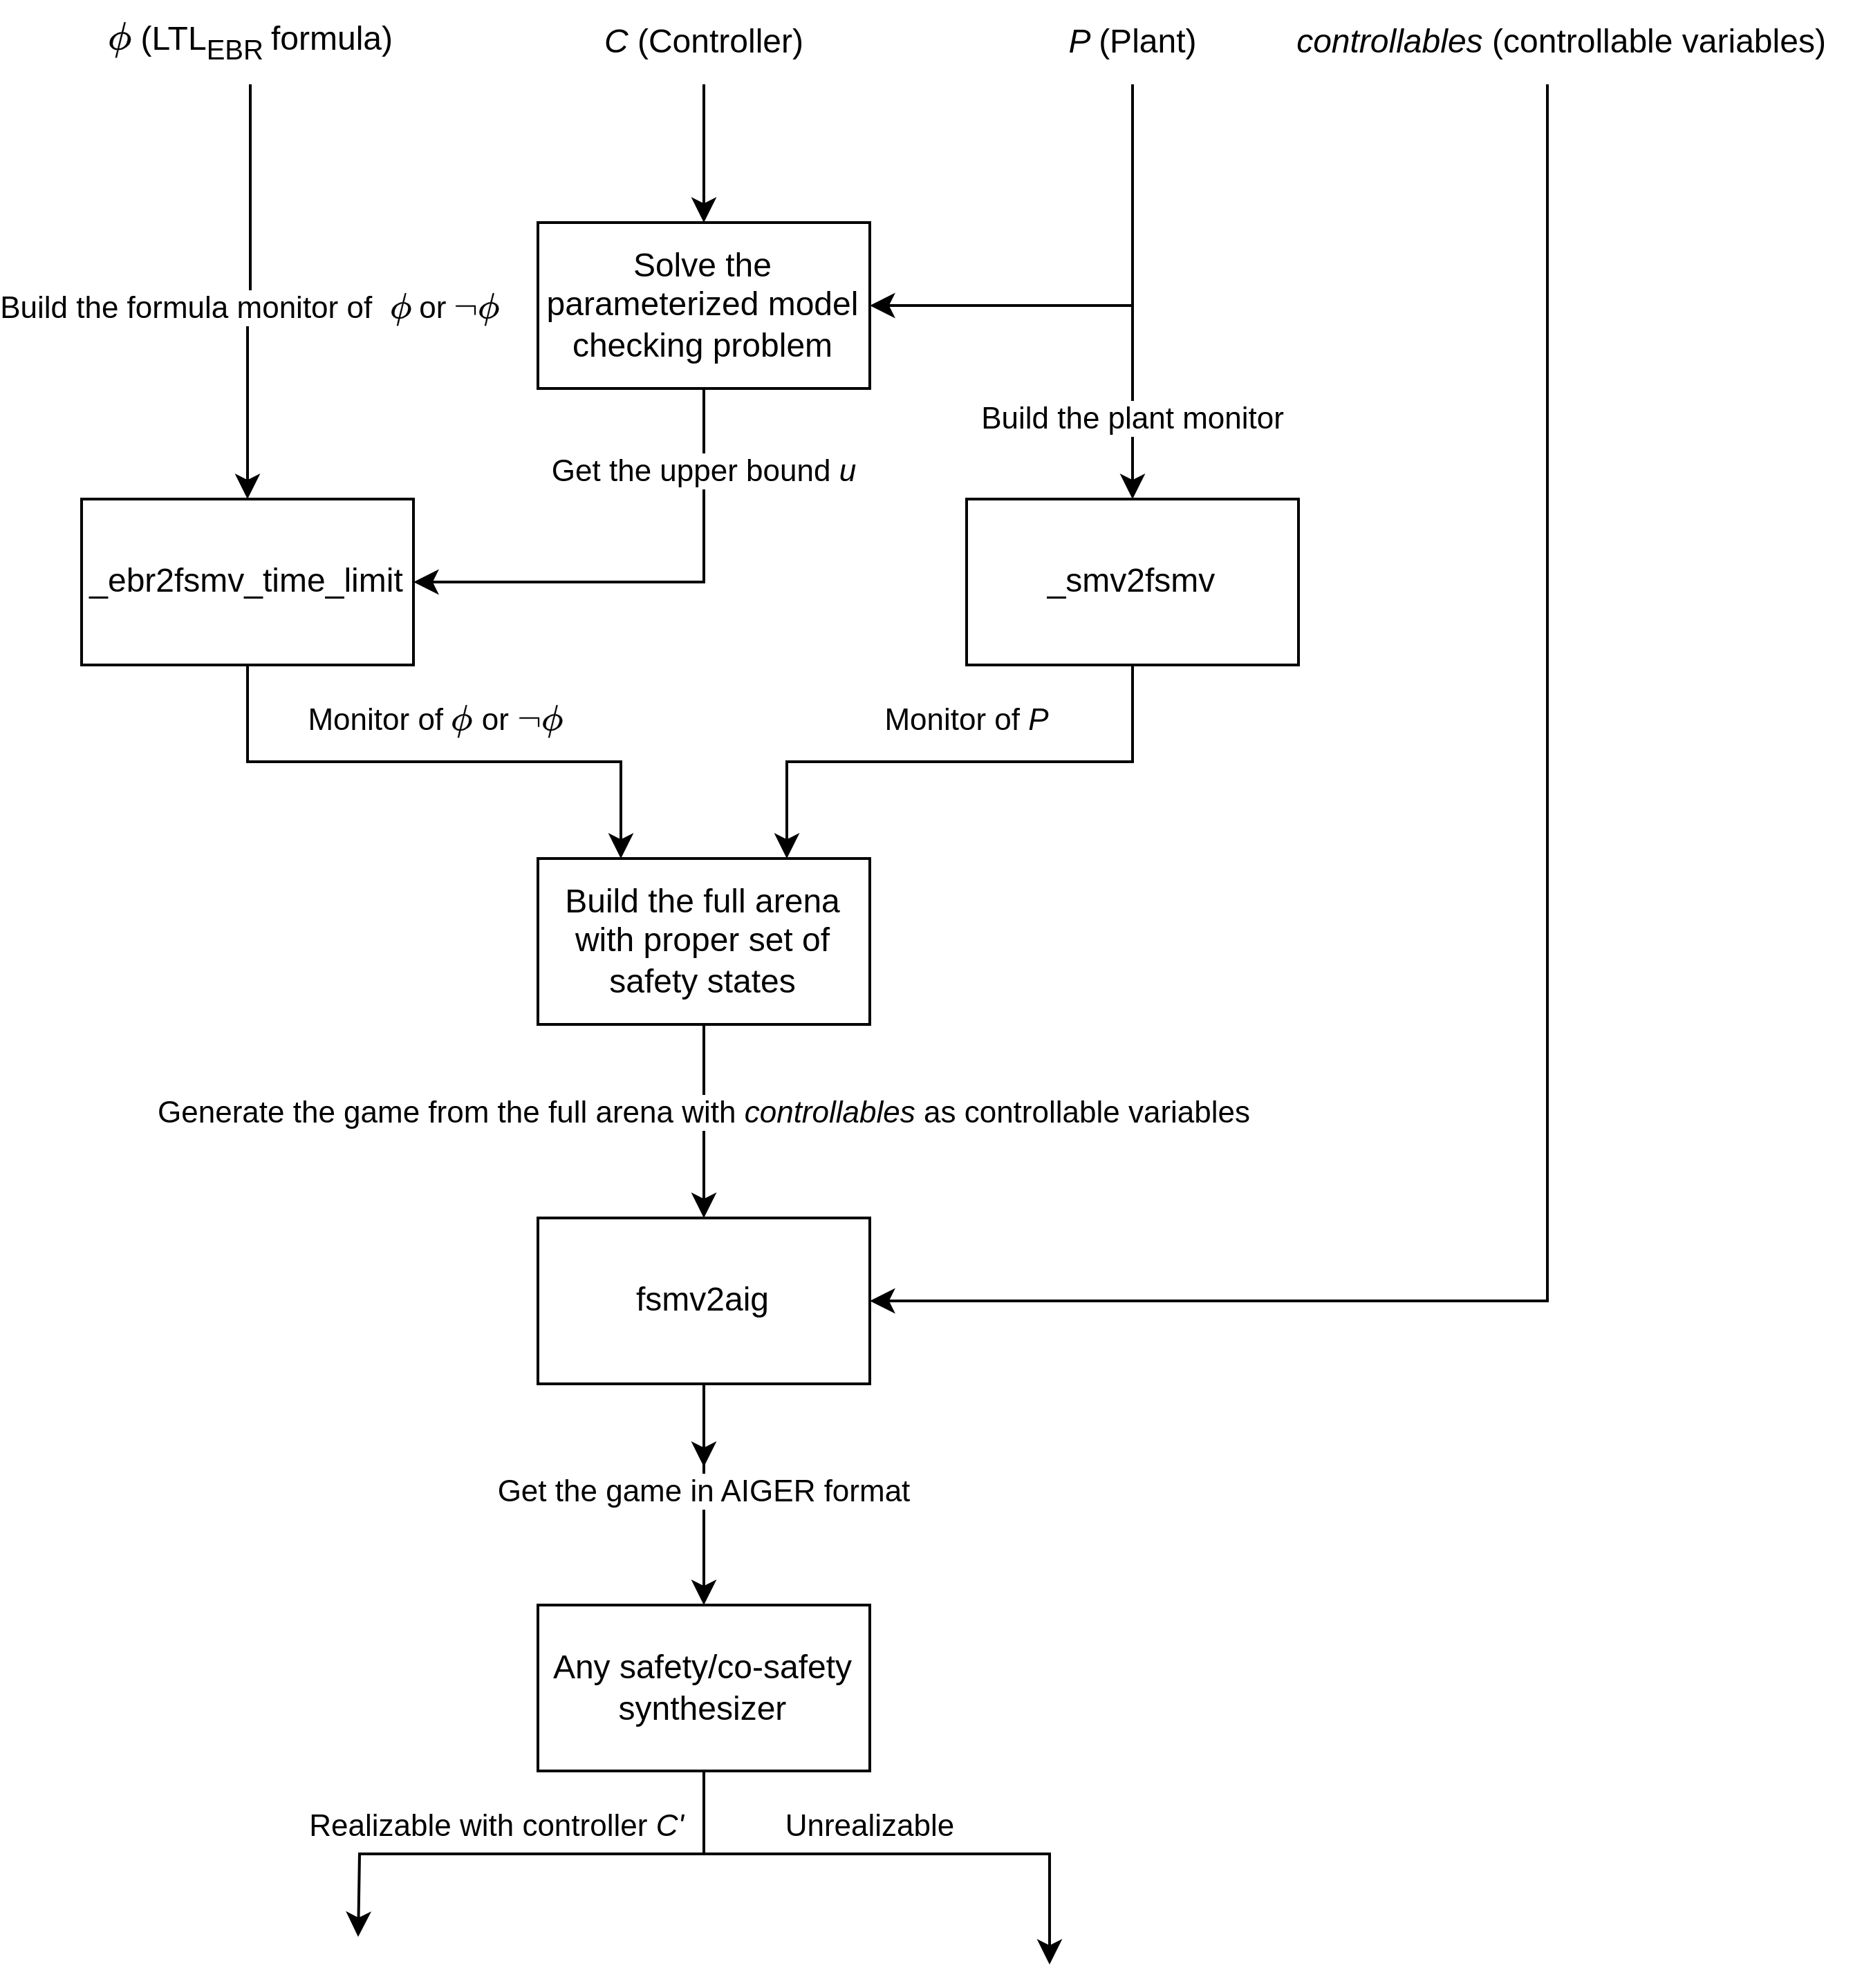
\includegraphics[width=0.6\linewidth]{figures/optimality-algorithm-asap.png}
    \caption{The optimality test algorithm for ASAP semantics graphically}
    \label{fig:asap-optimality}
\end{figure}

\section{Notable example}
In this section we show a notable example of the previous algorithm. It is useful to fix all concepts we have seen so far. As notable example we have chosen the ferryman puzzle which has already been introduced in \autoref{sec:smv} and for this reason we will not explain it again. 
Our aim is to satisfy the formula $\phi$ ASAP.
\begin{flalign*}
\ltlU{(\ltlImpl{(\ltlOr{\text{goat=wolf}}{\text{goat=cabbage}})}{\text{goat=man}})}{(\text{goat} \land \text{cabbage} \land \text{wolf} \land \text{man})}
\end{flalign*}

However, we need to make some changes to make it suitable for the optimality test algorithm.
First of all, we need to convert the plant to functional SMV format. 
The original plant is described through \lstinline{init} and \lstinline{next} statements, but it contains some atomic values and our tools cannot cope with them.
Therefore, we encode \lstinline{move} through two boolean variables, i.e. \lstinline{move0} and \lstinline{move1}, and each combination of them defines a move.

\begin{lstlisting}[language=smv, caption=Ferryman ASAP: plant in functional SMV format]
MODULE plant(move0,move1)
VAR
    man     : boolean;
    wolf    : boolean;
    goat    : boolean;
    cabbage : boolean;
DEFINE
    no_carry      := !move0 & !move1; -- move=e
    carry_goat    := move0  & !move1; -- move=g
    carry_wolf    := !move0 & move1;  -- move=w
    carry_cabbage := move0  & move1;  -- move=c
ASSIGN
    init(man)     := FALSE;
    init(goat)    := FALSE;
    init(wolf)    := FALSE;
    init(cabbage) := FALSE;
ASSIGN
next(cabbage) := case
  (carry_cabbage & (cabbage=man)) : !cabbage;
  TRUE : cabbage;
esac;
next(goat) := case
  (carry_goat & (goat=man)) : !goat;
  TRUE : goat;
esac;
next(wolf) := case
  (carry_wolf & (wolf=man)) : !wolf;
  TRUE : wolf;
esac;
next(man) := !man;
DEFINE
    safe_state := (goat=wolf | goat=cabbage) -> goat=man;
    goal := cabbage & goat & wolf & man;
\end{lstlisting}

After having defined the plant, let us define the controller.
For demonstration purposes we define a controller which is slower than the optimal one of two steps, introducing a delay at the beginning forcing an unnecessary carrying of the goat.

\begin{lstlisting}[language=smv, caption=Ferryman ASAP: slow controller]
MODULE SlowController(man, goat, wolf, cabbage)
VAR
-- possible moves
  move0 : boolean;
  move1 : boolean;
  delay : boolean;
INIT
  delay
TRANS
  next(delay) <-> (delay & !man)
ASSIGN
  move0 :=
    case
      !man:
        case
          man=cabbage & man=goat & man=wolf: TRUE;
          man=cabbage & man=goat: TRUE;
          man=cabbage & man=wolf: FALSE;
          man=cabbage: TRUE;
          man=goat & man=wolf: FALSE;
          man=goat : TRUE;
          man=wolf : FALSE;
          TRUE : FALSE;
        esac;
      TRUE:
        case
          delay : TRUE;
          man=cabbage & man=goat: TRUE;
          man=goat & man=wolf: TRUE;
          TRUE: FALSE;
        esac;
    esac;
ASSIGN
  move1 :=
    case
      !man:
        case
          man=cabbage & man=goat & man=wolf: FALSE;
          man=cabbage & man=goat: TRUE;
          man=cabbage & man=wolf: TRUE;
          man=cabbage: TRUE;
          man=goat & man=wolf: TRUE;
          man=goat : FALSE;
          man=wolf : TRUE;
          TRUE : FALSE;
        esac;
      TRUE:
        case
          delay : FALSE;
          man=cabbage & man=goat: TRUE;
          man=goat & man=wolf: FALSE;
          TRUE: FALSE;
        esac;
    esac;
\end{lstlisting}

We can now compute the upper-bound $u$ required by the algorithm to find out whether there exists a controller which enforces the formula in a smaller number of steps.
To discover this bound we need to solve a parameterized model checking problem on the maximum number of steps that can be performed enforcing the formula and look for the minimum value among those values.
In SMV a parameterized model checking problem is formulated in the following way:
\begin{lstlisting}[language=smv, caption=Ferryman ASAP: parameterized model checking problem with until operator]
MODULE main
VAR
  p: Plant(c.move);
  c: SlowController(p.cabbage, p.goat, p.wolf, p.man);
-- Parameterized model checking problem
VAR time: 0..10;
FROZENVAR maxtime: 0..10;
ASSIGN
  init(time) := 0;
  next(time) := case time < 10 : time + 1; TRUE: time; esac;
  PARSYNTH r := { maxtime | VALID (p.safe_state U (p.goal & time<=maxtime)) };
\end{lstlisting}

Basically, we introduce two variables: \lstinline{time} and \lstinline{maxtime}.
The first one counts the number of steps already performed, while the second one is the parameter to synthesize. So we look for the fixed values of \lstinline{maxtime} for which the formula is satisfied.
It is easy to see that when \lstinline{maxtime} is too low we cannot satisfy the right side of until temporal operator and so the whole formula is false.
For efficiency reasons we convert this formula to an equivalent safety formula. That is because, as we have already seen, is possible to reduce the model checking of safety formulas to an invariant verification problem, which is more efficient.
We rewrite the formula in terms of release (in NuSMV the release symbol is \lstinline{V}), where whenever we exceed the time we need to satisfy the goal as well, otherwise the whole formula will be false.

\begin{lstlisting}[language=smv, caption=Ferryman ASAP: parameterized model checking problem with release operator]
PARSYNTH r := { maxtime | VALID (p.goal V (p.safe_state & time<=maxtime)) };
\end{lstlisting}

By executing the following commands to solve the parameterized model checking problem in the nuXmv CLI, we can see that the least upper-bound to \lstinline{maxtime} is $9$.
Therefore we can state that \lstinline{Plant} is satisfied ASAP by \lstinline{ControllerSlow} in $9$ steps.
\begin{lstlisting}[language=bash, caption=Ferryman ASAP: commands to execute to solve the parameterized model checking problem]
nuXmv > go_bmc
nuXmv > synth_param -a ic3 -s -l -c
nuXmv > show_param_synth_problems  
There is 1 param synth problem:
001: SYNTH r := { maxtime | VALID !(!p.goal U !(p.safe_state & time <= maxtime)) }, region: (maxtime = 10 | maxtime = 9)
\end{lstlisting}

Now we look for a controller which can satisfy the formula in less steps.
First of all we generate the plant monitor by \lstinline{_smv2fsmv} tool. 

\begin{lstlisting}[language=smv, caption=Ferryman ASAP: plant monitor]
MODULE monitor_0(move0,move1,man,wolf,goat,cabbage)
VAR
   MON_0_ERROR_cabbage : boolean;
   MON_0_SIM_cabbage : boolean;
   MON_0_ERROR_goat : boolean;
   MON_0_SIM_goat : boolean;
   MON_0_ERROR_wolf : boolean;
   MON_0_SIM_wolf : boolean;
   MON_0_ERROR_man : boolean;
   MON_0_SIM_man : boolean;
DEFINE
   MON_0_ERROR := (MON_0_ERROR_wolf | (MON_0_ERROR_man | (MON_0_ERROR_cabbage | MON_0_ERROR_goat)));
   no_carry := (!move0 & !move1);
   carry_goat := (move0 & !move1);
   carry_wolf := (!move0 & move1);
   carry_cabbage := (move0 & move1);
ASSIGN
   init(MON_0_ERROR_wolf) := FALSE;
   init(MON_0_SIM_wolf) := FALSE;
   init(MON_0_ERROR_man) := FALSE;
   init(MON_0_SIM_man) := FALSE;
   init(MON_0_ERROR_cabbage) := FALSE;
   init(MON_0_SIM_cabbage) := FALSE;
   init(MON_0_ERROR_goat) := FALSE;
   init(MON_0_SIM_goat) := FALSE;
ASSIGN
   next(MON_0_SIM_wolf) := case
    (carry_wolf & (MON_0_SIM_wolf<->MON_0_SIM_man)) : !MON_0_SIM_wolf;
    TRUE : MON_0_SIM_wolf;
   esac;
   next(MON_0_SIM_cabbage) := case
    (carry_cabbage & (MON_0_SIM_cabbage <-> MON_0_SIM_man)) : !MON_0_SIM_cabbage;
    TRUE : MON_0_SIM_cabbage;
   esac;
   next(MON_0_SIM_goat) := case
    (carry_goat & (MON_0_SIM_goat <-> MON_0_SIM_man)) : !MON_0_SIM_goat;
    TRUE : MON_0_SIM_goat;
   esac;
   next(MON_0_SIM_man) := !MON_0_SIM_man;
ASSIGN
   next(MON_0_ERROR_man) := (MON_0_ERROR_man | (MON_0_SIM_man != man));
   next(MON_0_ERROR_wolf) := (MON_0_ERROR_wolf | (MON_0_SIM_wolf != wolf));
   next(MON_0_ERROR_cabbage) := (MON_0_ERROR_cabbage | (MON_0_SIM_cabbage != cabbage));
   next(MON_0_ERROR_goat) := (MON_0_ERROR_goat | (MON_0_SIM_goat != goat));
\end{lstlisting}

Then, since $\phi$ is a co-safety formula, we negate it and generate the monitor of the negated formula by \lstinline{_ebr2fsmv_time_limit} tool with bound $8$.

\begin{lstlisting}[language=smv, caption=Ferryman ASAP: formula monitor with bound $8$]
MODULE ltl_spec_0(move0,move1,man,wolf,goat,cabbage)
VAR
   EBR_0_PAST_1 : boolean;
   EBR_0_ERROR_0 : boolean;
   EBR_0_COUNTER_4 : boolean;
   EBR_0_COUNTER_3 : boolean;
   EBR_0_COUNTER_2 : boolean;
   EBR_0_COUNTER_1 : boolean;
   EBR_0_COUNTER_0 : boolean;
DEFINE
   EBR_0_ERROR := (!EBR_0_EXPIRED & EBR_0_ERROR_0);
   EBR_0_EXPIRED := !(!EBR_0_COUNTER_4 & (!EBR_0_COUNTER_3 | (!EBR_0_COUNTER_2 & !EBR_0_COUNTER_1)));
ASSIGN
   init(EBR_0_PAST_1) := FALSE;
   init(EBR_0_ERROR_0) := FALSE;
   init(EBR_0_COUNTER_4) := FALSE;
   init(EBR_0_COUNTER_3) := FALSE;
   init(EBR_0_COUNTER_2) := FALSE;
   init(EBR_0_COUNTER_1) := FALSE;
   init(EBR_0_COUNTER_0) := FALSE;
ASSIGN
   next(EBR_0_PAST_1) := case
    ((((!goat | wolf) & (!wolf | goat)) | ((!goat | cabbage) & (!cabbage | goat))) & ((goat & !man) | (man & !goat))) : TRUE;
    EBR_0_PAST_1 : TRUE;
   TRUE : FALSE;
esac;
ASSIGN
   next(EBR_0_ERROR_0) := case
    (!EBR_0_ERROR_0 & EBR_0_PAST_1) : FALSE;
    (!EBR_0_ERROR_0 & (((((!goat | wolf) & (!wolf | goat)) | ((!goat | cabbage) & (!cabbage | goat))) & ((goat & !man) | (man & !goat))) & (((!cabbage | !goat) | !wolf) | !man))) : FALSE;
    (!EBR_0_ERROR_0 & (((!cabbage | !goat) | !wolf) | !man)) : FALSE;
    TRUE : TRUE;
   esac;
ASSIGN
   next(EBR_0_COUNTER_4) := (((((EBR_0_COUNTER_0 & EBR_0_COUNTER_1) & EBR_0_COUNTER_2) & EBR_0_COUNTER_3) & EBR_0_COUNTER_4) | ((EBR_0_COUNTER_3 & (EBR_0_COUNTER_2 & (EBR_0_COUNTER_1 & EBR_0_COUNTER_0))) <-> !EBR_0_COUNTER_4));
ASSIGN
   next(EBR_0_COUNTER_3) := (((((EBR_0_COUNTER_0 & EBR_0_COUNTER_1) & EBR_0_COUNTER_2) & EBR_0_COUNTER_3) & EBR_0_COUNTER_4) | ((EBR_0_COUNTER_2 & (EBR_0_COUNTER_1 & EBR_0_COUNTER_0)) <-> !EBR_0_COUNTER_3));
ASSIGN
   next(EBR_0_COUNTER_2) := (((((EBR_0_COUNTER_0 & EBR_0_COUNTER_1) & EBR_0_COUNTER_2) & EBR_0_COUNTER_3) & EBR_0_COUNTER_4) | ((EBR_0_COUNTER_1 & EBR_0_COUNTER_0) <-> !EBR_0_COUNTER_2));
ASSIGN
   next(EBR_0_COUNTER_1) := (((((EBR_0_COUNTER_0 & EBR_0_COUNTER_1) & EBR_0_COUNTER_2) & EBR_0_COUNTER_3) & EBR_0_COUNTER_4) | (EBR_0_COUNTER_0 <-> !EBR_0_COUNTER_1));
ASSIGN
   next(EBR_0_COUNTER_0) := (((((EBR_0_COUNTER_0 & EBR_0_COUNTER_1) & EBR_0_COUNTER_2) & EBR_0_COUNTER_3) & EBR_0_COUNTER_4) | !EBR_0_COUNTER_0);
\end{lstlisting}

At this point we have all required monitors with the corresponding errors variables, i.e. \lstinline{EBR_0_ERROR} for the monitor of the negated formula and \lstinline{MON_0_ERROR} for the monitor of the plant.
We make synchronous product between the two monitors and set the correct \lstinline{INVARSPEC}.
Note that, contrary to how we defined this part in \autoref{sec:reduction-to-synthesis}, we do not need the additional variable \lstinline{in_bound} because we force the bound directly in the formula monitor with \lstinline{EBR_0_EXPIRED}.

\begin{lstlisting}[language=smv, caption=Ferryman ASAP: main module]
MODULE main
IVAR
    man : boolean;
    goat : boolean;
    wolf : boolean;
    cabbage : boolean;
    move0 : boolean;
    move1 : boolean;
VAR
   m : monitor_0(move0,move1,man,wolf,goat,cabbage);
   p : ltl_spec_0(move0,move1,man,wolf,goat,cabbage);
INVARSPEC !m.MON_0_ERROR & !p.EBR_0_ERROR
\end{lstlisting}

Finally we have the whole arena which can be converted to AIGER format by \lstinline{fsmv2aig} tool where we specify the controllable variables, i.e. \lstinline{move0} and \lstinline{move1}.
We end up with the game in AIGER format which can be solved by any synthesizer.
The output of the execution of \lstinline{simplesynth} synthesizer on the game is that the game is realizable and it provides us a new controller which is better than the given one.
Indeed, if we solve the parameterized model checking on the closed-loop of the plant with the new controller, we see that the formula is satisfied in $7$ steps instead of the previous $9$ steps.
Moreover, if we repeat the whole algorithm with the new controller, we note that there is no other controller better than the current one and therefore we state that the synthesized controller is also optimal.

%!TEX root = ../main.tex
\chapter{Conclusion and Future Work} \label{chapt:conclusion}
% Conclusione e lavori futuri.

In this thesis we have studied the problem of testing the optimality of a controller under a specific optimality principle.
More formally, the problem we have faced is: given a plant, a controller and a safety or co-safety $\ltl$ formula satisfied in the closed-loop between plant and controller, we want to figure out whether such controller is the best one satisfying that formula for the plant according to an optimality principle.

To define the concept of optimal controller we need to define two semantics: bounded-value semantics and best-effort semantics.
The first semantics is useful to add a further constraint to a variable and forcing it to be lower than a bound $u$ given a-priori.
The best-effort semantics is defined exploiting the bounded-value semantics as follows: a formula is satisfied best-effort by a state-sequence with bound $u^*$ if and only if $u^*$ is the least upper bound to the bounds making that formula satisfied bounded-value by that state-sequence.
In other words, if we take any $u' \prec u^*$ as new bound, it must hold that formula is not satisfied by the state-sequence.

Moreover, we have presented other two semantics: bounded-steps semantics and As Soon As Possible (ASAP) semantics.
The first semantic forces a formula to be satisfied in a bounded number of steps, while the latter one forces a formula to be satisfied in the smallest number of steps.
As for the previous two semantics, ASAP semantics is defined exploiting bounded-steps semantics as follows: a formula is satisfied ASAP by a state-sequence in $u$ steps, if it is satisfied bounded-steps in $u$ steps but not satisfied in $u-1$ steps.
Later we have proved the correspondence between ASAP and best-effort semantics, pointing out the fact that bounded-steps and ASAP semantics are just one of the possible instances of bounded-value and best-effort semantics.  

In our case we have considered the best-effort semantics to define the optimality principle, since it is the most general one. 
Therefore, a controller is said optimal if and only if it satisfies a formula with bound $u^*$ under best-effort semantics and there does not exist any other controller satisfying the same formula with any lower bound, i.e. any $u' \prec u^*$.

Afterwards, we have proposed a way to solve the optimality check by reduction to a reactive synthesis problem. In particular, we figure out whether the given controller is optimal or not, by reducing the synthesis of a new controller with a lower bound to solving a safety or a reachability game, depending on the type of property we want to synthesize. If the property is a safety property, then we play a safety game, while if the property is a co-safety property, then we play a reachability game.
The arena on which we play the game is always a safety arena and we exploit the duality between safety and reachability games to synthesize correctly the formula with the plant as assumptions. The arena on which we play the game is a constrained arena obtained from the synchronous product between formula arena and plant arena (the assumptions), to which we add additional constraints to force the synthesis of a better controller. If the game is not realizable, then it means that the given controller is optimal and we cannot do better than that, while if the game is realizable, it means that there exists a better controller which corresponds to the one just synthesized. 

The optimality test described above has been implemented in nuXmv and, to solve the game, it exploits a safety and reachability synthesizer made from scratch by us.

In conclusion, let us see some possible future works on this topic.
One possible future work is to generalize the optimality principle with a generic cost function instead of the "less than u" bound.
Consequently, the meaning of best-effort semantics would change and would allow to express scenarios where the cost of enforcing a property depends not only on the number of steps, but also on the specific action taken by the controller, or by some other factors such as the energy consumption or the resources needed to take an action.
A further possible future work is to implement an iterative algorithm to get the optimal controller starting from a non optimal one in the ASAP semantics.
Such iterative algorithm behaves as follows: starting from an initial controller, if a better controller is not realizable, then it means that such controller is optimal, otherwise repeat the cycle with the improved controller returned by the optimality test.
Since we lower the bound at each iteration, and the bound is a non-negative integer, such algorithm does not diverge and it is ensured to not reach sub-optimal controllers.
Finally, it would be interesting to apply the concept of optimal controller given by best-effort semantics to distributed systems, reducing the problem to a distributed reactive synthesis problem.


\cleardoublepage
\nocite{*}
\phantomsection
\addcontentsline{toc}{chapter}{References}
\bibliography{references}

\cleardoublepage
\phantomsection
\addcontentsline{toc}{chapter}{Acknowledgments}
\acknowledgments

\end{document}
